\documentclass{article}

\title{Income and Consumption Inequality in Taiwan, 1981 - 2023}
\author{Bo-Yan Huang\footnote{Department of Economics, National Taiwan University, Taipei, Taiwan}}
\date{June 2025}

% Bring in setting.tex
\usepackage[a4paper,top=2cm,bottom=2cm,left=3cm,right=3cm,marginparwidth=1.75cm]{geometry}
\usepackage{graphicx}
\usepackage[colorlinks=true, allcolors=blue]{hyperref}
\usepackage{setspace}
\usepackage{subcaption}
\usepackage{mwe}

\setstretch{1.3}
\setlength\parindent{2em}

\begin{document}
\maketitle

\section{Introduction}
\label{sec:introduction}

In Taiwan, the evolution of economic inequality is often overshadowed by other topics in the field of economics.
However, understanding the dynamics of inequality is crucial for comprehending the broader economic landscape. 
Most studies on inequality in Taiwan have focused on income distribution and income gap, with less attention given to consumption inequality.
For instance, Chang, Lin, and Lee (2022) analyzed the income distribution in Taiwan from 1990 to 2020, highlighting the increase in income and education inequality during this period.
The authors apply the Age-Period-Cohort (APC) model to reveal that classes and education inequality primarily drive the increase in income inequality, and the generational gap between the baby boomers and millennials does not decrease over time. 
At the same time, Chang (2023) focused on the impact of government redistribution and political parties' actions. 
The author points out that the Democratic Progressive Party (DPP) share in the Legislative Yuan is negatively correlated with income inequality. However, a president from the DPP is negatively correlated with redistribution, which could worsen income inequality in the long run.
Both studies use the Survey of Family Income and Expenditure (SFIE) as their primary data set. This repeated cross-sectional survey, started in 1978 and conducted yearly, provides detailed information on Taiwan's household income and expenditure patterns.

Consumption inequality has been less frequently studied in Taiwan. Hong (2012) used the SFIE from 1980 to 2007 to analyze the evolution of consumption inequality in Taiwan, focusing on the Gini coefficient and the dynamics of consumption percentiles. 
The study found that consumption inequality decreased after 1996 due to the redistribution effect of public health insurance in Taiwan and the growing elderly population in our demographic structure.
However, the decrease in consumption inequality could be a double-edged sword since the other reason for the decline is the low consumption growth rate of wealthy families, which could lead to an economy that stagnates.

One reason for the lack of attention to consumption in Taiwan and other countries is the difficulty in measuring consumption accurately.
First, unlike income, which can be directly observed through tax records, consumption is often inferred from expenditure data that the government does not document.
Therefore, most consumption data are often collected through surveys, which have a smaller sample size and are more prone to measurement errors and biases.
Currently, the SFIE is the only survey that provides detailed information on household consumption in Taiwan, while The Consumer Expenditure Survey (CE) is the only one in the US (Attanasio \& Pistaferri, 2016).

Second, the transformation from expenditure to consumption is not straightforward. Surveys like the SFIE typically report household expenditures, which may not accurately reflect households' actual consumption.
For example, households may purchase goods in bulk or invest in durable goods, which can lead to discrepancies between expenditure and consumption. Most surveys lack information on the stock of durable goods and their current value.
Another example is that consumption can be produced at home using time and goods, like childcare and home-cooked meals. Also, households may have different preferences for leisure and consumption, which can lead to differences in how they allocate their resources.
The most difficult problem to overcome is the assumption that all households face the same prices for goods and services. This assumption violates the nature of durable goods such as housing and automobiles, which can have enormous price variations. Ignoring these differences can lead to an inaccurate representation of consumption patterns and inequality.

This paper uses SFID data to comprehensively analyze income and consumption inequality in Taiwan from 1981 to 2023 to fill in the missing pieces of inequality dynamics after 2008. This is interesting because economic growth in Taiwan has slowed since the 2008 financial crisis, and the COVID-19 pandemic has further exacerbated the situation.
The income distribution between households was stable before 1994, and the Gini coefficient for individual earnings stabilized at around 0.30 due to many factors (Bourguignon, Fournier, \& Gurgand, 2001).
However, the Gini coefficient for household earnings has increased since 1994, reaching 0.35 in 2023, as shown in the top right panel of Figure \ref{fig:Indi_to_HH}.
This suggests that economic inequality will become a problem after economic growth slows down, even in a country with steady income distribution previously, like Taiwan.
The paper is organized as follows: Section \ref{sec:data} describes the data used in the analysis, Section \ref{sec:household_inequality} presents the household-level inequality measures, including earnings, consumption, and their cyclical dynamics, and Section \ref{sec:conclusion} concludes the paper.


\section{Data}
\label{sec:data}

\subsection{Survey of Family Income and Expenditure (SFIE)}
The data used in this paper is the SFIE, which is a repeated cross-sectional survey conducted annually since 1978 by the Directorate-General of Budget, Accounting and Statistics (DGBAS) in Taiwan.
The survey provides a rich dataset for analyzing income and expenditure patterns, including earnings, private transfers, asset income, government transfers, and consumption expenditures.
The survey samples around 16,000 households each year, however the response rate of certain columns, such as labor earnings and  

\subsection{Equivalizing}


\section{Household-level Inequality}
\label{sec:household_inequality}

\subsection{Inequality in Earnings}

\begin{figure}
    \centering
    \begin{subfigure}[t]{0.475\textwidth}
        \centering
        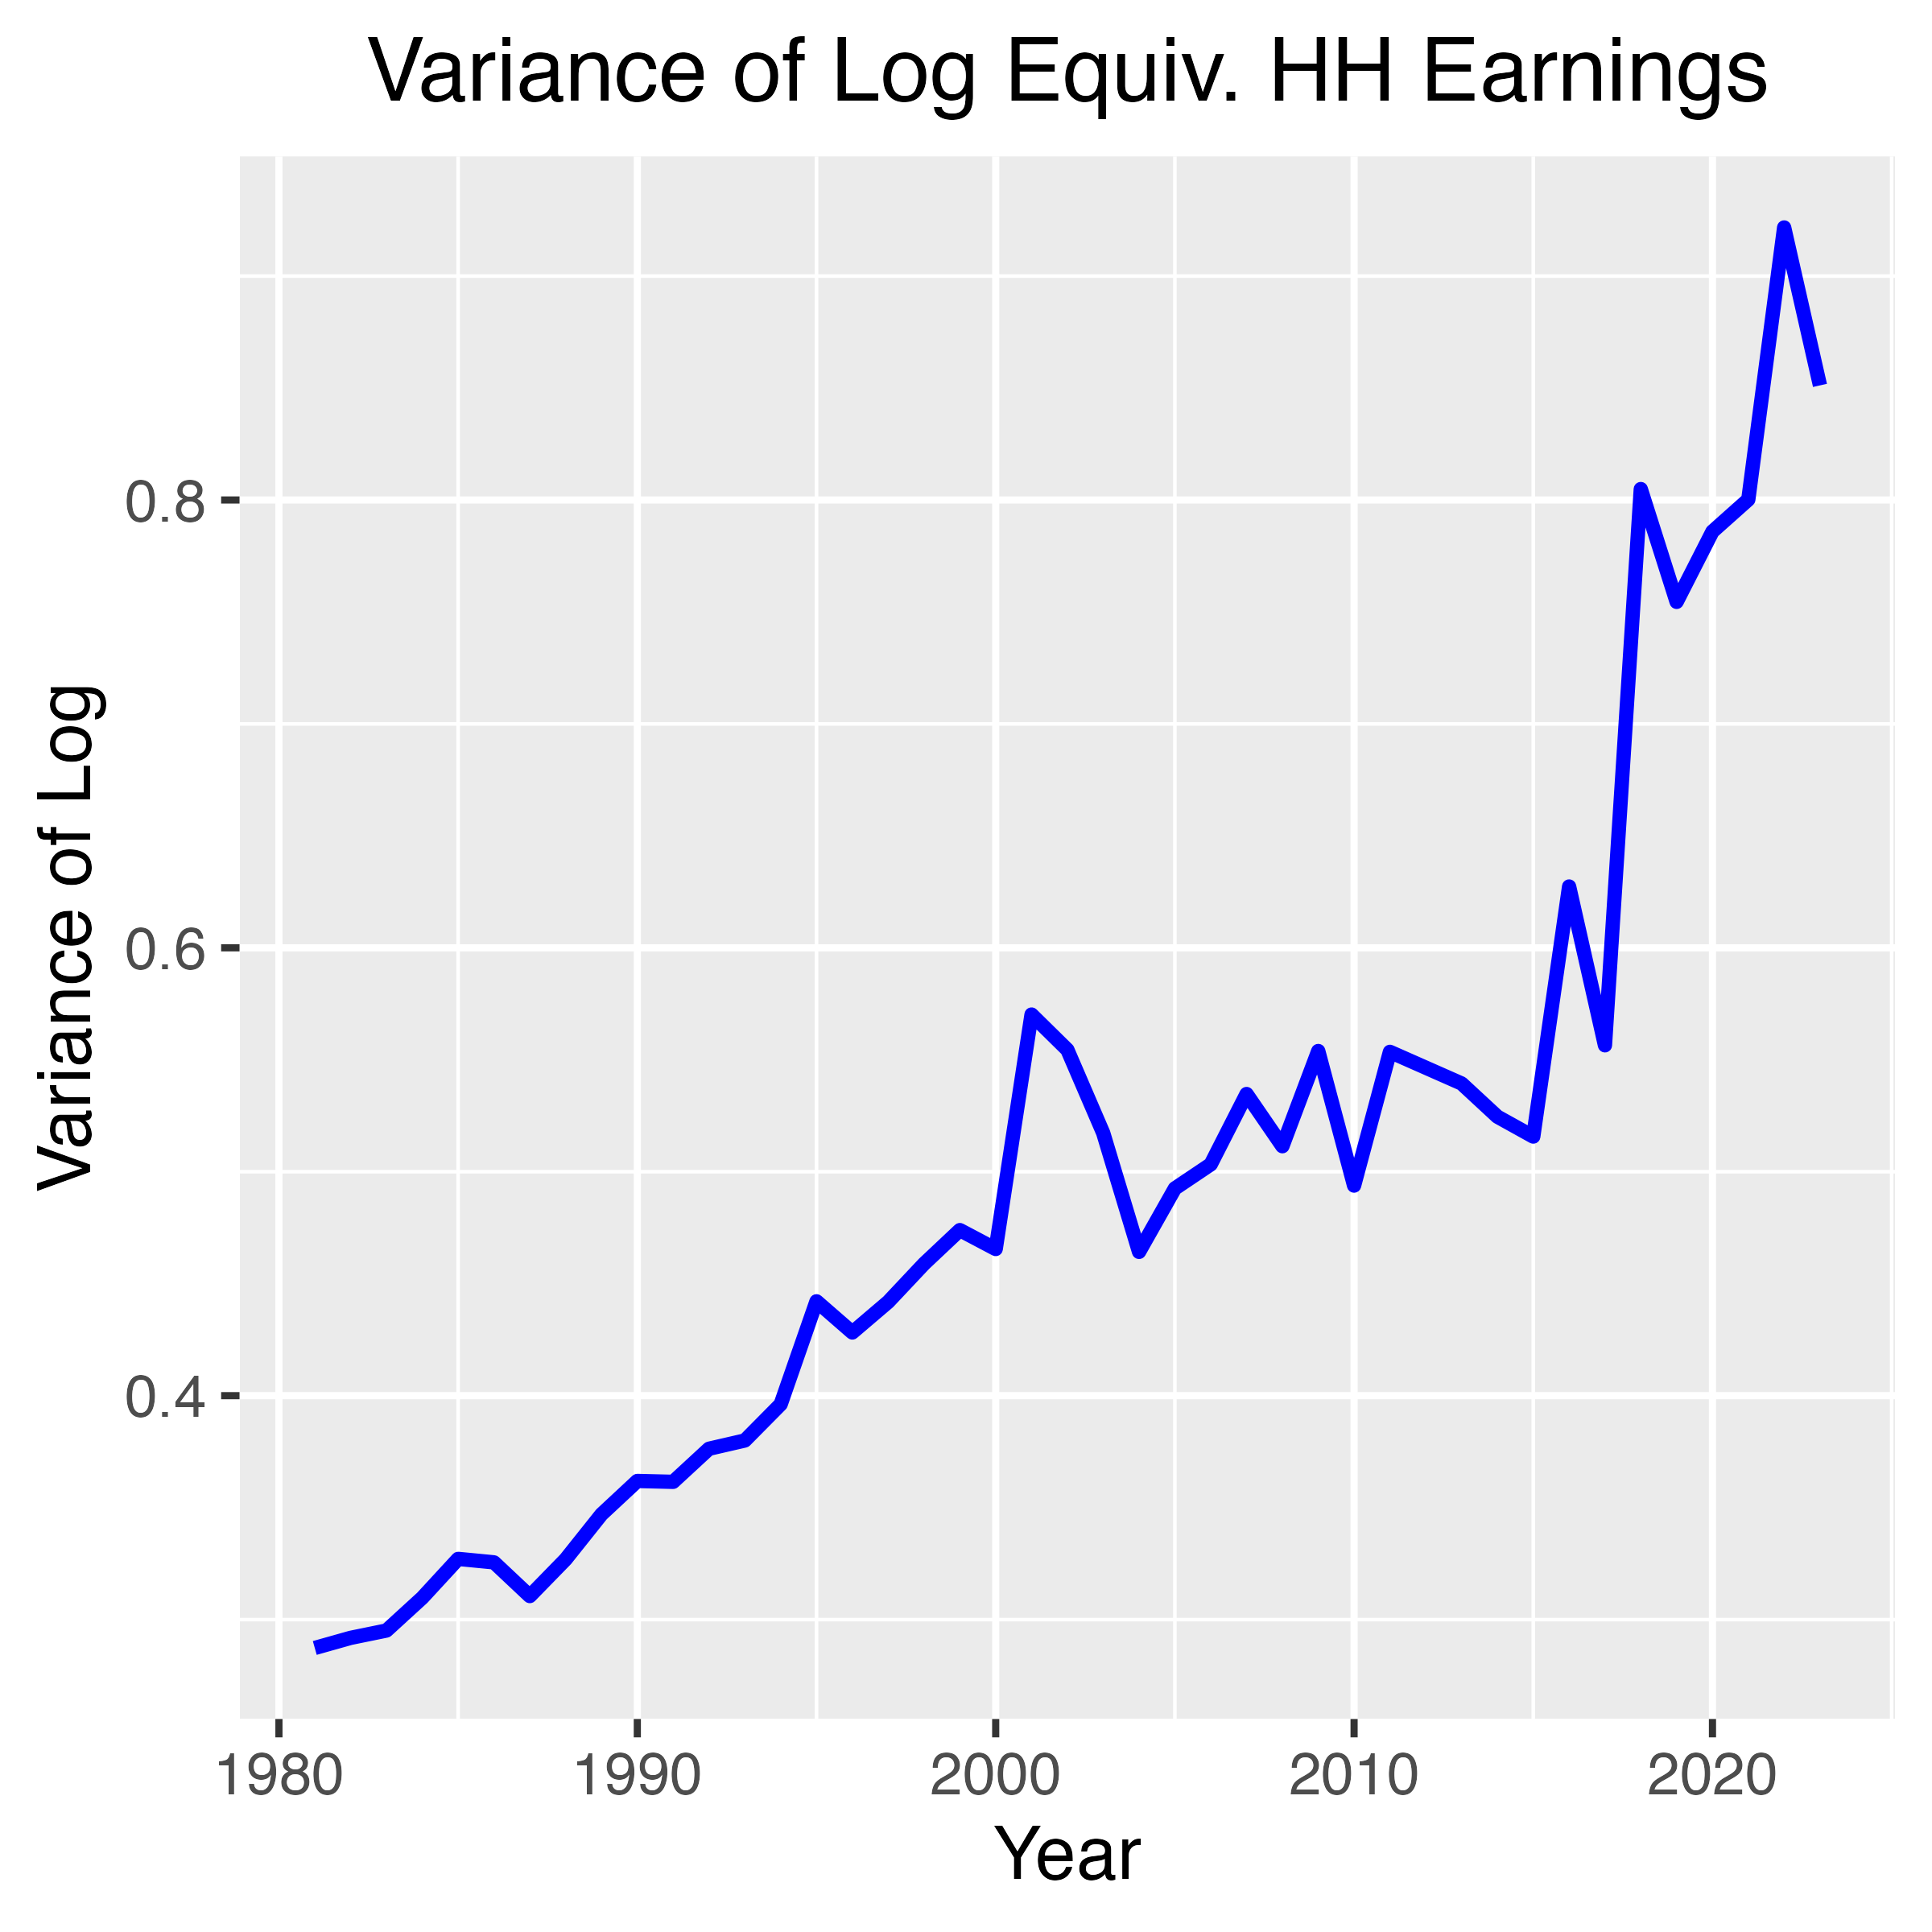
\includegraphics[width=\textwidth]{figures/Fig_1/Fig_1a_Var_Earnings.png}
        \label{fig:earnings_inequality_Var}
    \end{subfigure}
    \begin{subfigure}[t]{0.475\textwidth}
        \centering
        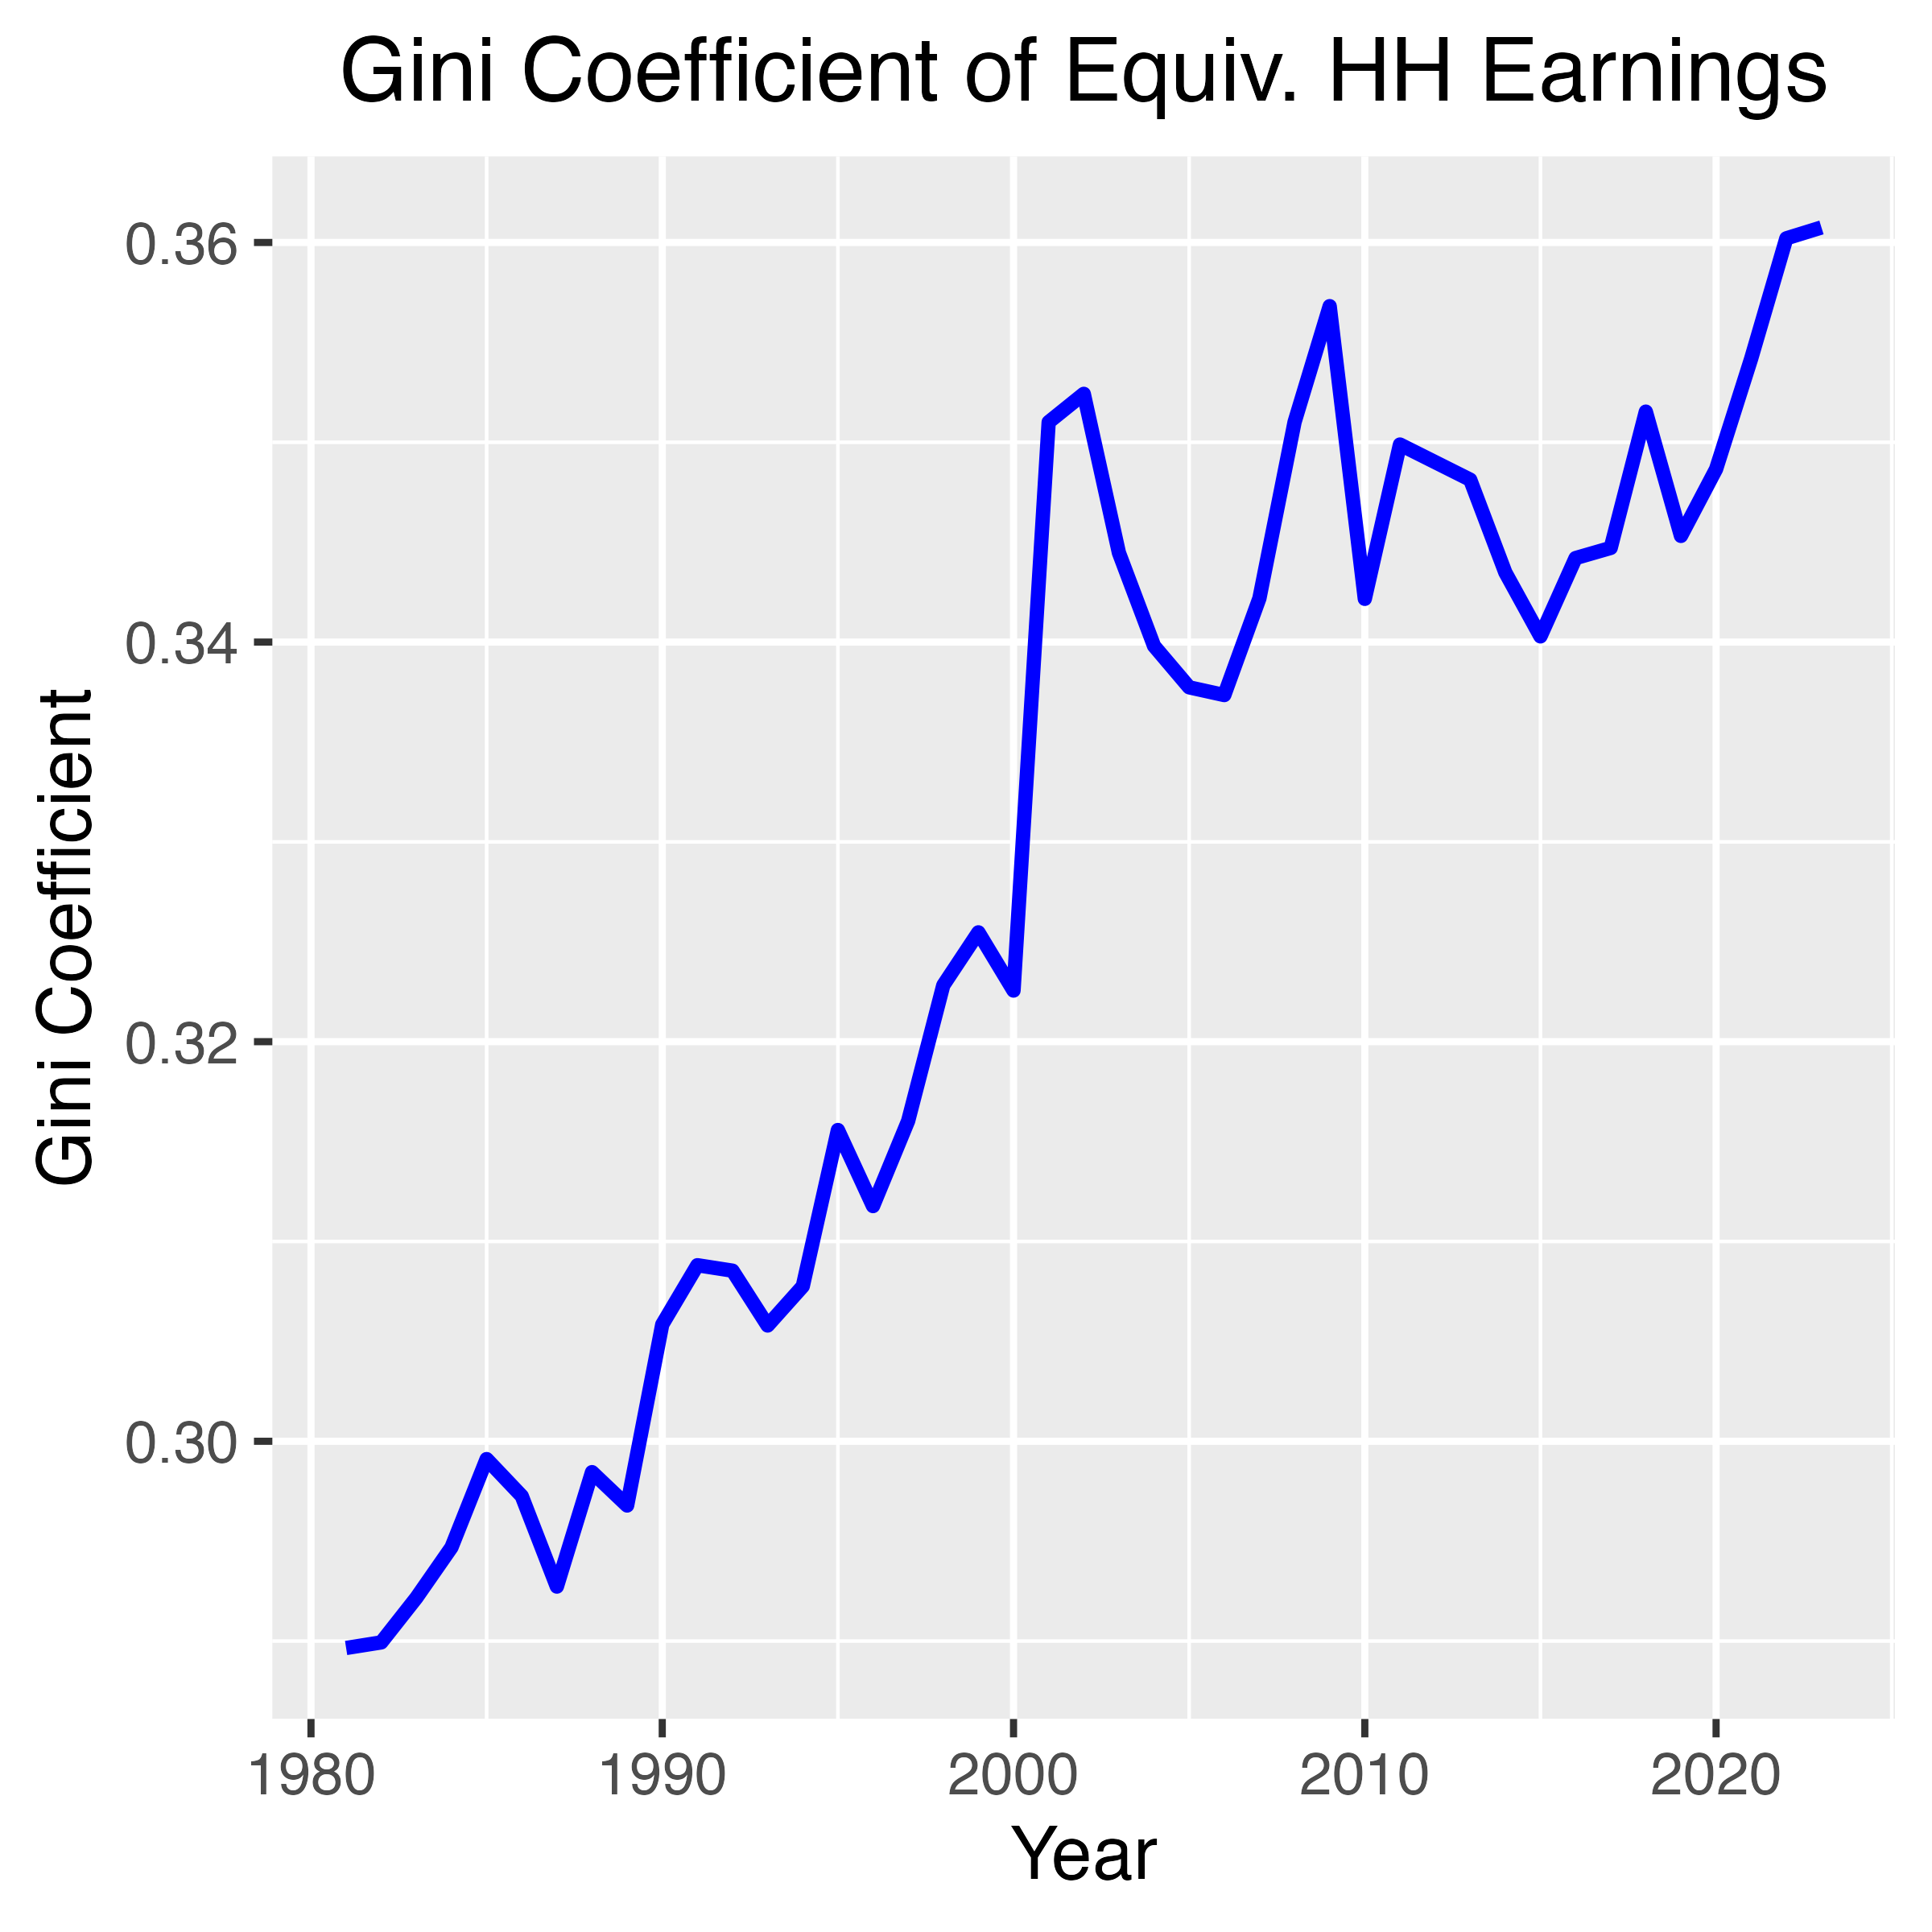
\includegraphics[width=\textwidth]{figures/Fig_1/Fig_1b_Gini_Earnings.png}
        \label{fig:earnings_inequality_Gini}
    \end{subfigure}
    \begin{subfigure}[t]{0.475\textwidth}
        \centering
        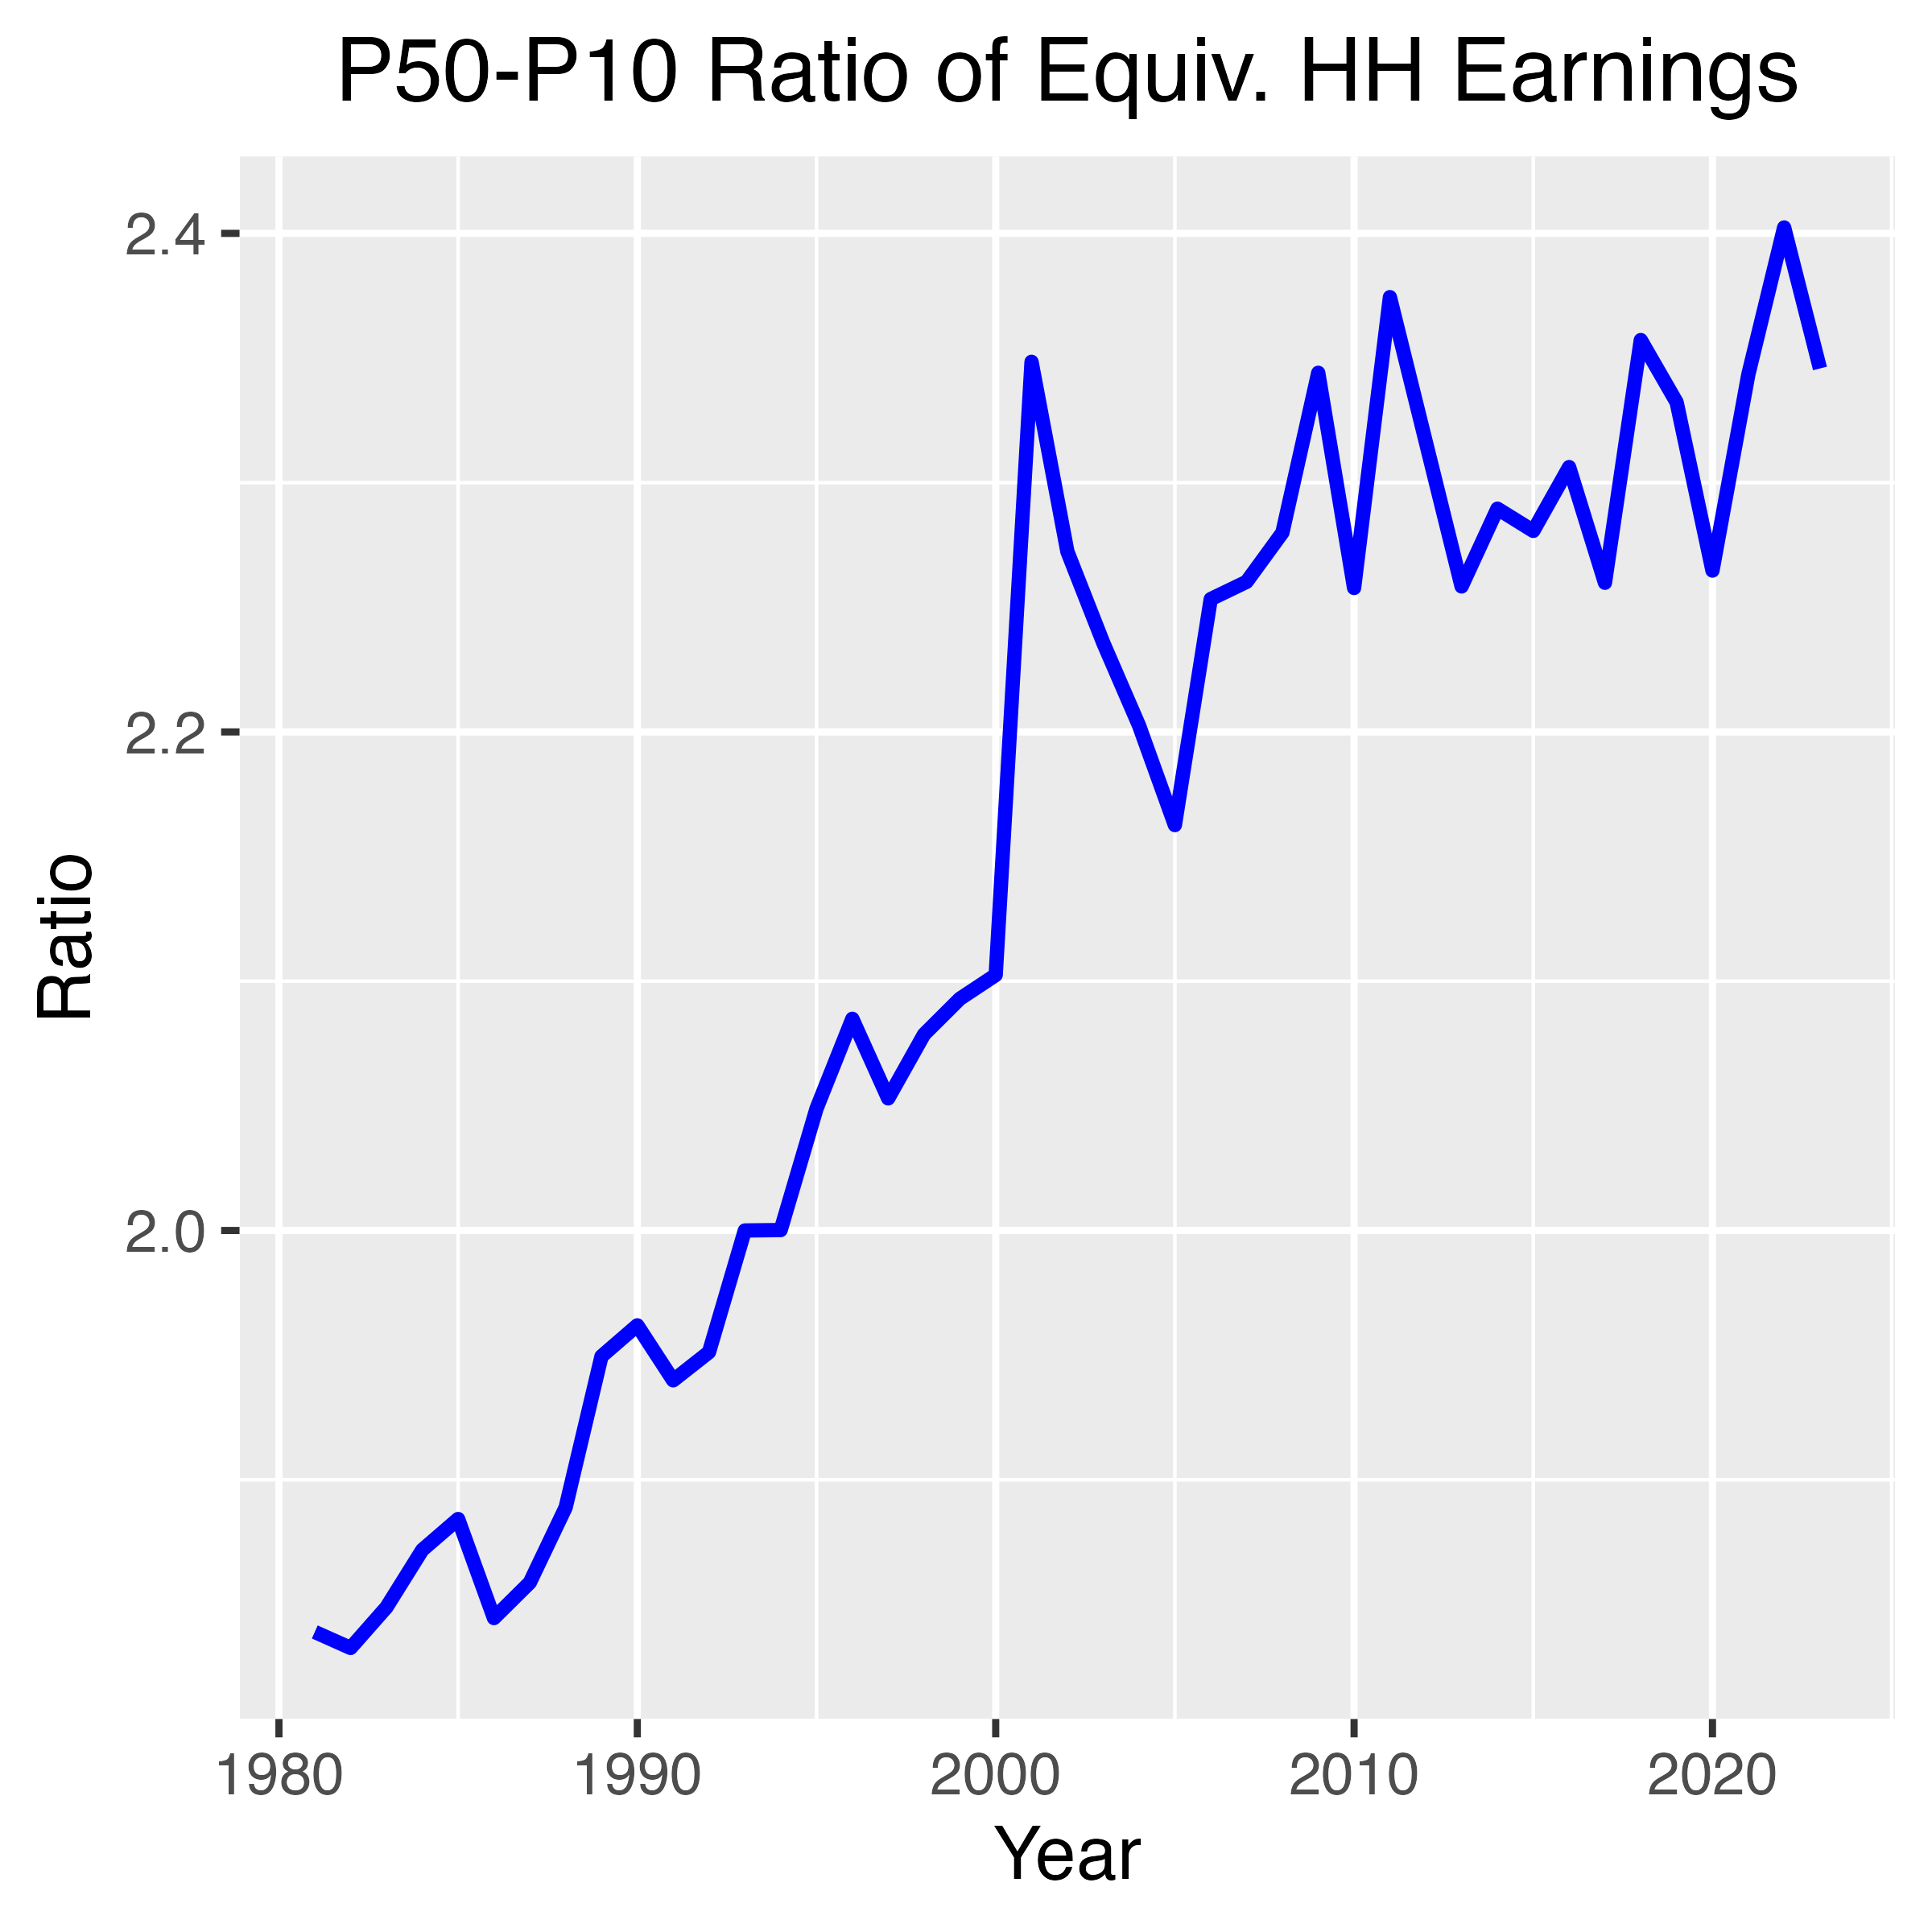
\includegraphics[width=\textwidth]{figures/Fig_1/Fig_1c_P50_P10_Earnings.png}
        \label{fig:earnings_inequality_P50_P10}
    \end{subfigure}
    \begin{subfigure}[t]{0.475\textwidth}
        \centering
        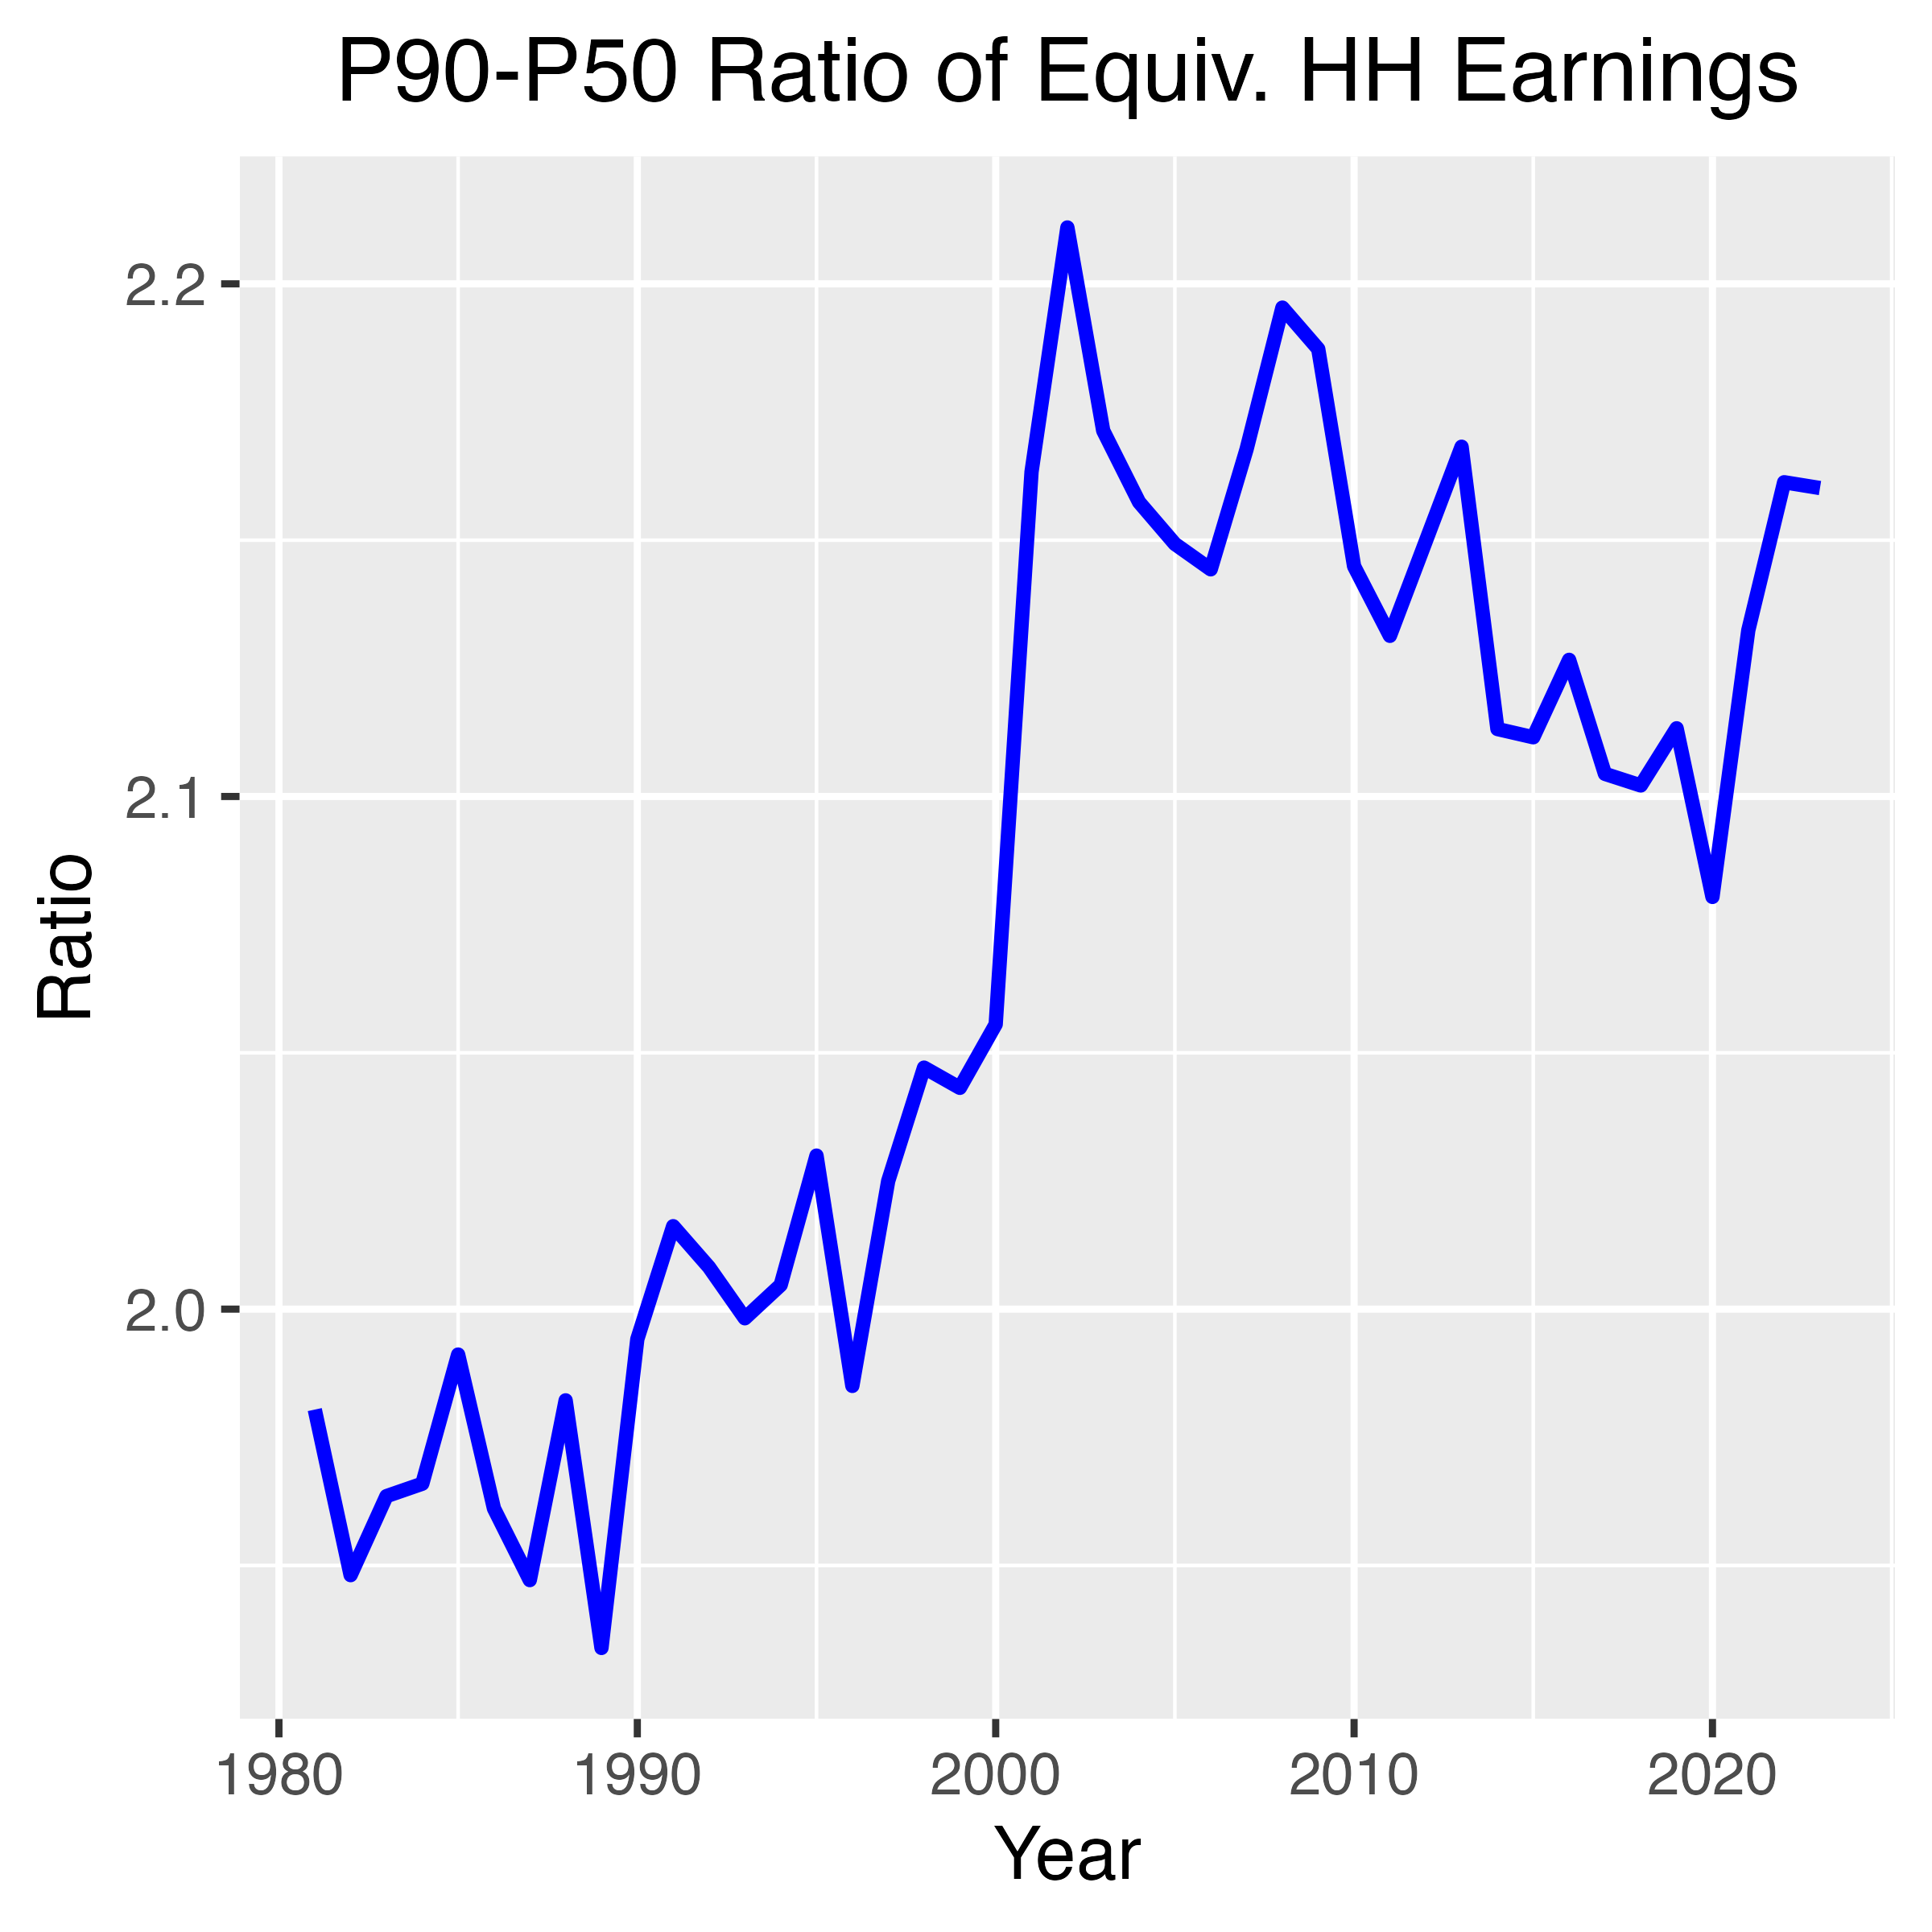
\includegraphics[width=\textwidth]{figures/Fig_1/Fig_1d_P90_P50_Earnings.png}
        \label{fig:earnings_inequality_P90_P50}
    \end{subfigure}
    \caption{Various Measures of Household Earnings Inequality}
    \label{fig:earnings_inequality}
\end{figure}

\subsection{Cyclical Dynamics of Earnings Inequality}

\begin{figure}
    \centering
    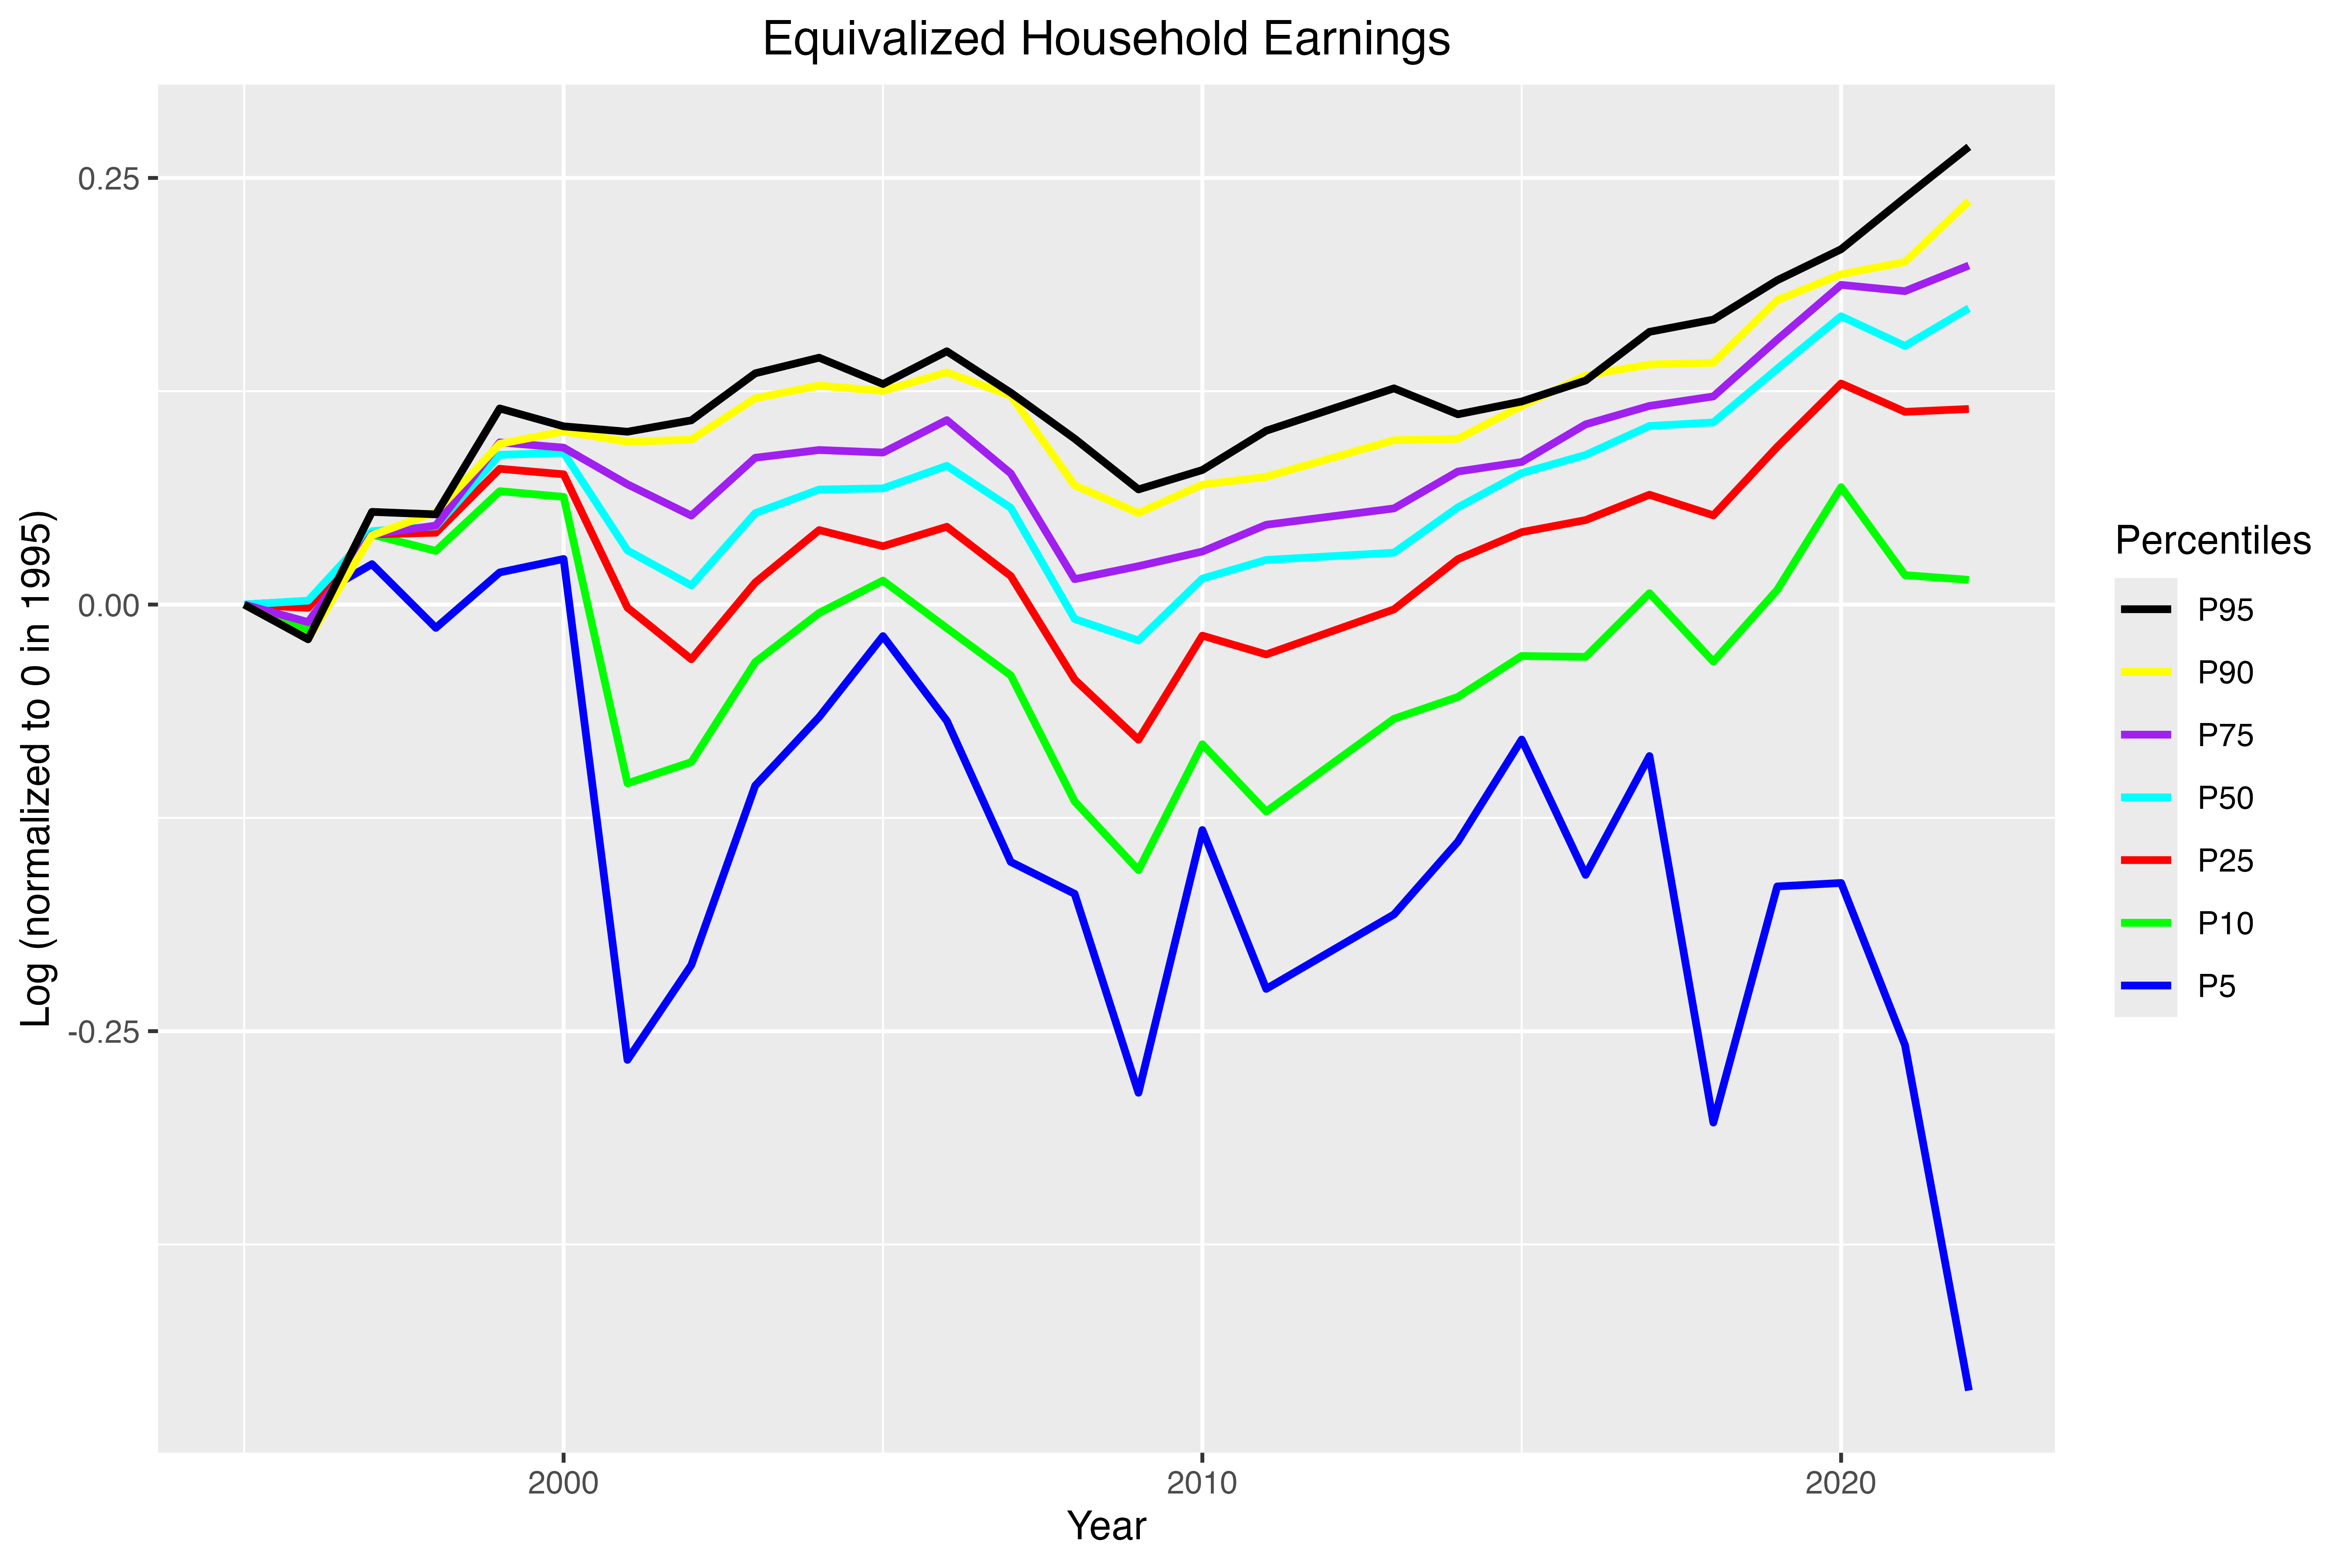
\includegraphics[width=0.95\textwidth]{figures/Fig_2/Fig_2_percentiles_a1995.png}
    \caption{Percentiles of the Household Earnings Distribution}
    \label{fig:earnings_inequality_cyclic}
\end{figure}

\subsection{From Individual to Household Inequality}

\begin{figure}
    \centering
    \begin{subfigure}[t]{0.475\textwidth}
        \centering
        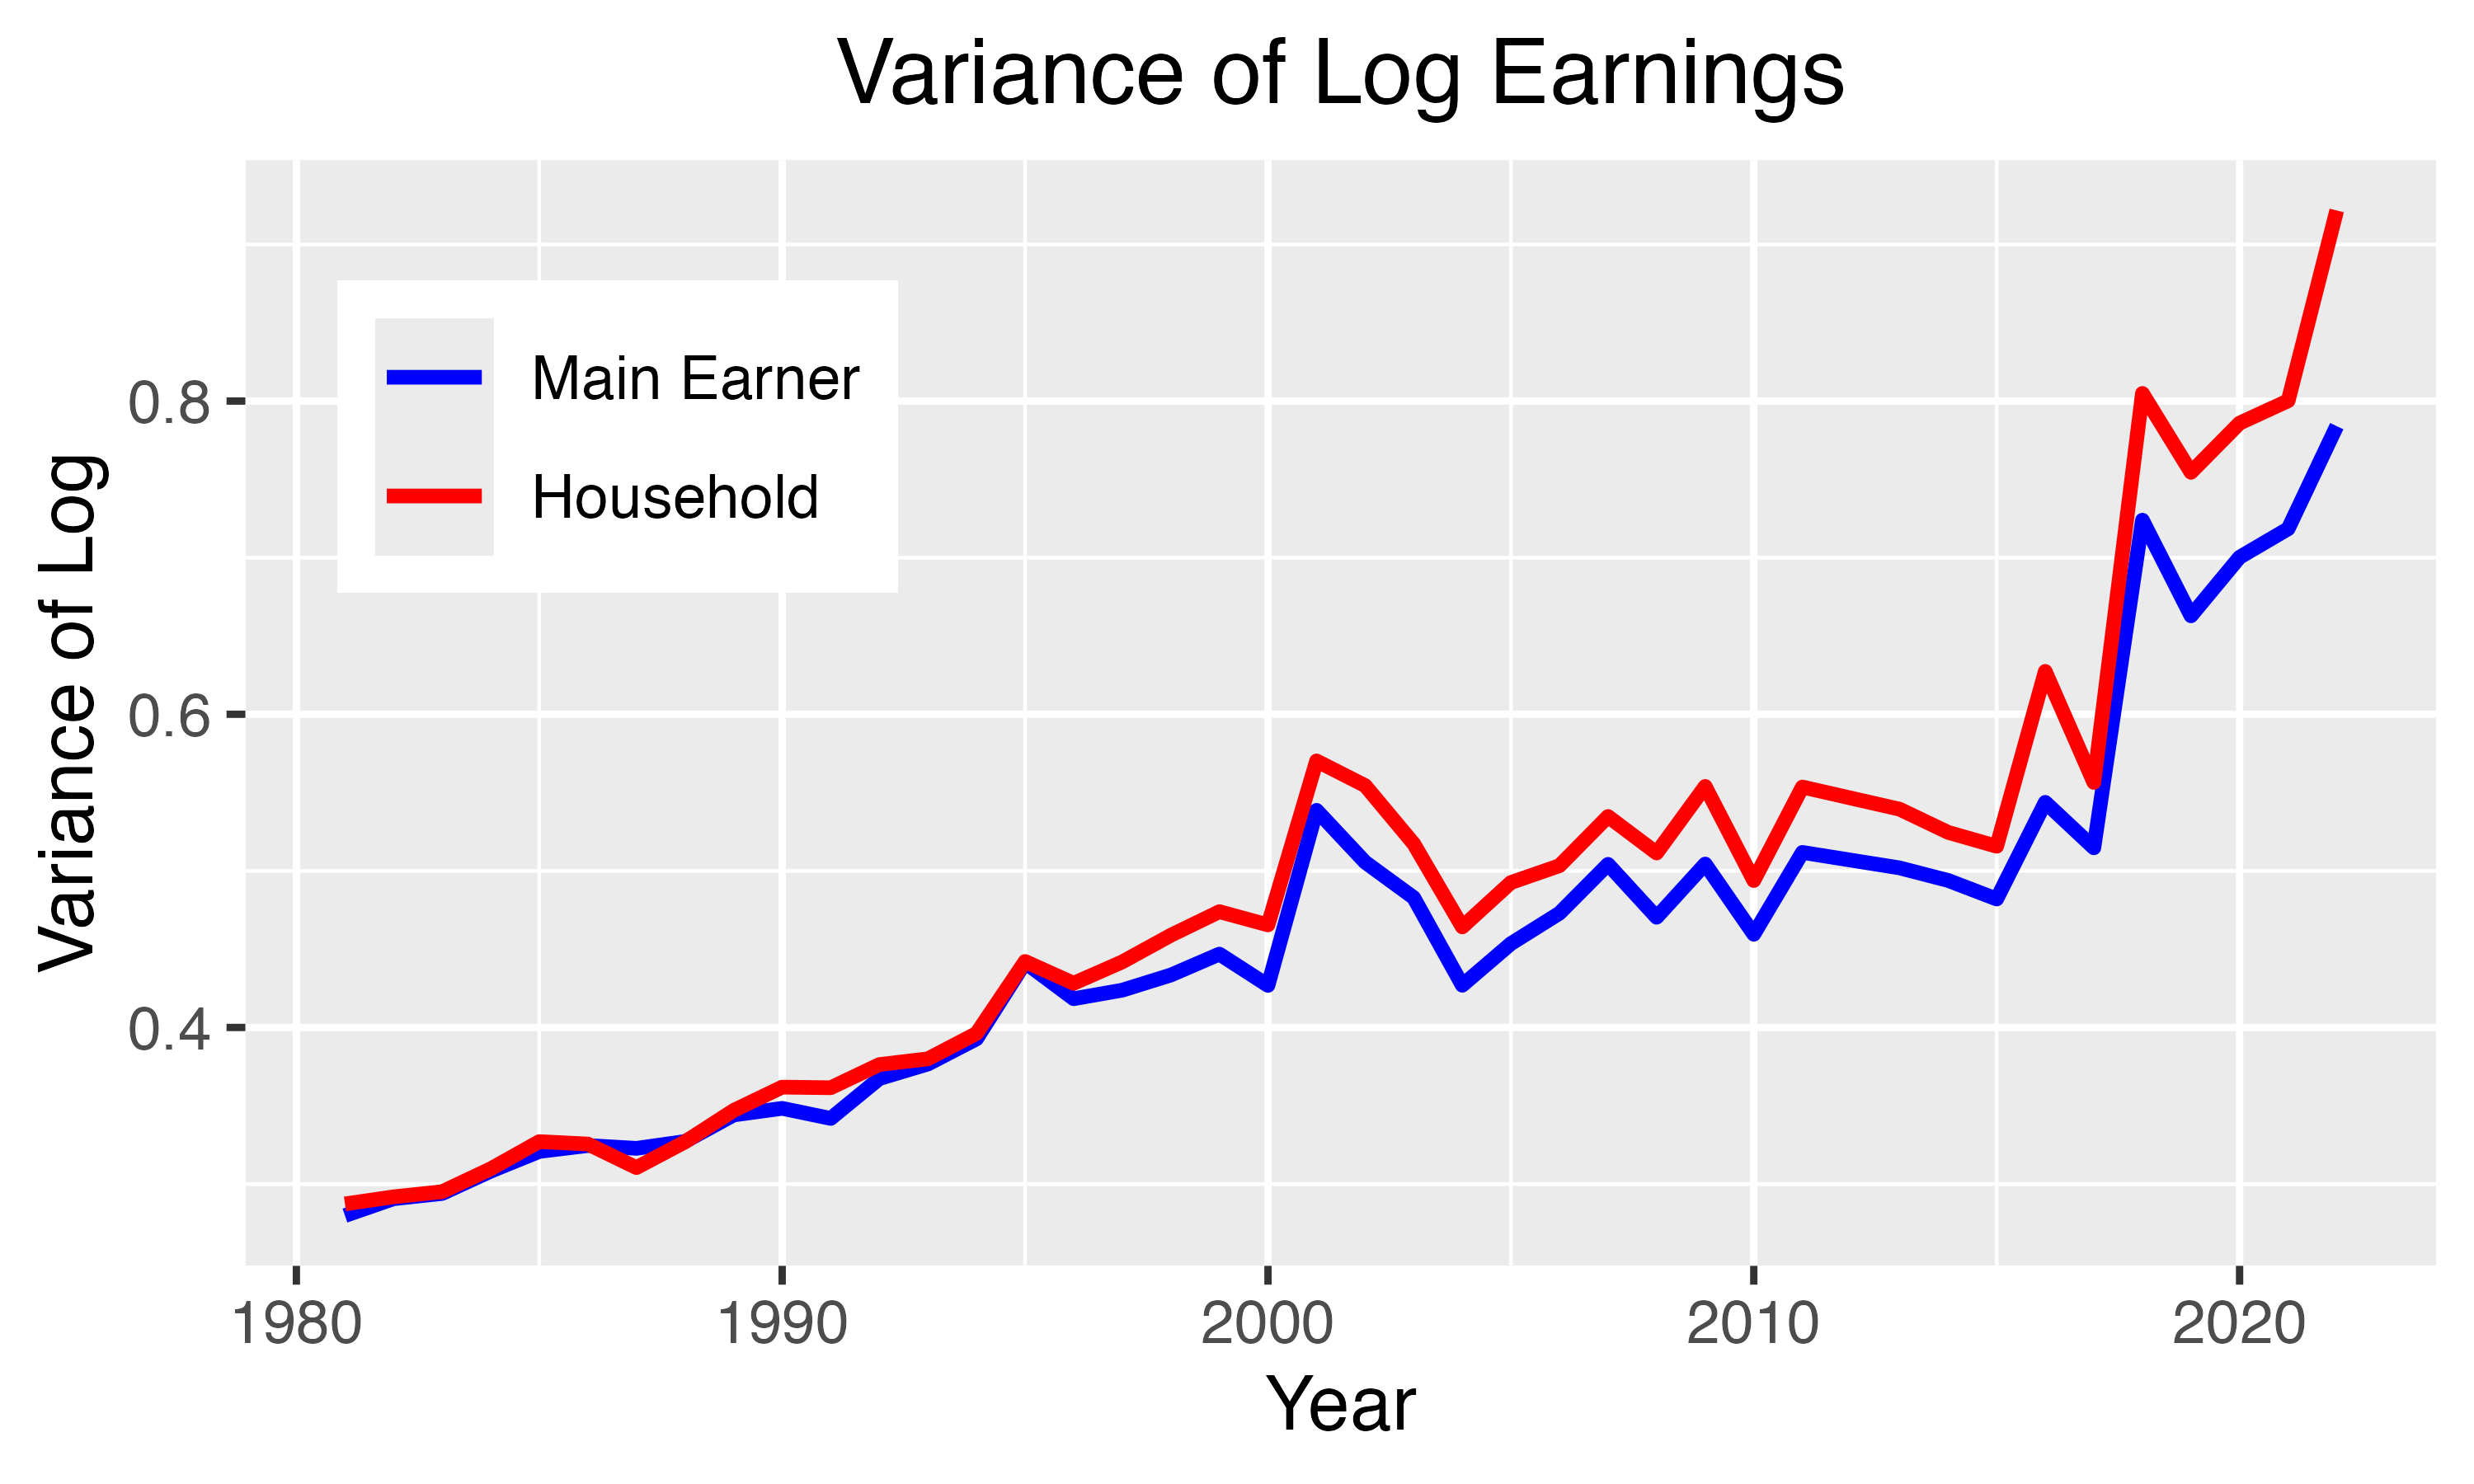
\includegraphics[width=\textwidth]{figures/Fig_3/Fig_3a_Var_indHH.png}
        \label{fig:Indi_to_HH_Var}
    \end{subfigure}
    \begin{subfigure}[t]{0.475\textwidth}
        \centering
        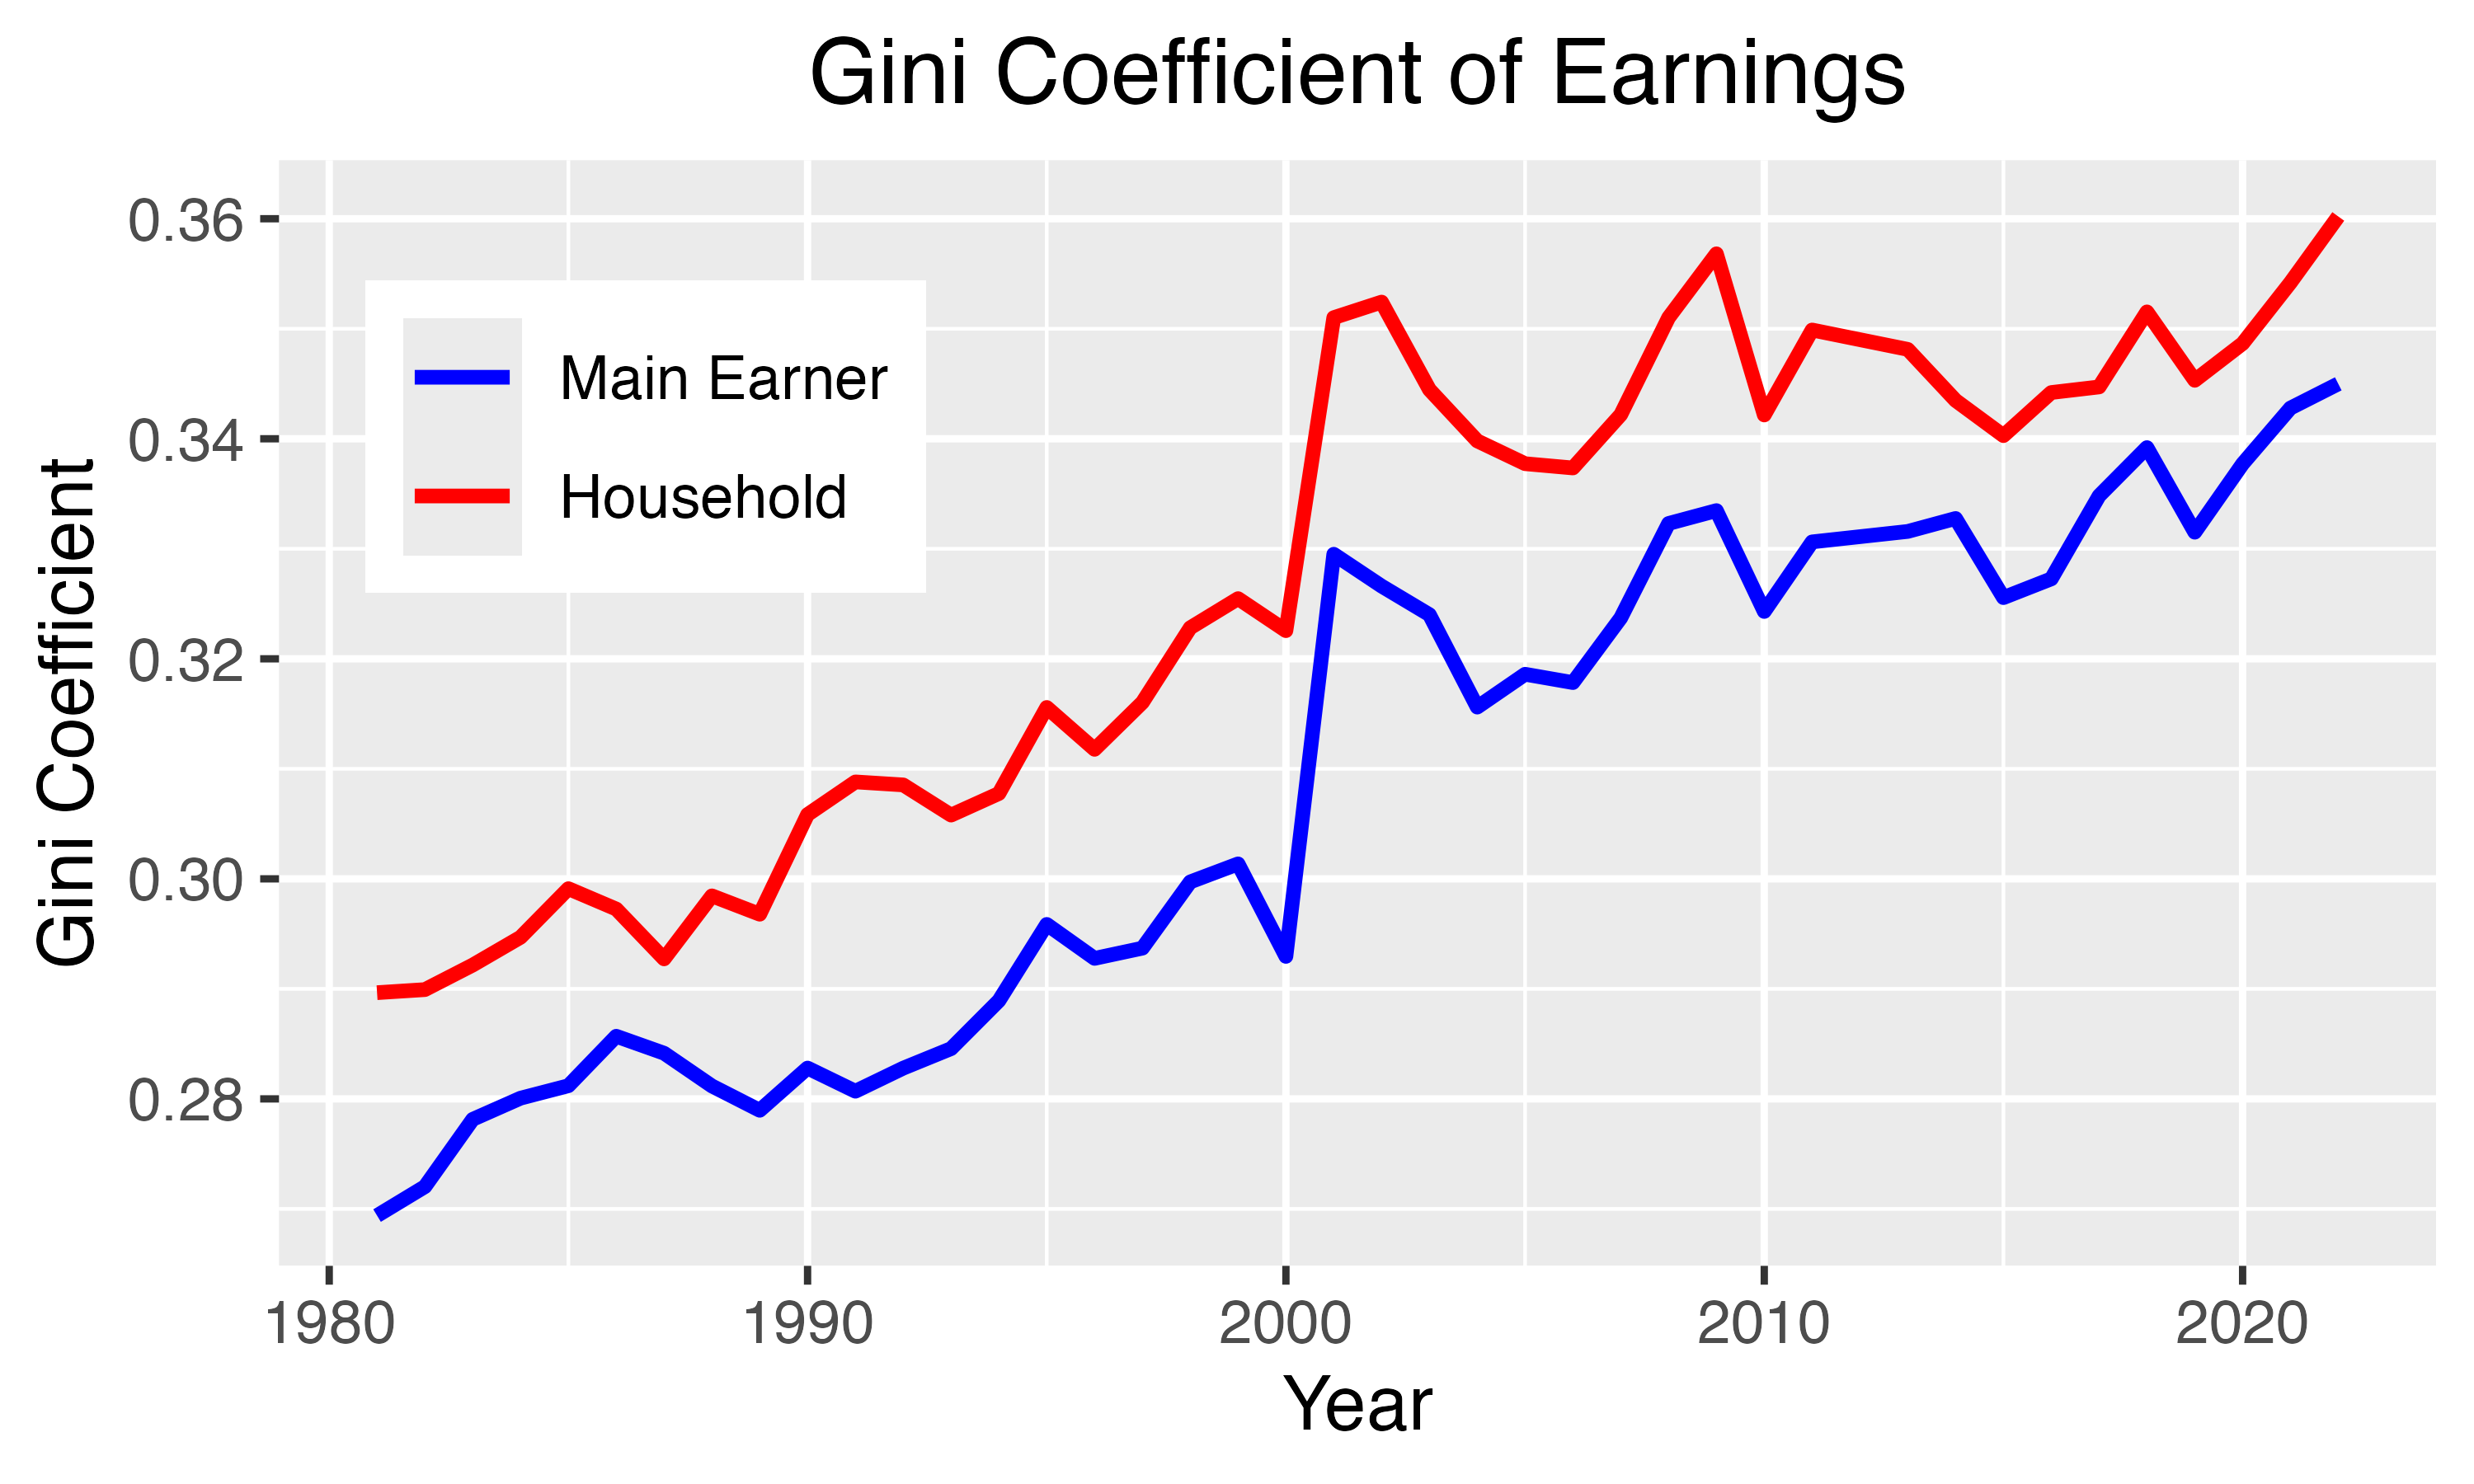
\includegraphics[width=\textwidth]{figures/Fig_3/Fig_3b_Gini_indHH.png}
        \label{fig:Indi_to_HH_Gini}
    \end{subfigure}
    \begin{subfigure}[t]{0.475\textwidth}
        \centering
        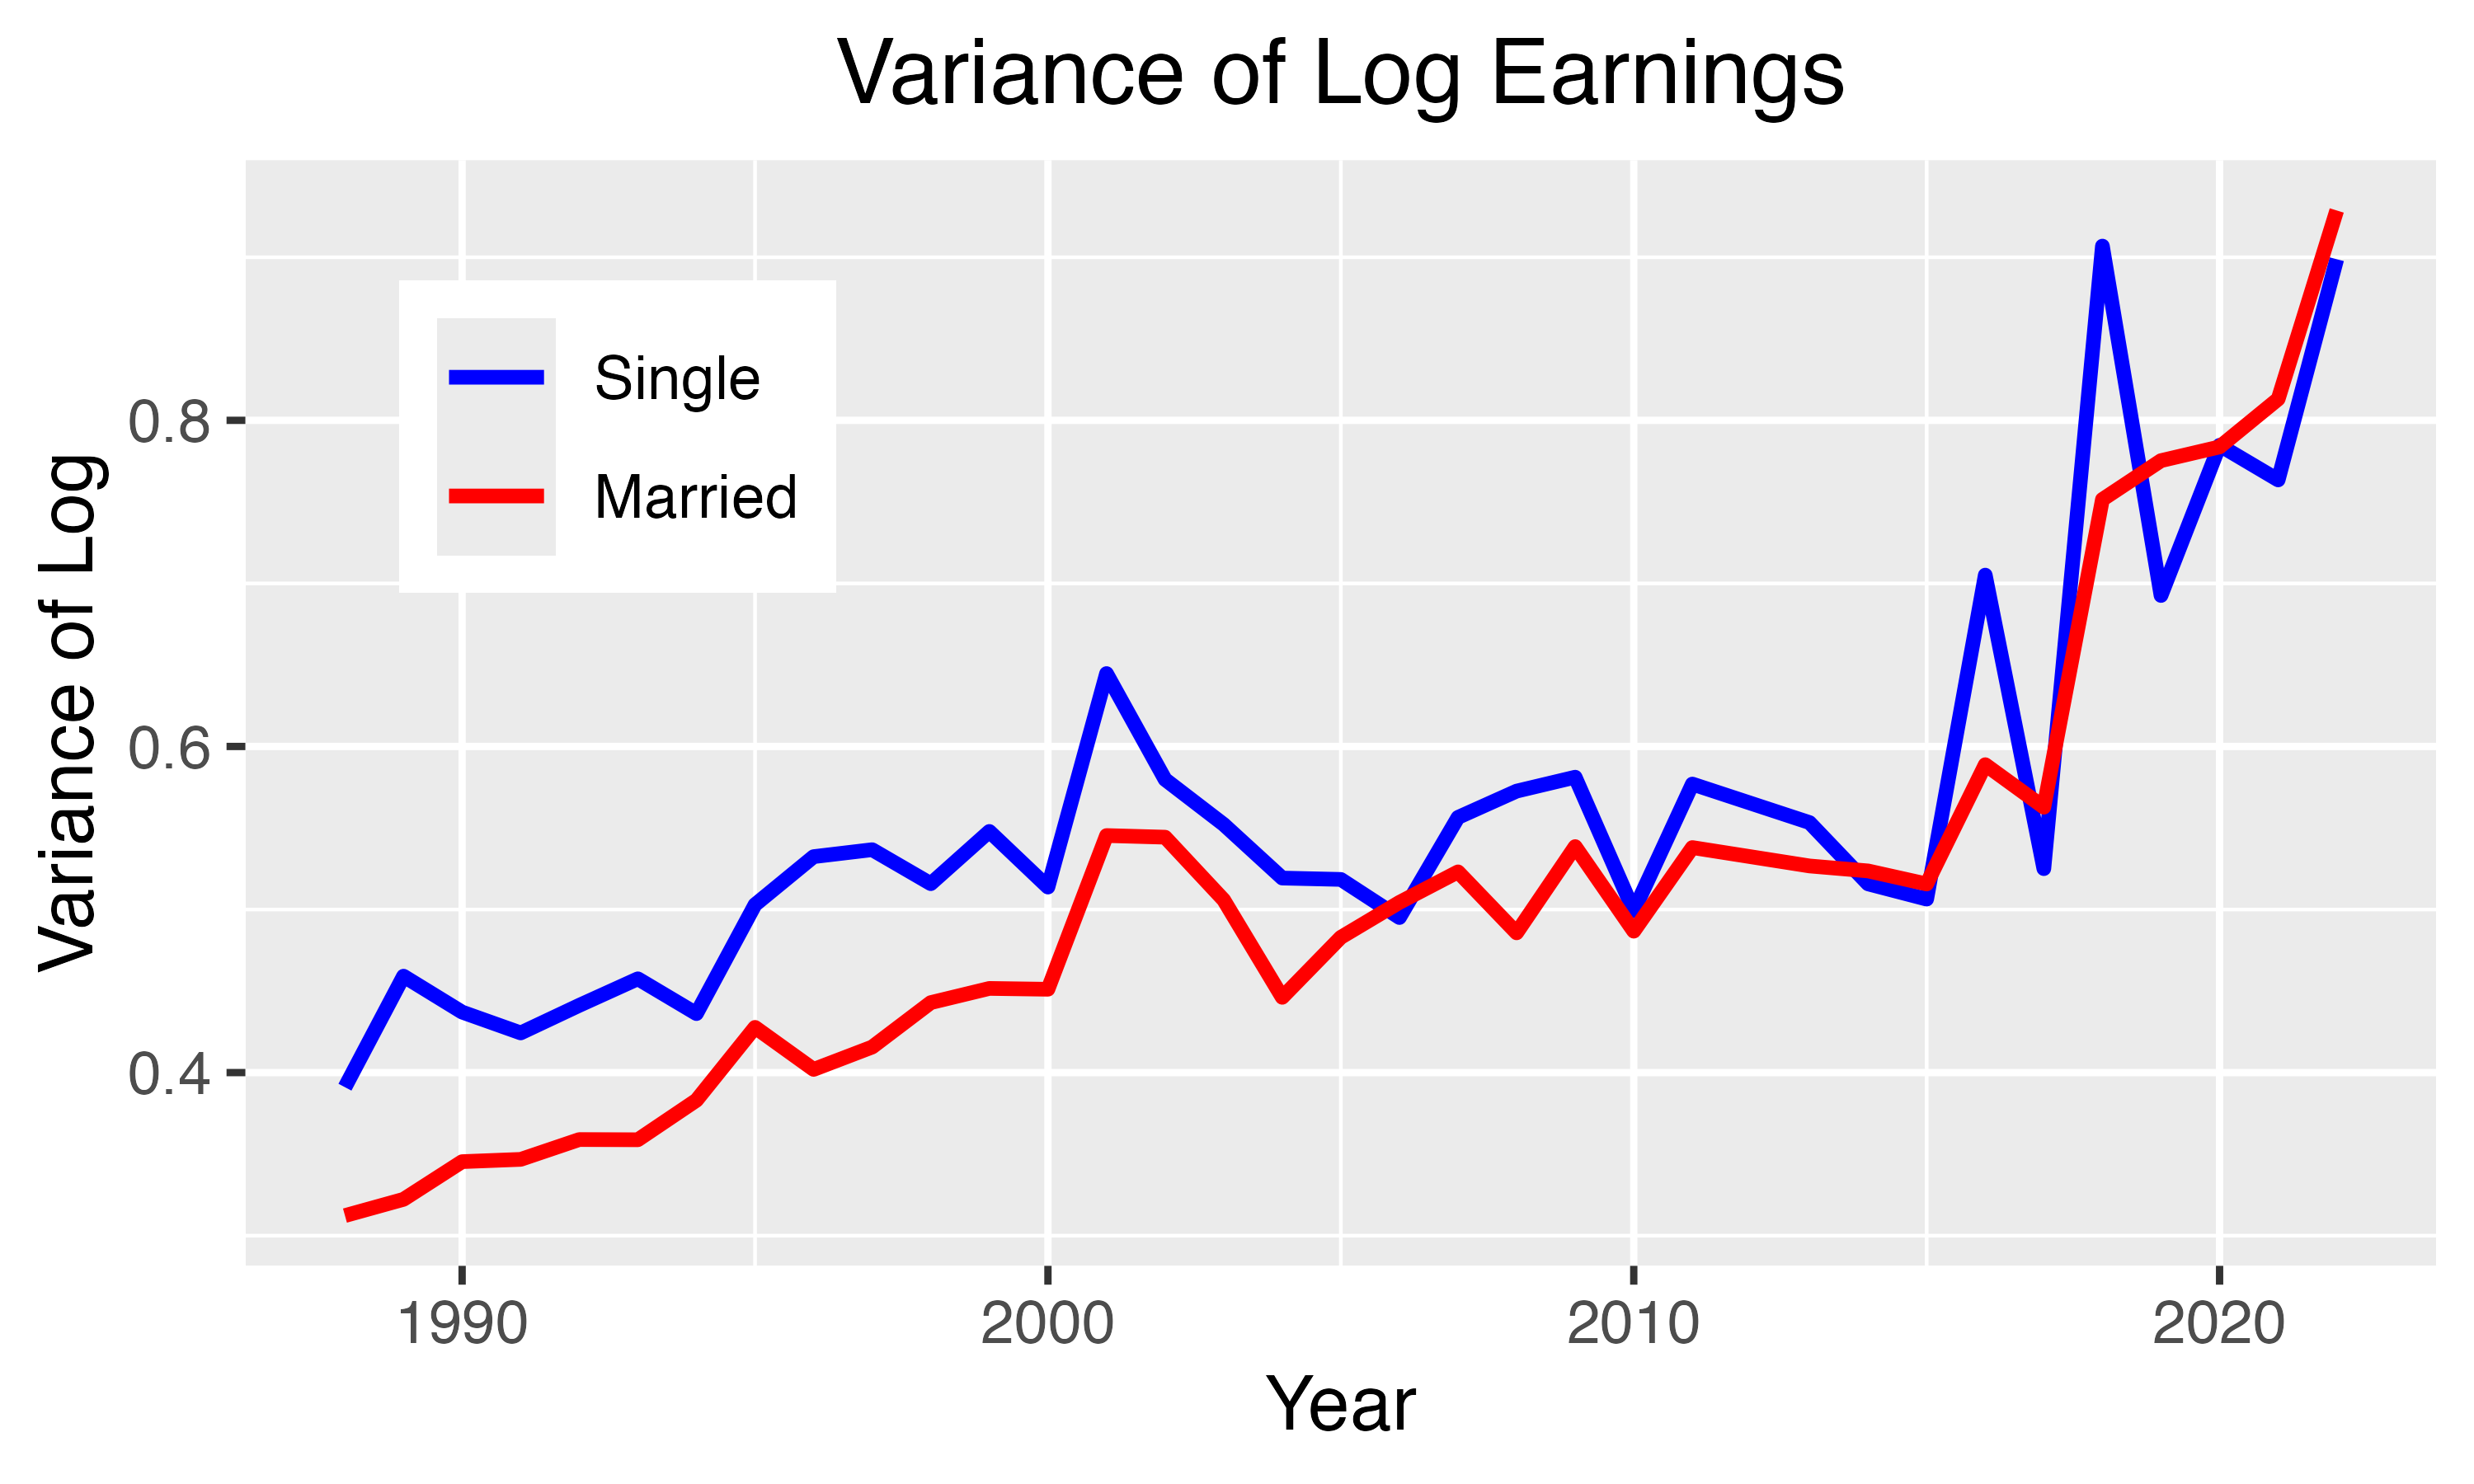
\includegraphics[width=\textwidth]{figures/Fig_3/Fig_3c_Var_single.png}
        \label{fig:Indi_to_HH_Var_single}
    \end{subfigure}
    \begin{subfigure}[t]{0.475\textwidth}
        \centering
        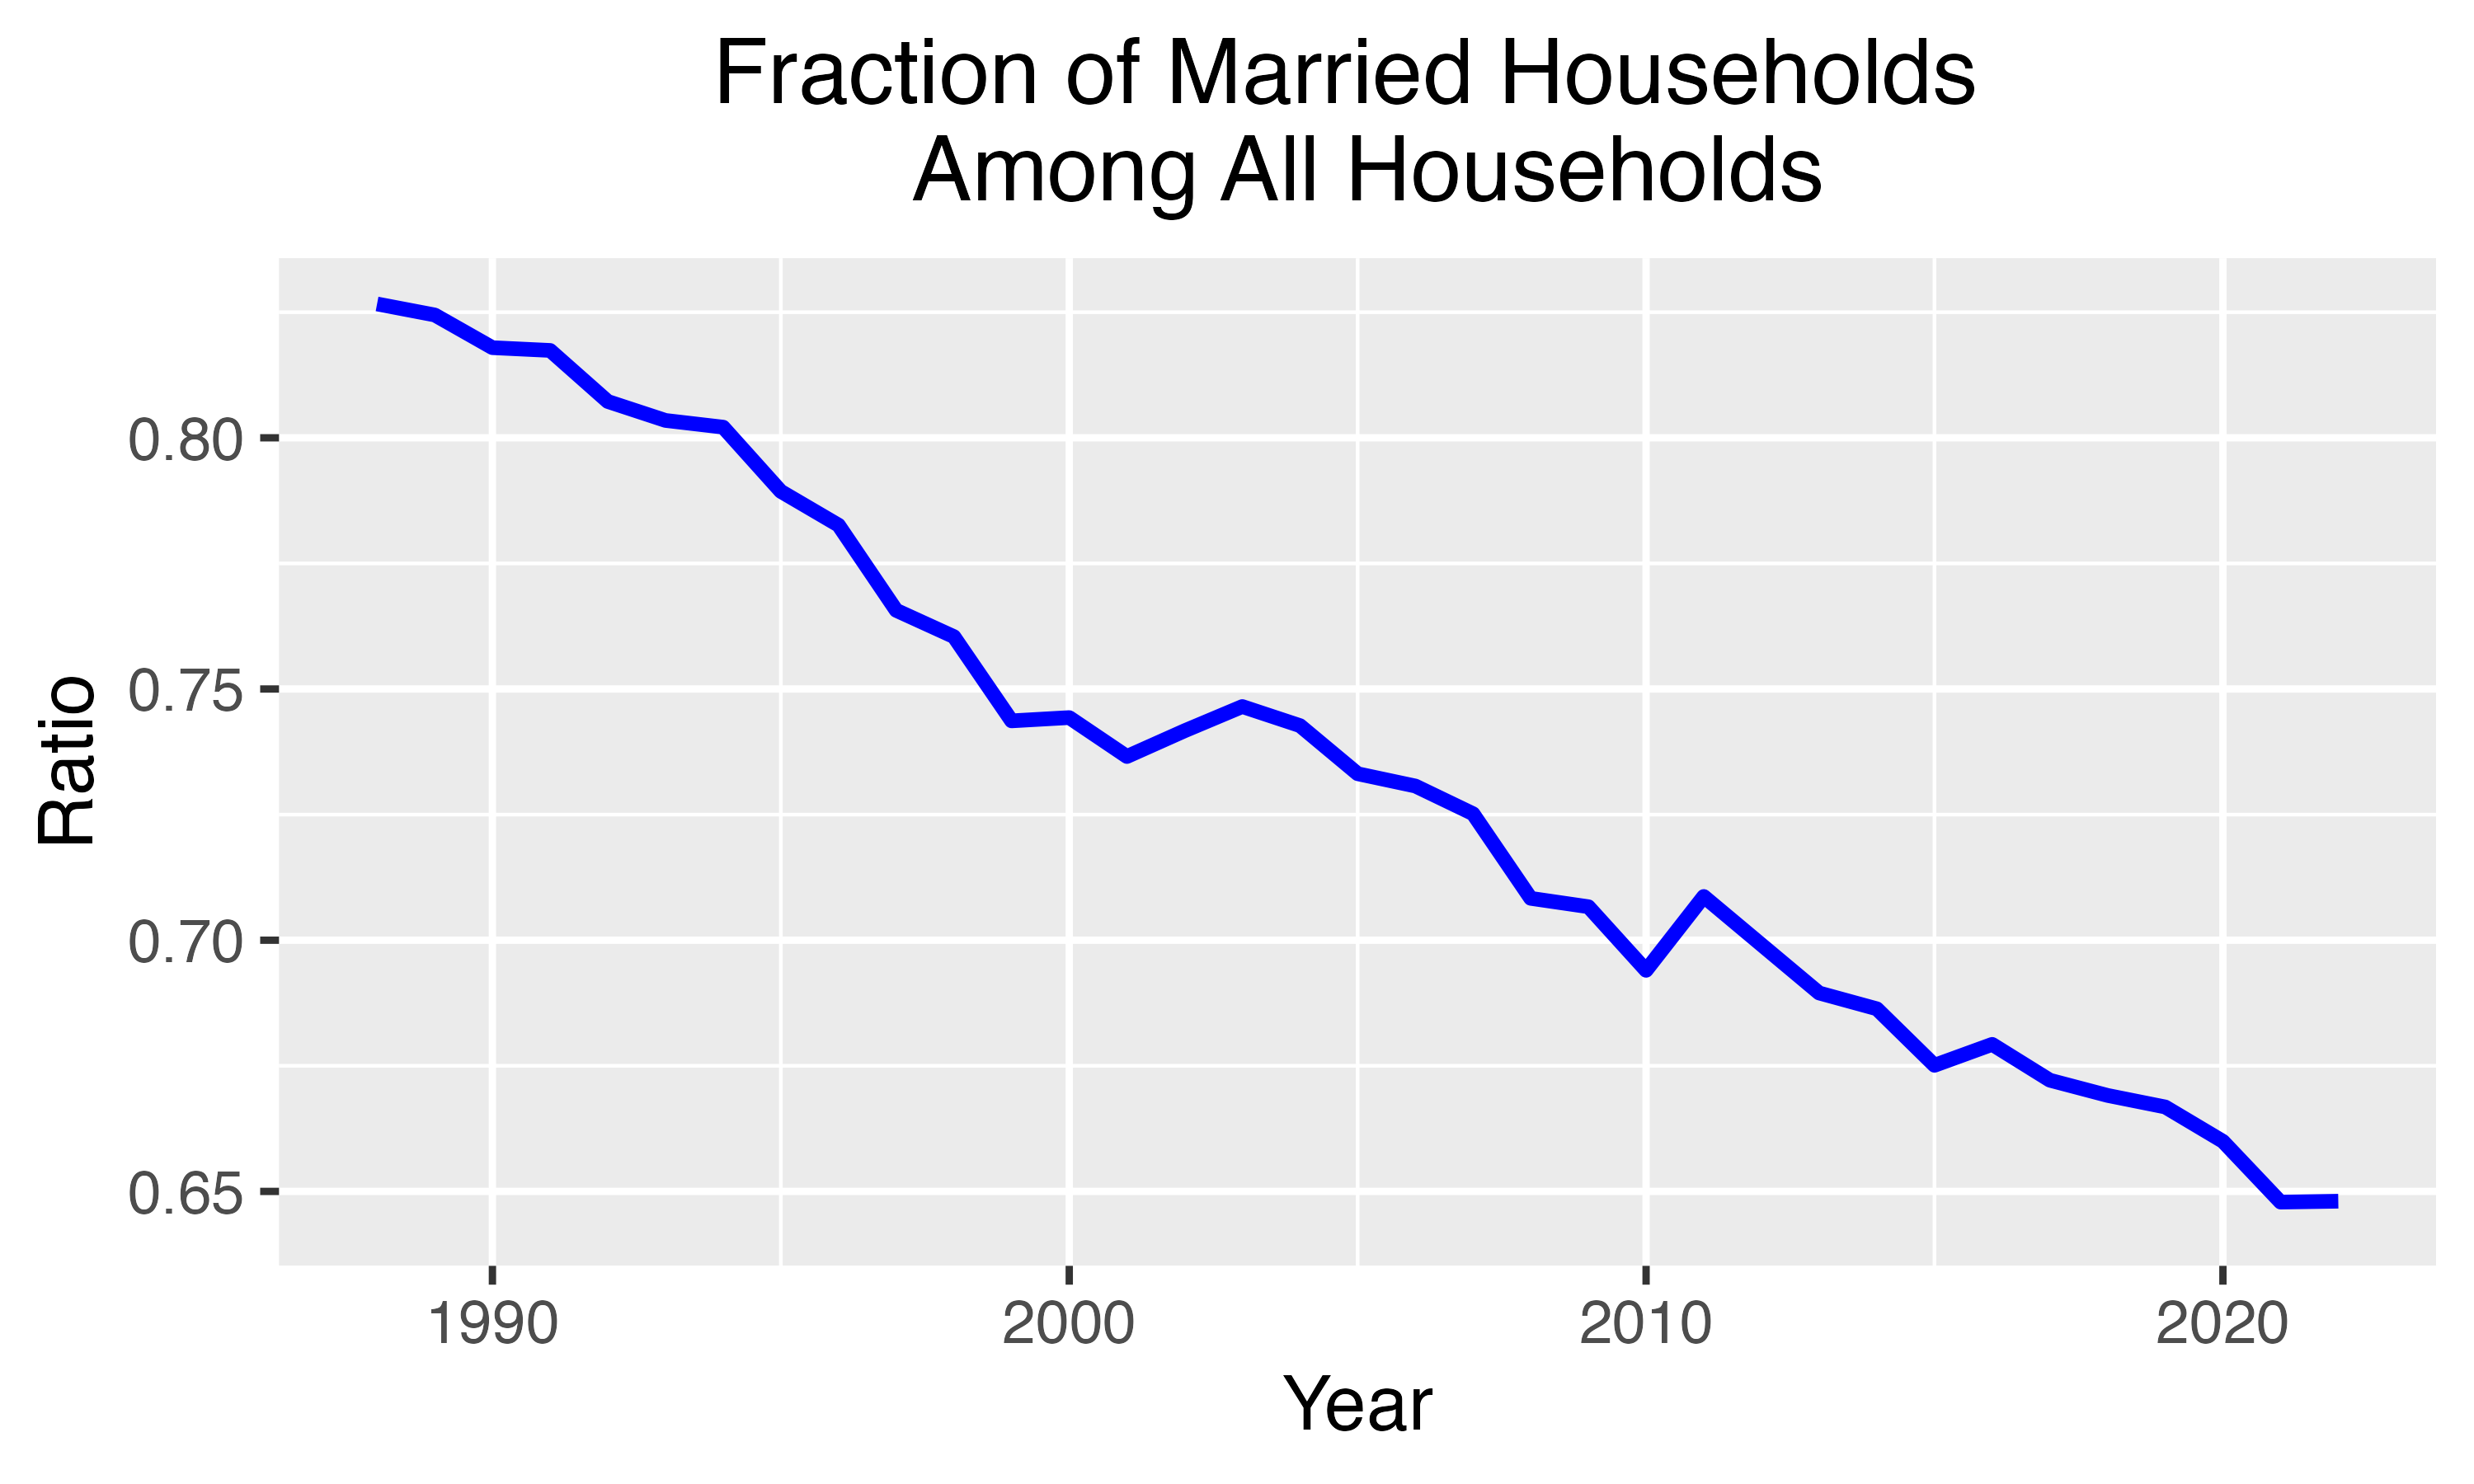
\includegraphics[width=\textwidth]{figures/Fig_3/Fig_3d_married_ratio.png}
        \label{fig:Indi_to_HH_married_ratio}
    \end{subfigure}
    \begin{subfigure}[t]{0.475\textwidth}
        \centering
        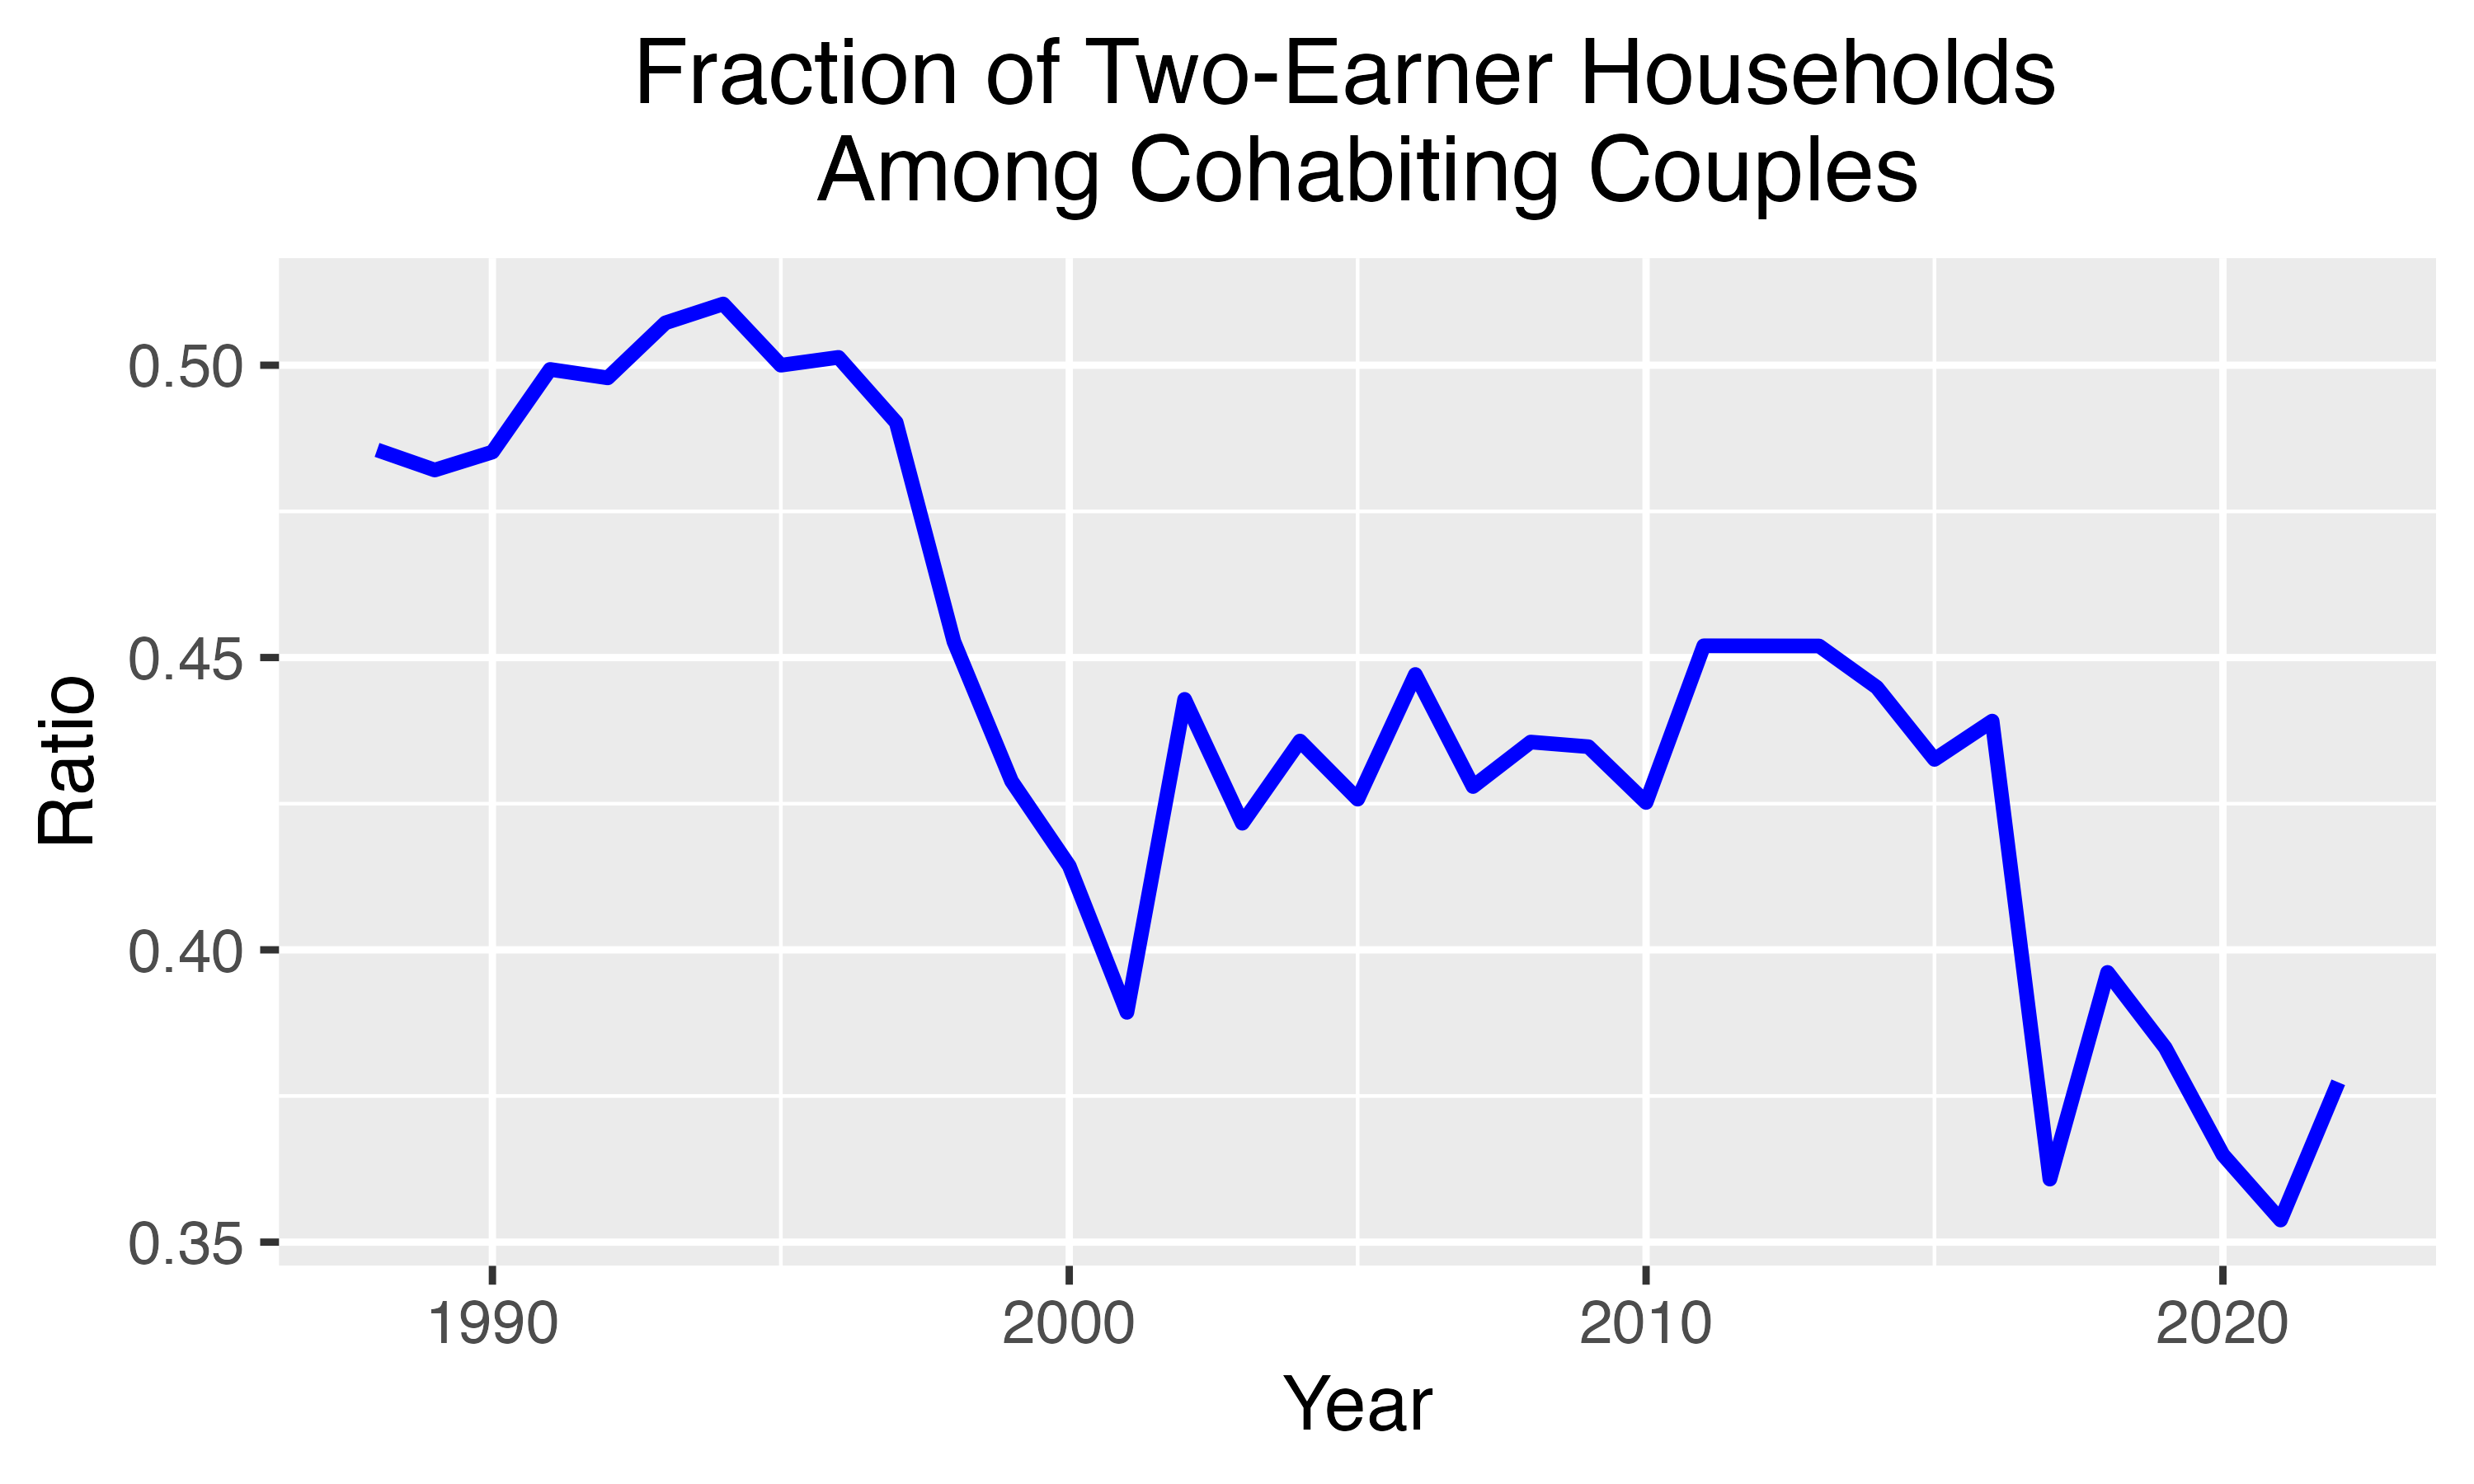
\includegraphics[width=\textwidth]{figures/Fig_3/Fig_3e_two_earner_ratio.png}
        \label{fig:Indi_to_HH_two_earner_ratio}
    \end{subfigure}
    \begin{subfigure}[t]{0.475\textwidth}
        \centering
        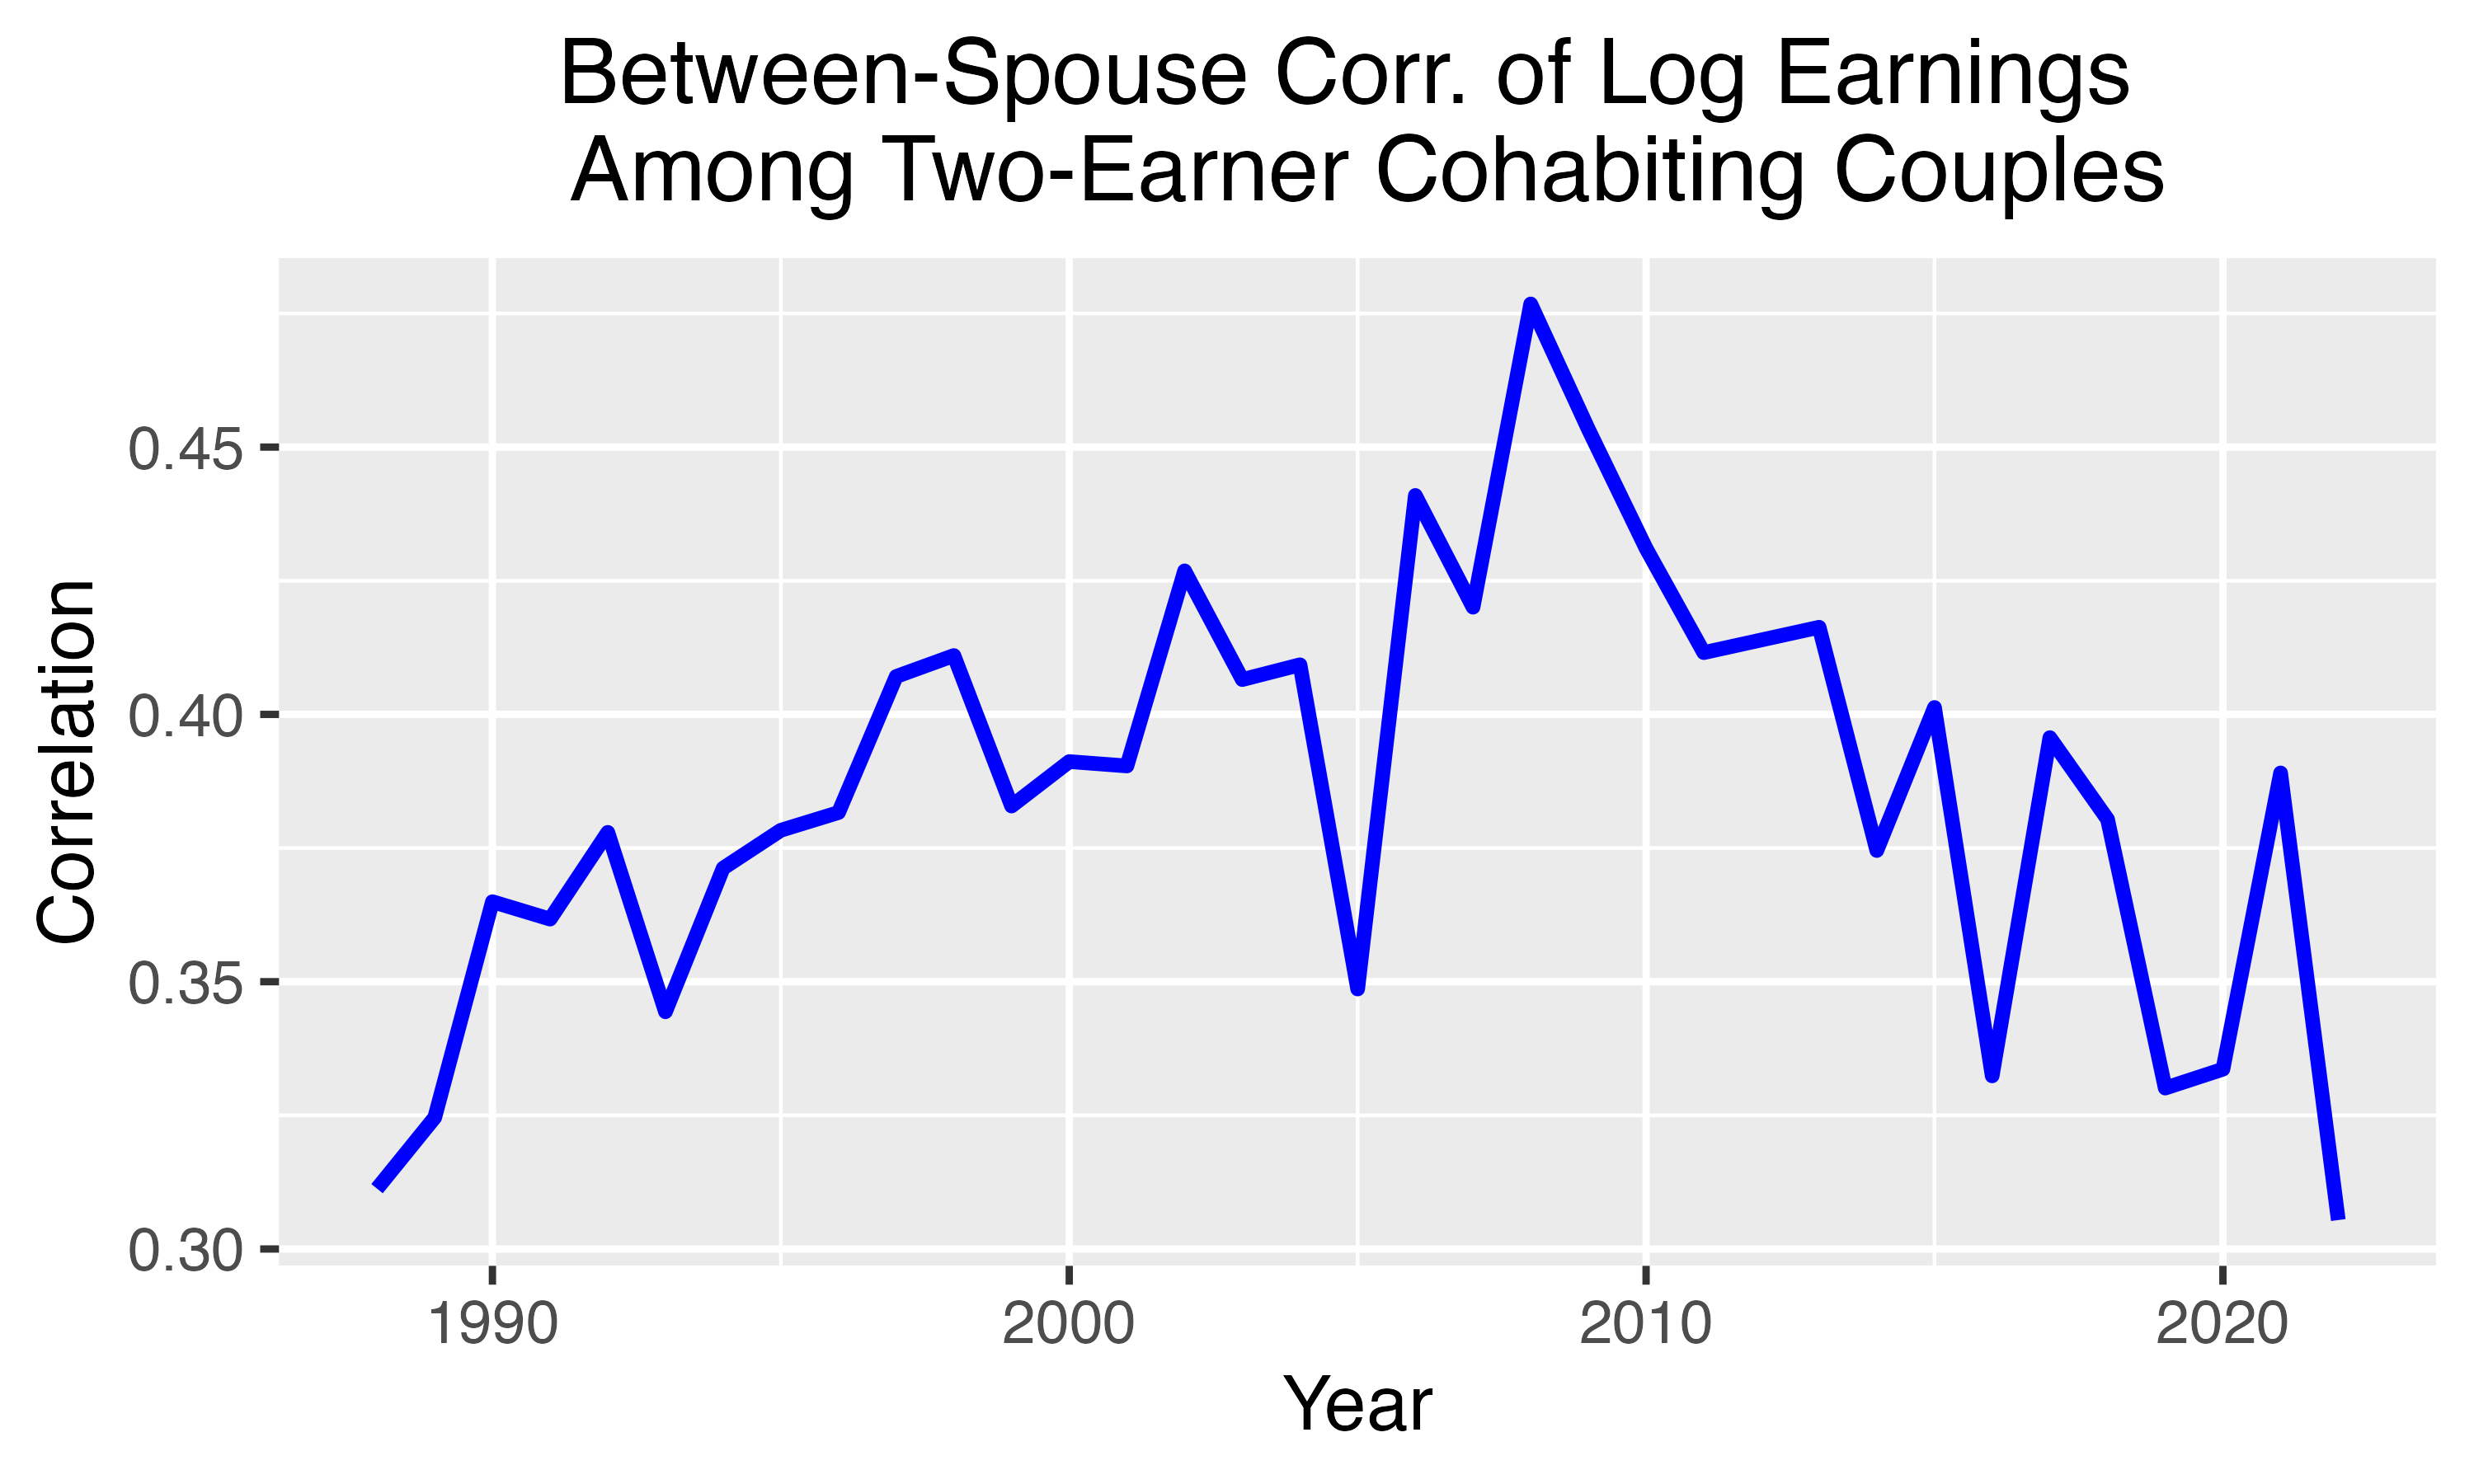
\includegraphics[width=\textwidth]{figures/Fig_3/Fig_3f_correlation.png}
        \label{fig:Indi_to_HH_correlation}
    \end{subfigure}
    \caption{Understanding the role of the Family for Earnings Inequality}
    \label{fig:Indi_to_HH}
\end{figure}

\subsection{Private Transfers and Asset Income}

\begin{figure}
    \centering
    \begin{subfigure}[t]{0.475\textwidth}
        \centering
        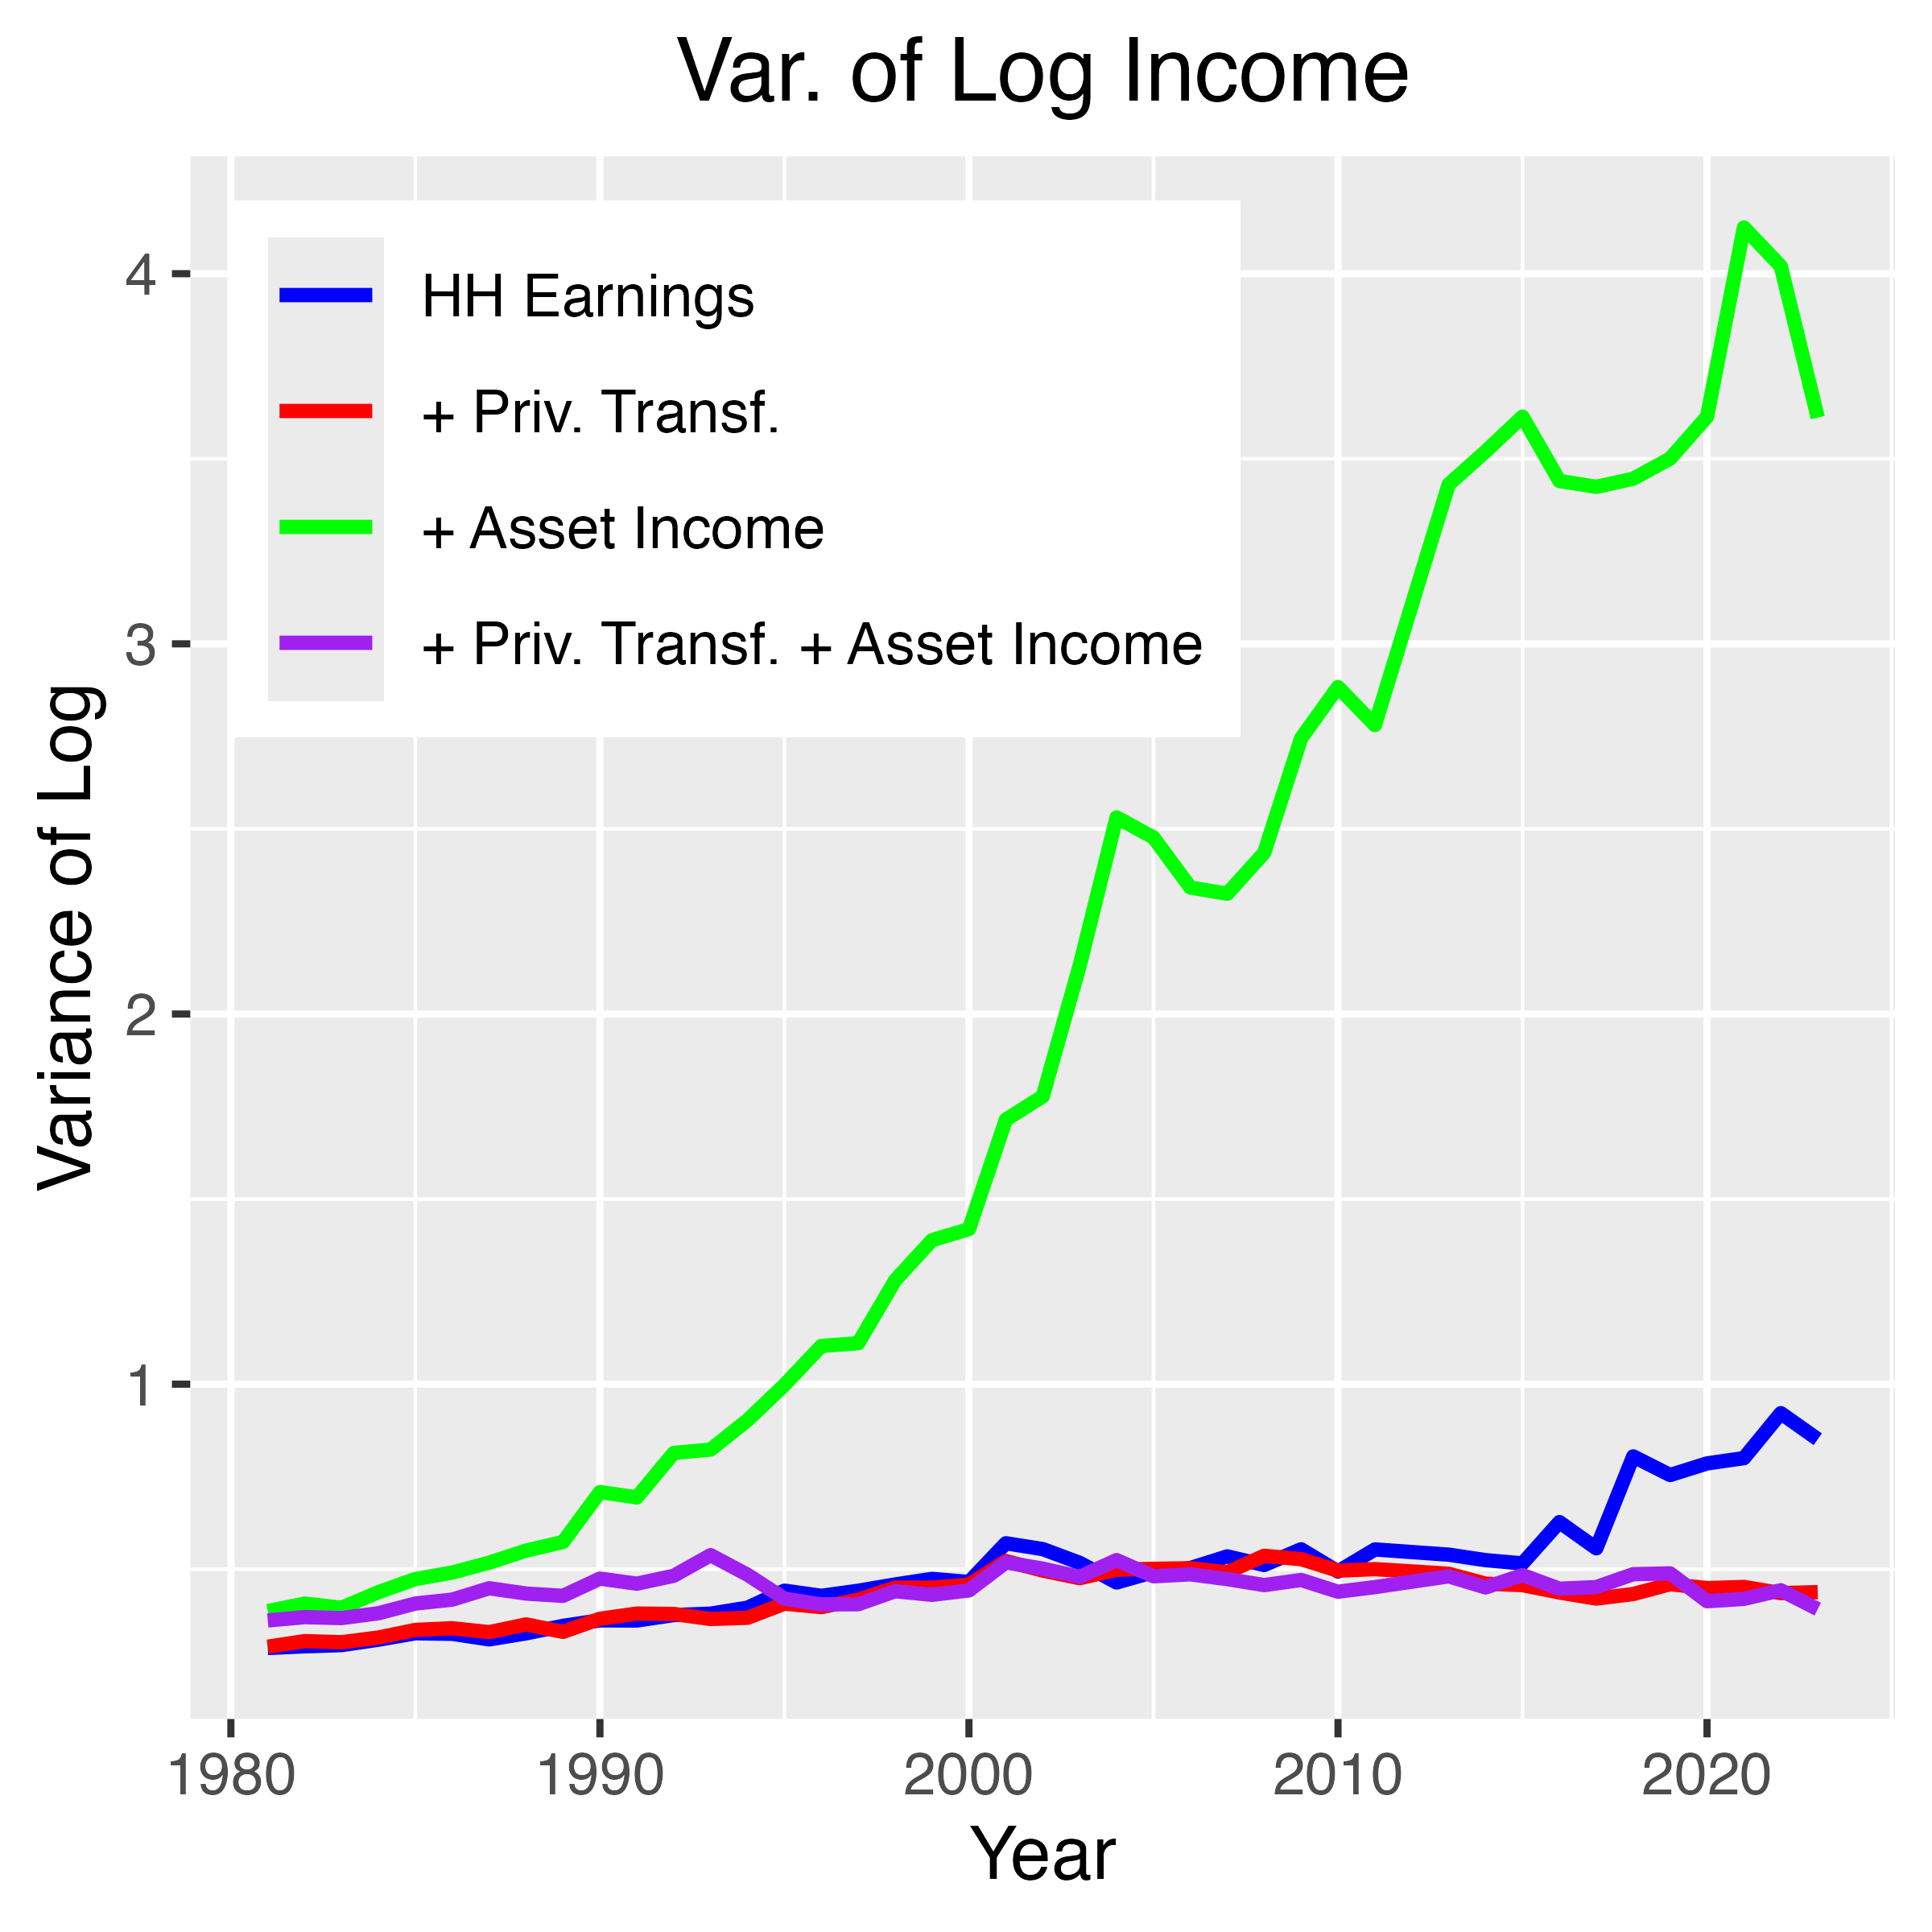
\includegraphics[width=\textwidth]{figures/Fig_4/Fig_4a_Var_inc.png}
        \label{fig:Trans_Asset_Var1}
    \end{subfigure}
    \begin{subfigure}[t]{0.475\textwidth}
        \centering
        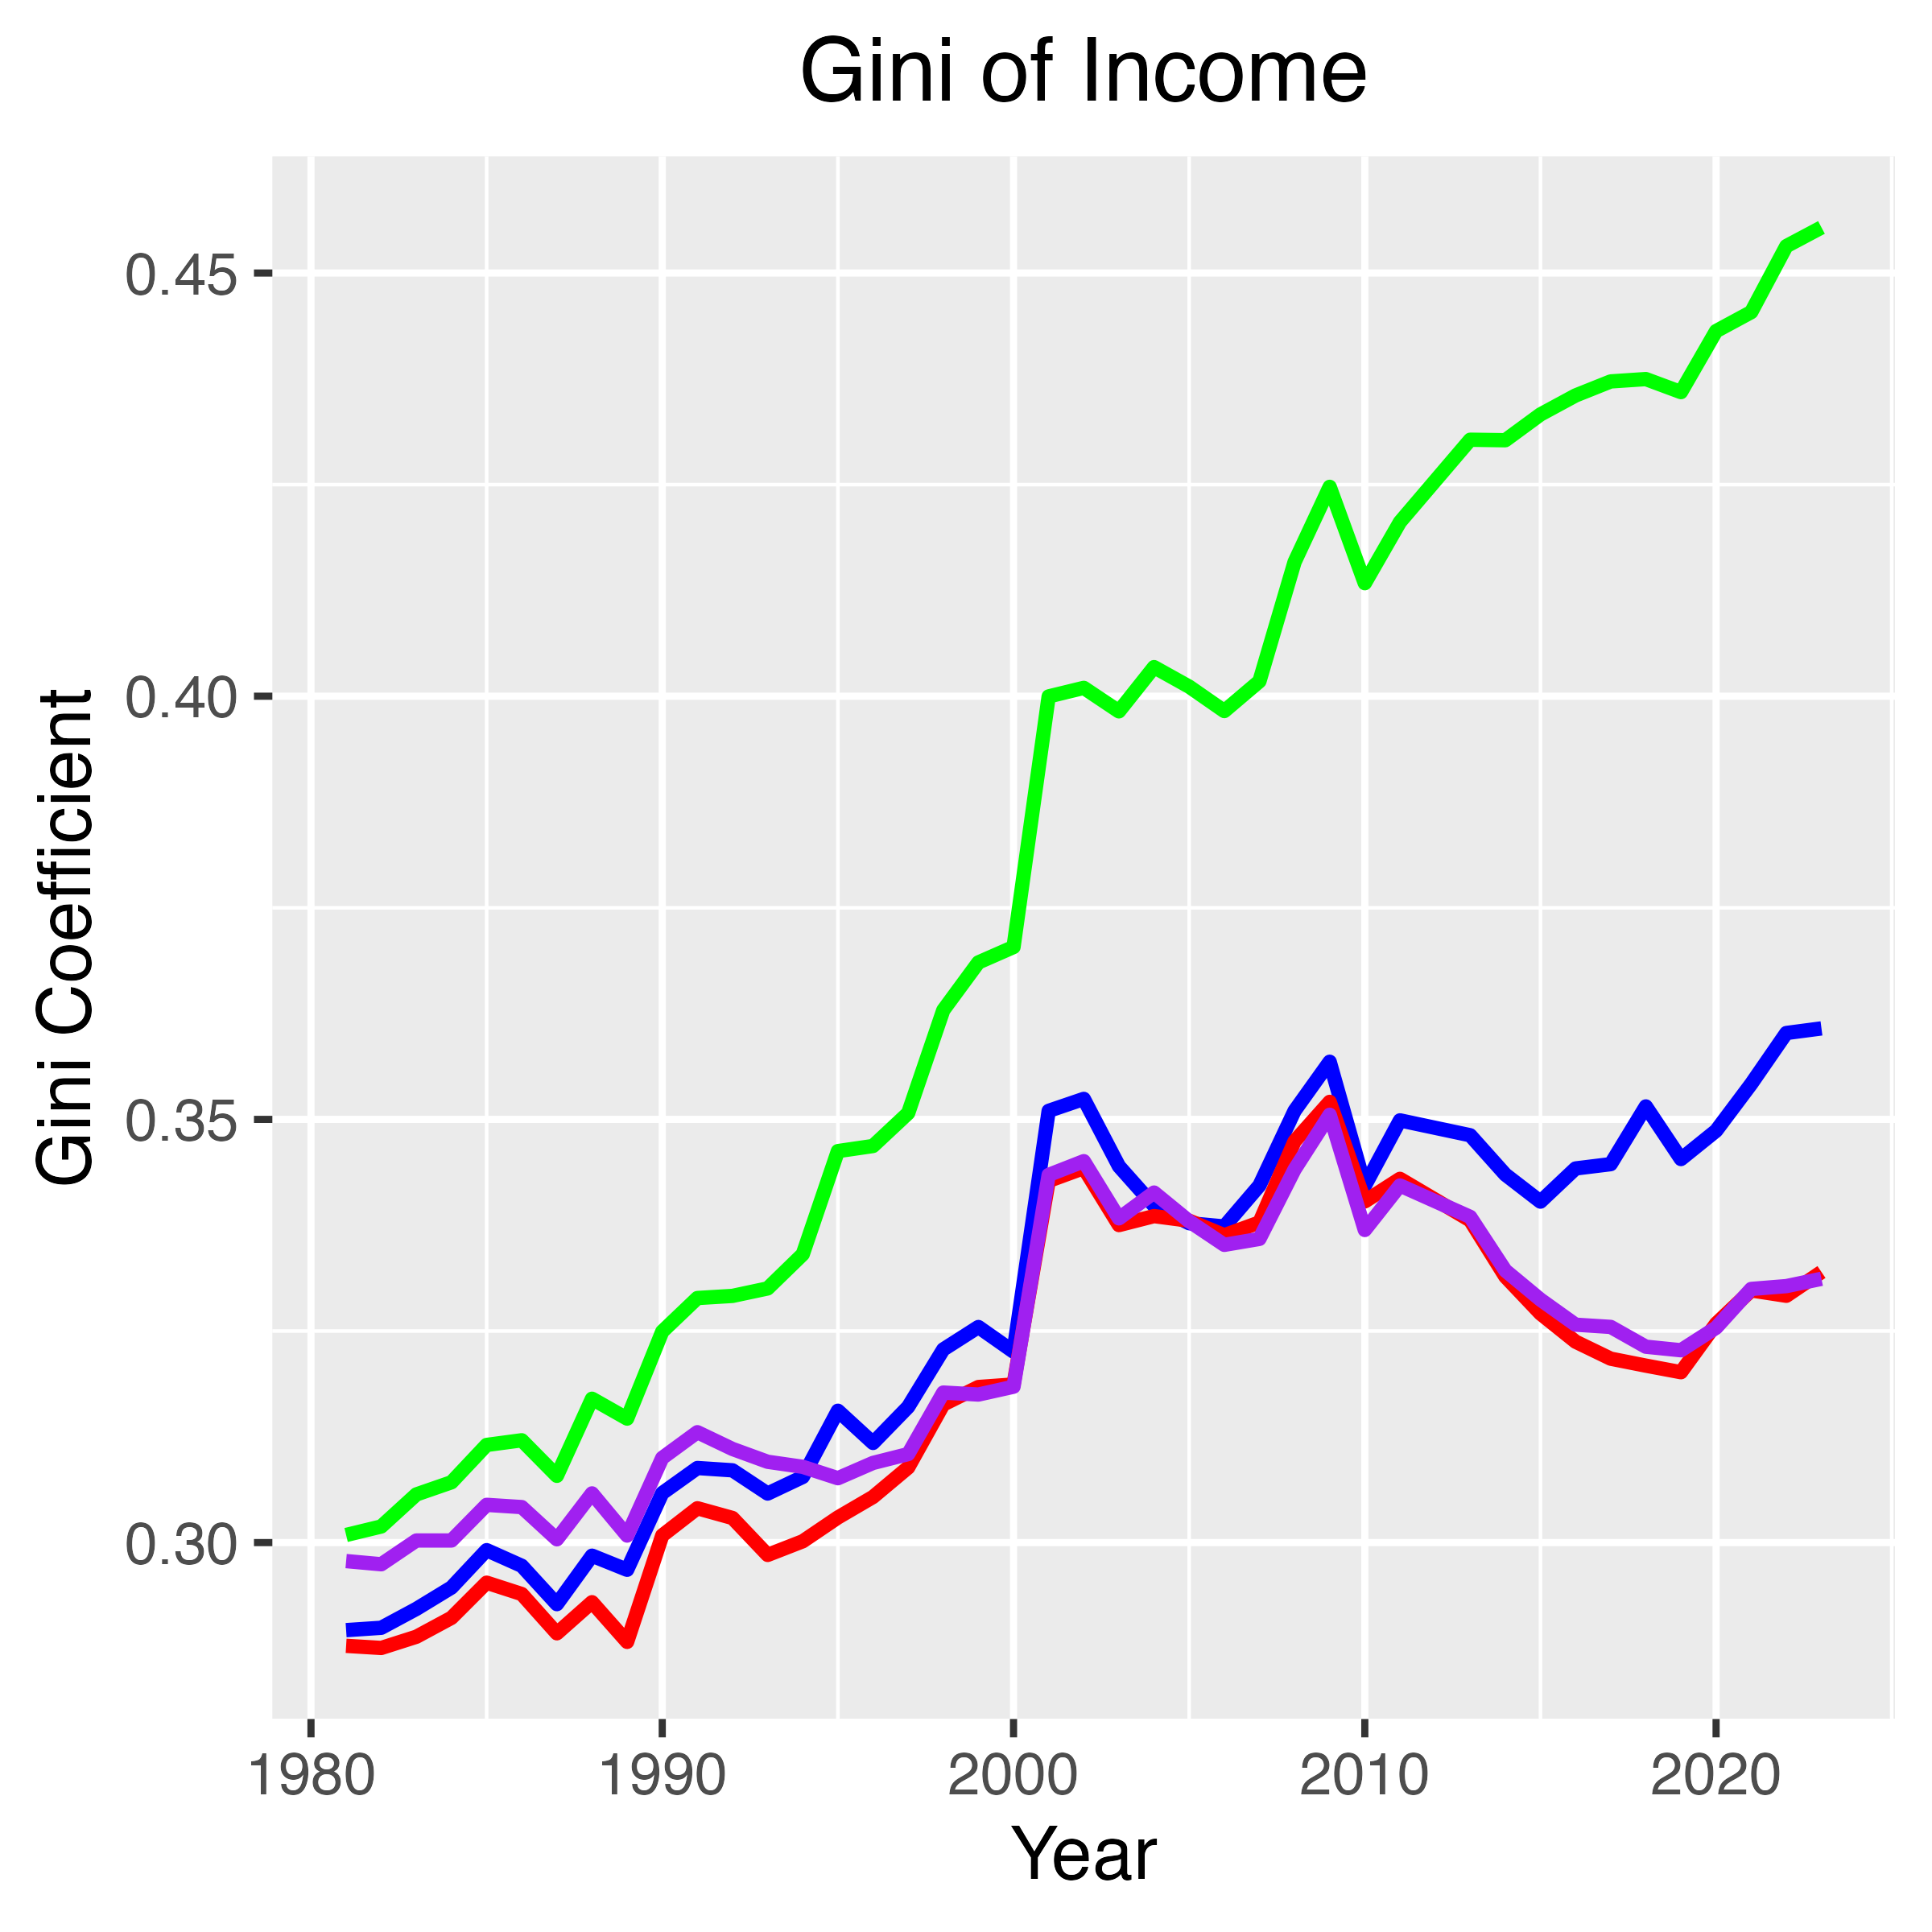
\includegraphics[width=\textwidth]{figures/Fig_4/Fig_4b_Gini_inc.png}
        \label{fig:Trans_Asset_Gini1}
    \end{subfigure}
    \begin{subfigure}[t]{0.475\textwidth}
        \centering
        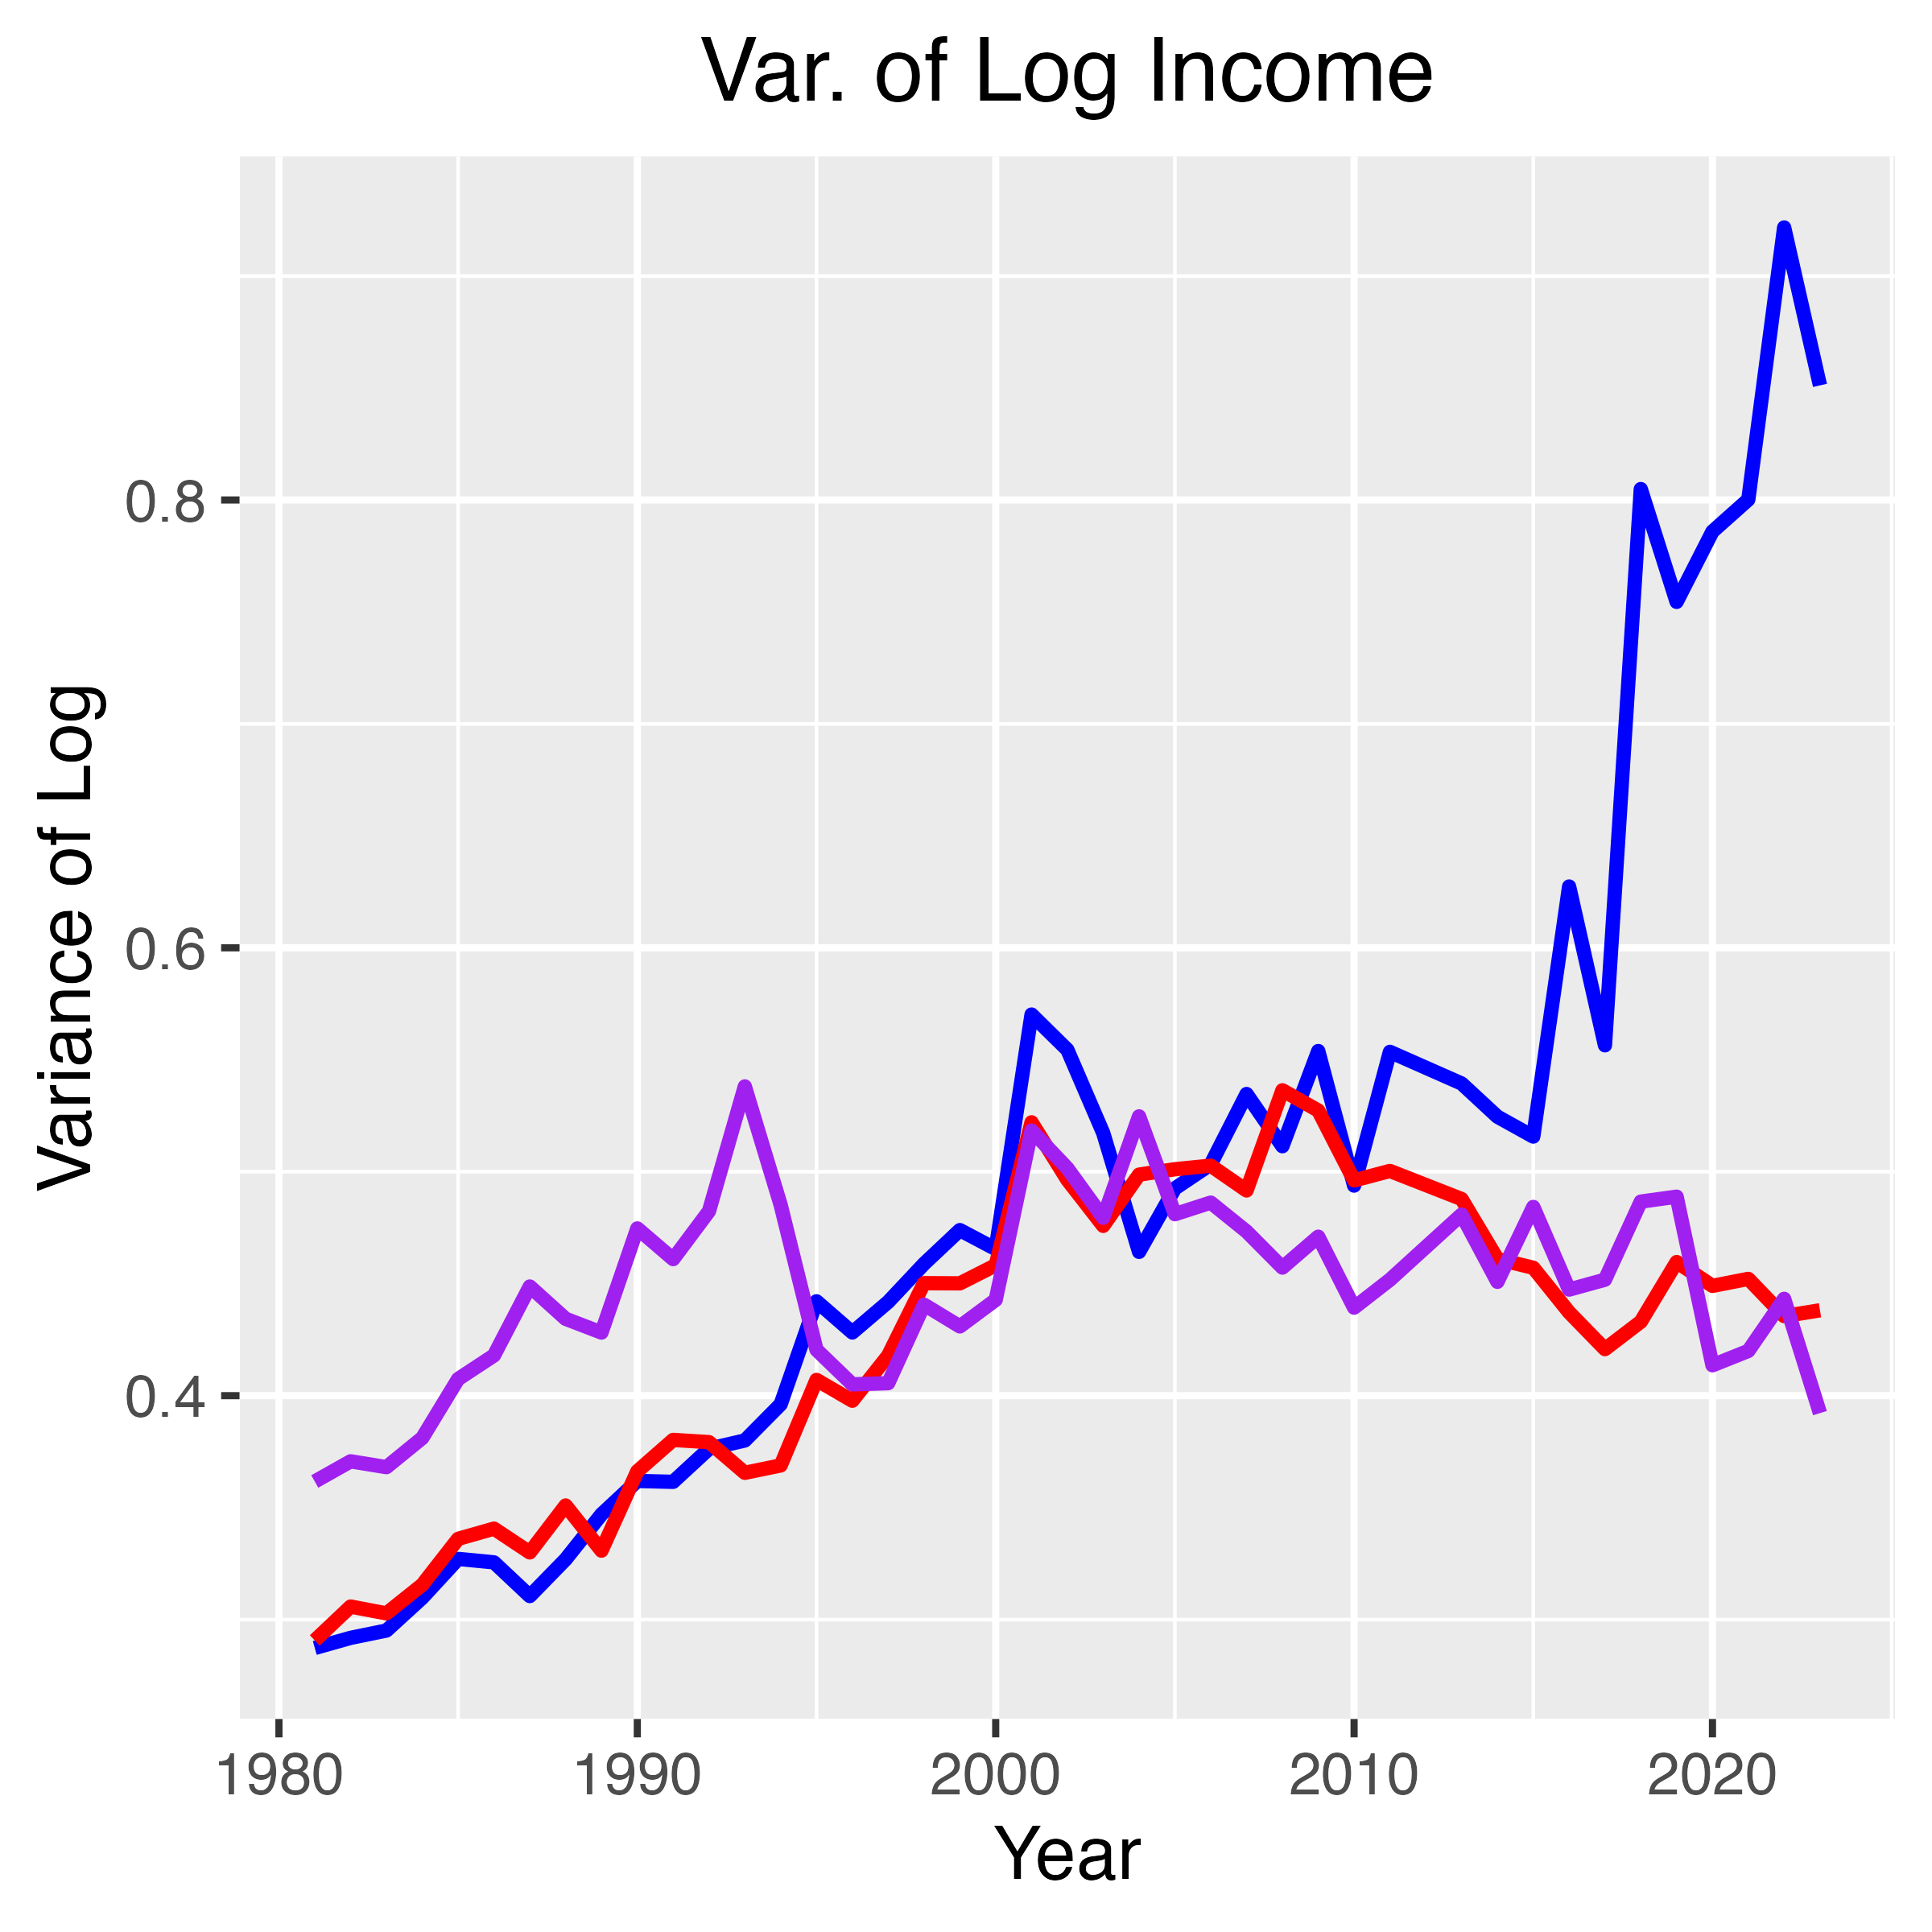
\includegraphics[width=\textwidth]{figures/Fig_4/Fig_4c_Var_inc.png}
        \label{fig:Trans_Asset_Var2}
    \end{subfigure}
    \begin{subfigure}[t]{0.475\textwidth}
        \centering
        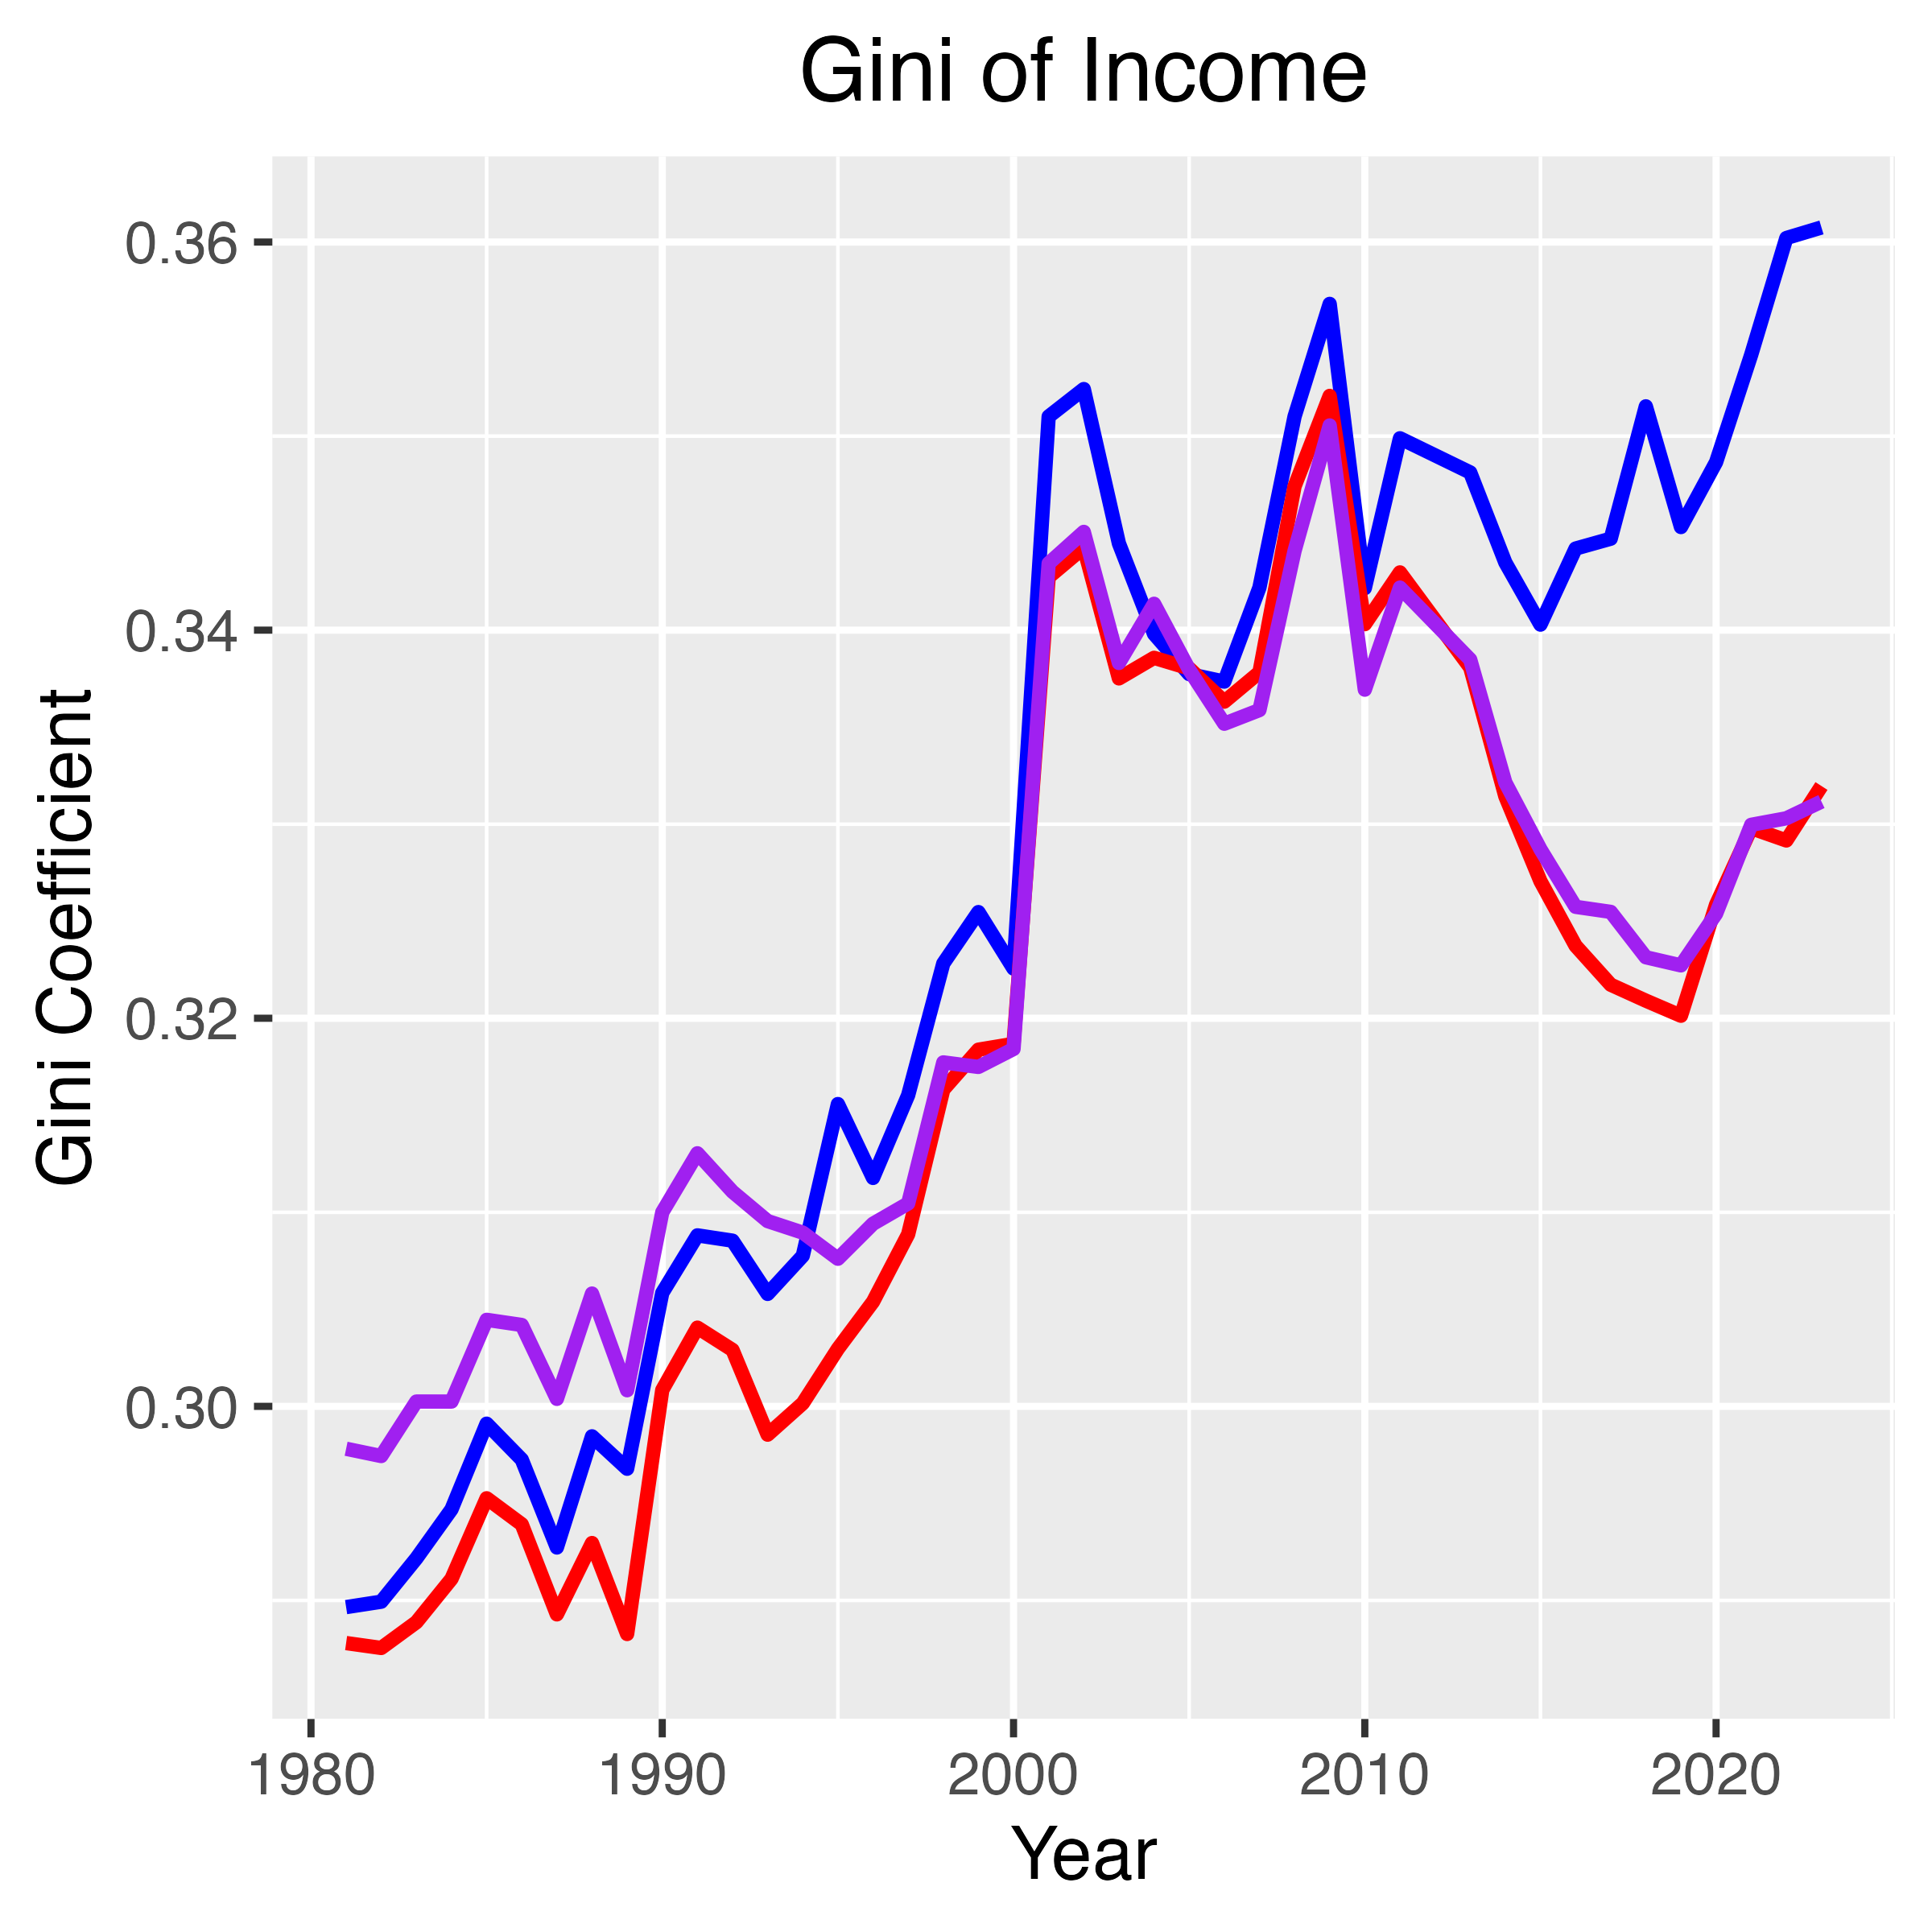
\includegraphics[width=\textwidth]{figures/Fig_4/Fig_4d_Gini_inc.png}
        \label{fig:Trans_Asset_Gini2}
    \end{subfigure}
    \caption{From Household Earnings to Pre-Government Income}
    \label{fig:Trans_Asset}
\end{figure}

\subsection{Government Redistribution}

\begin{figure}
    \centering
    \begin{subfigure}[t]{0.475\textwidth}
        \centering
        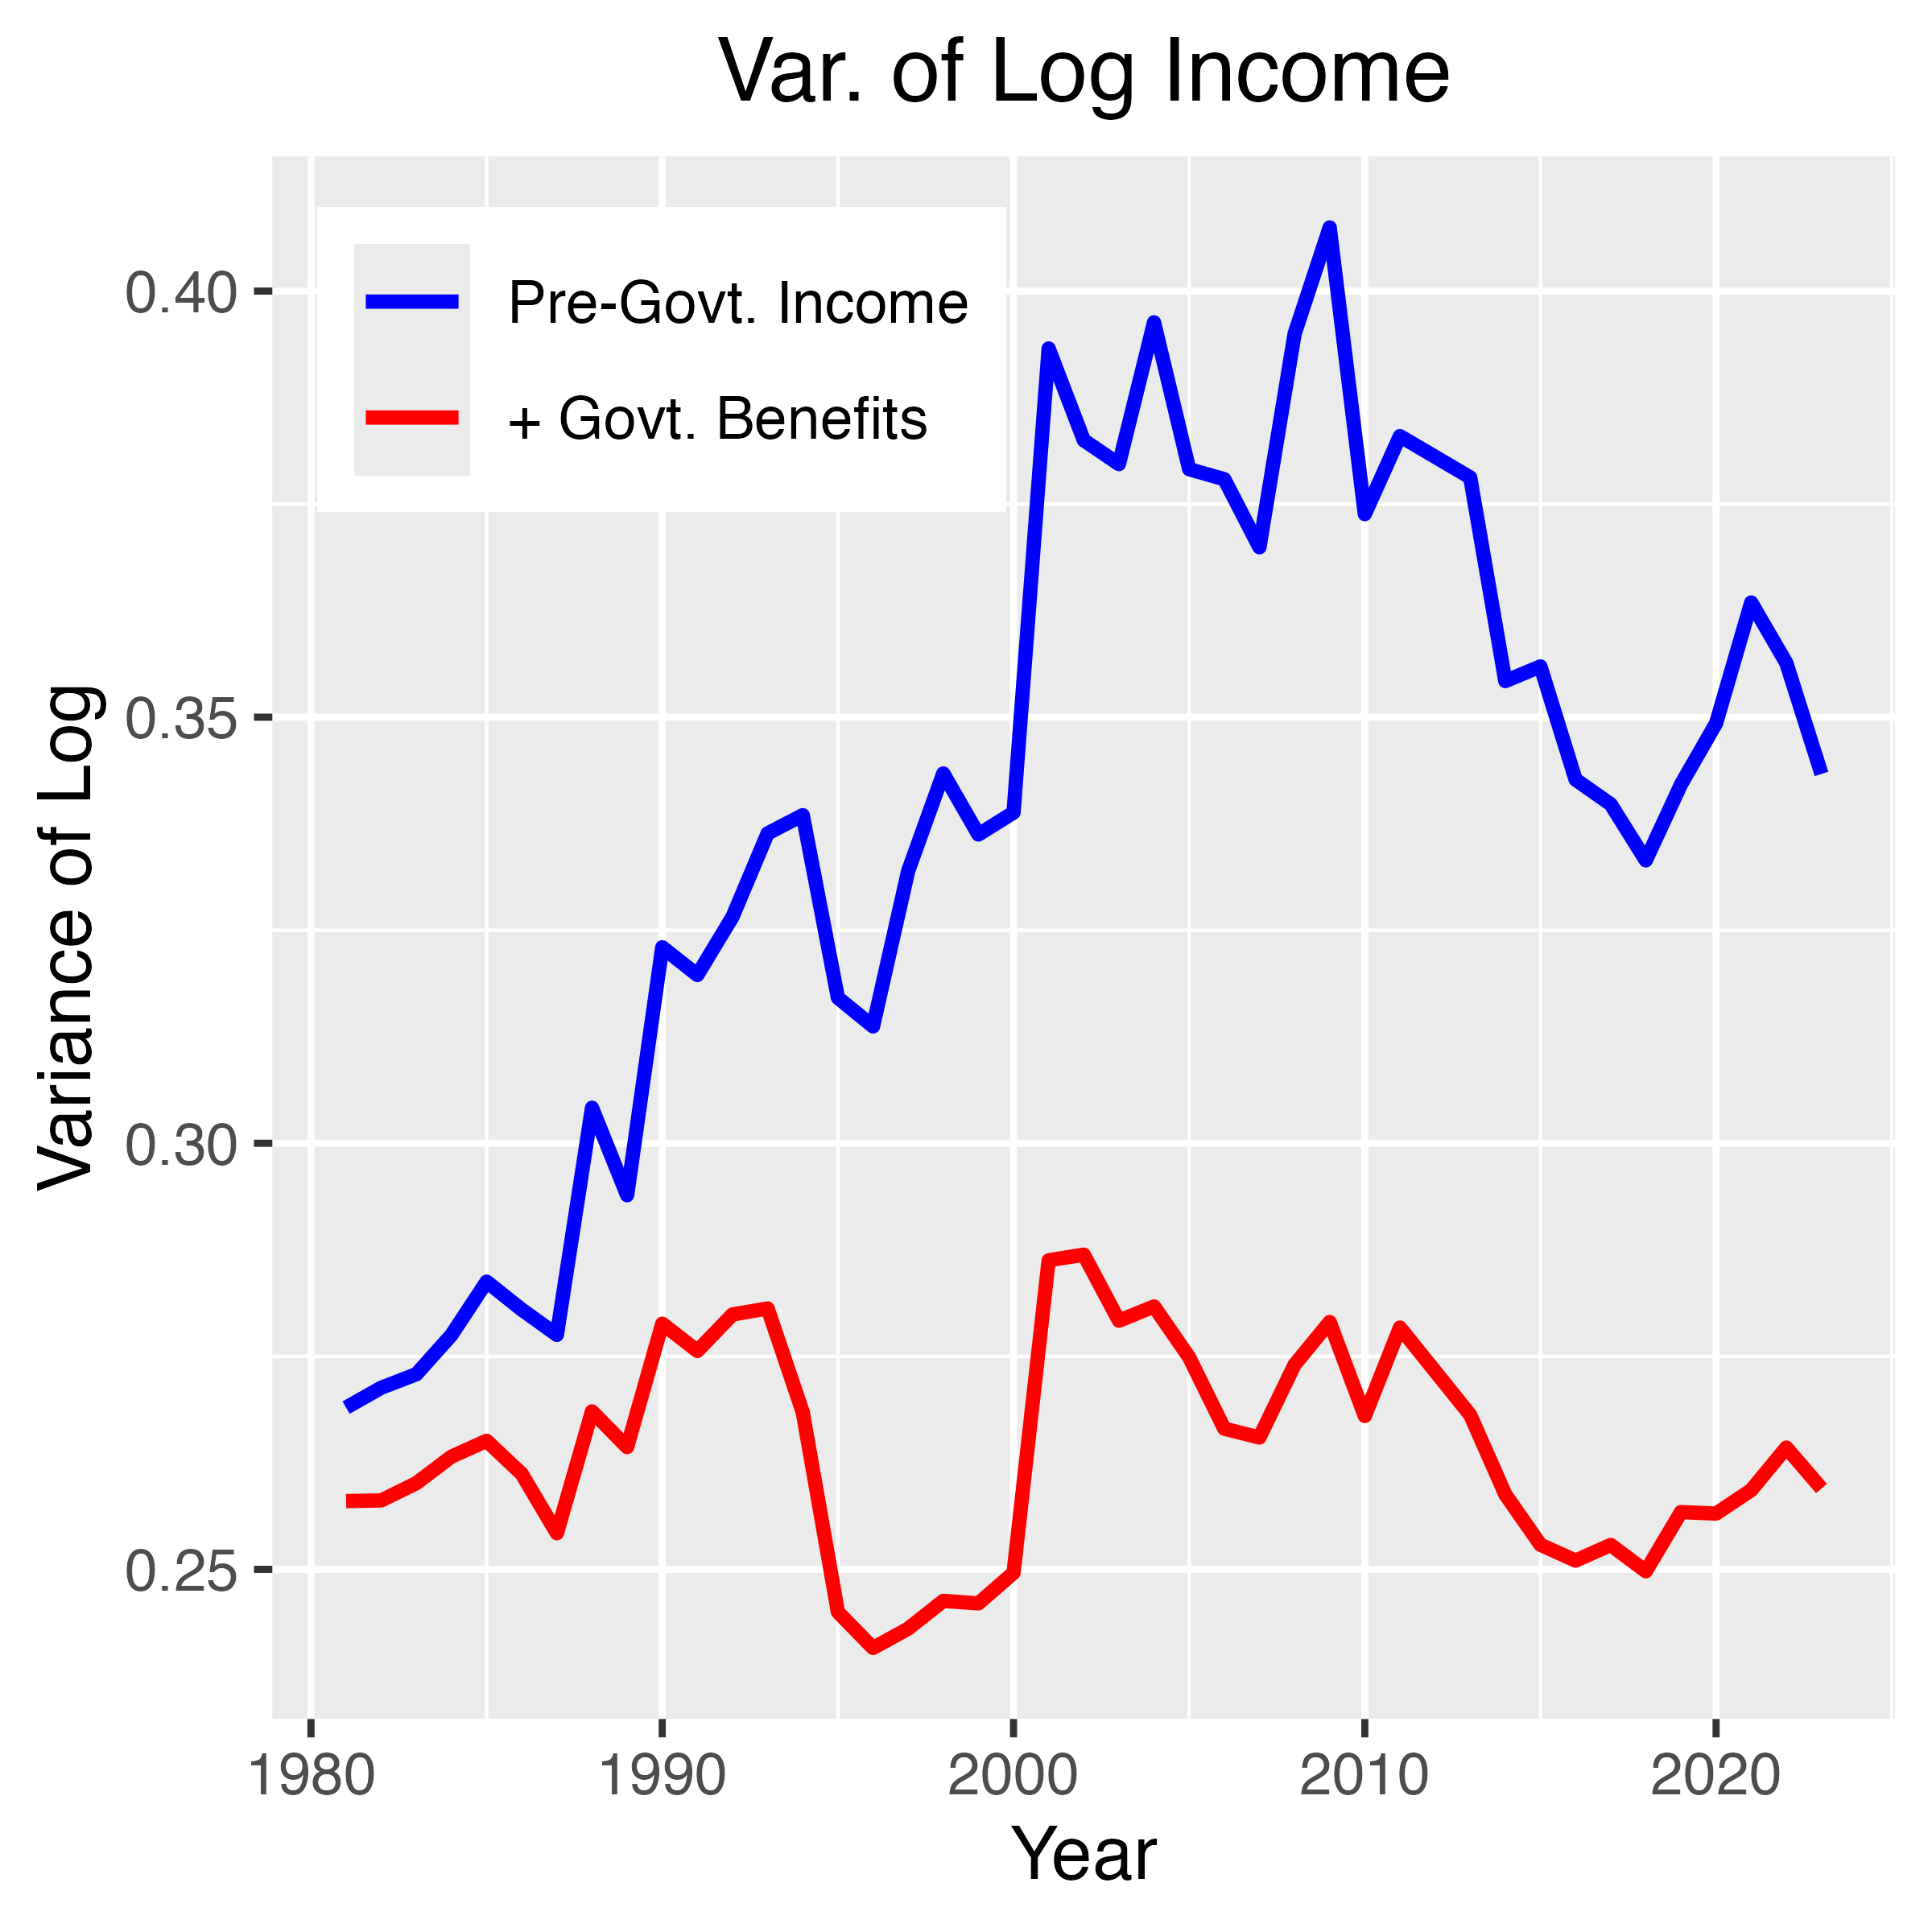
\includegraphics[width=\textwidth]{figures/Fig_5/Fig_5a_Var_inc.png}
        \label{fig:Gov_Var1}
    \end{subfigure}
    \begin{subfigure}[t]{0.475\textwidth}
        \centering
        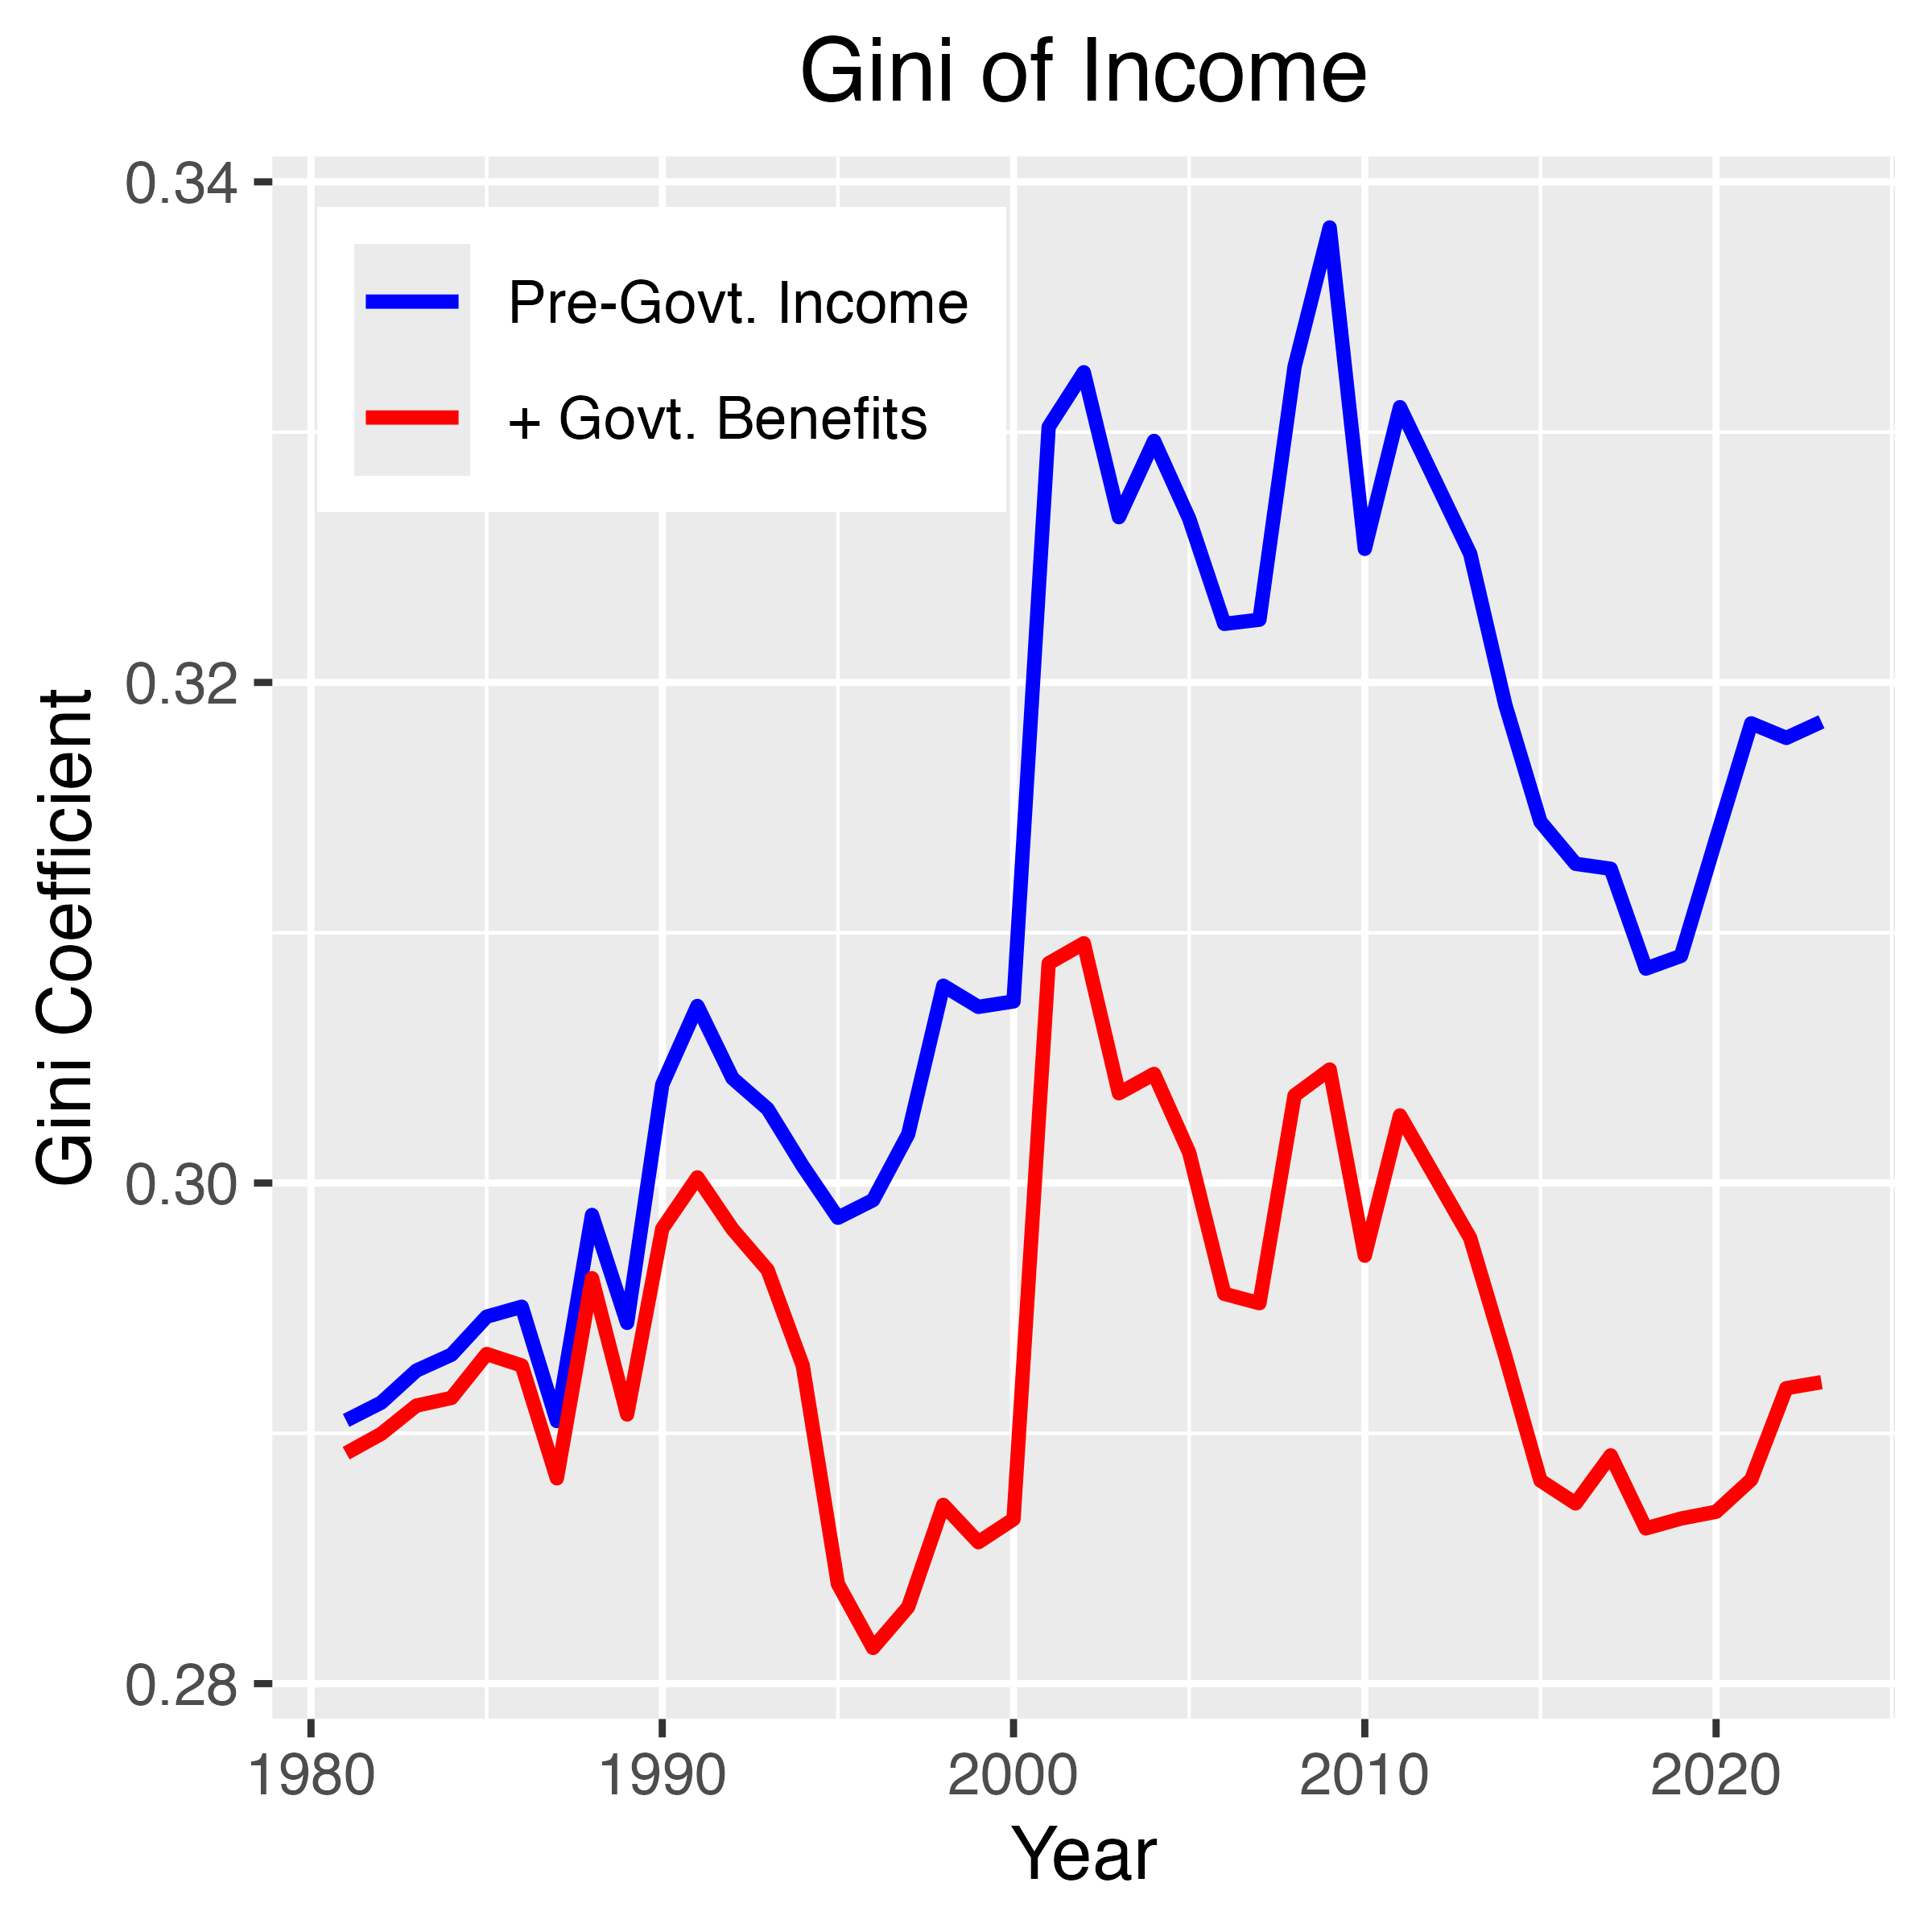
\includegraphics[width=\textwidth]{figures/Fig_5/Fig_5b_Gini_inc.png}
        \label{fig:Gov_Gini1}
    \end{subfigure}
    \begin{subfigure}[t]{0.475\textwidth}
        \centering
        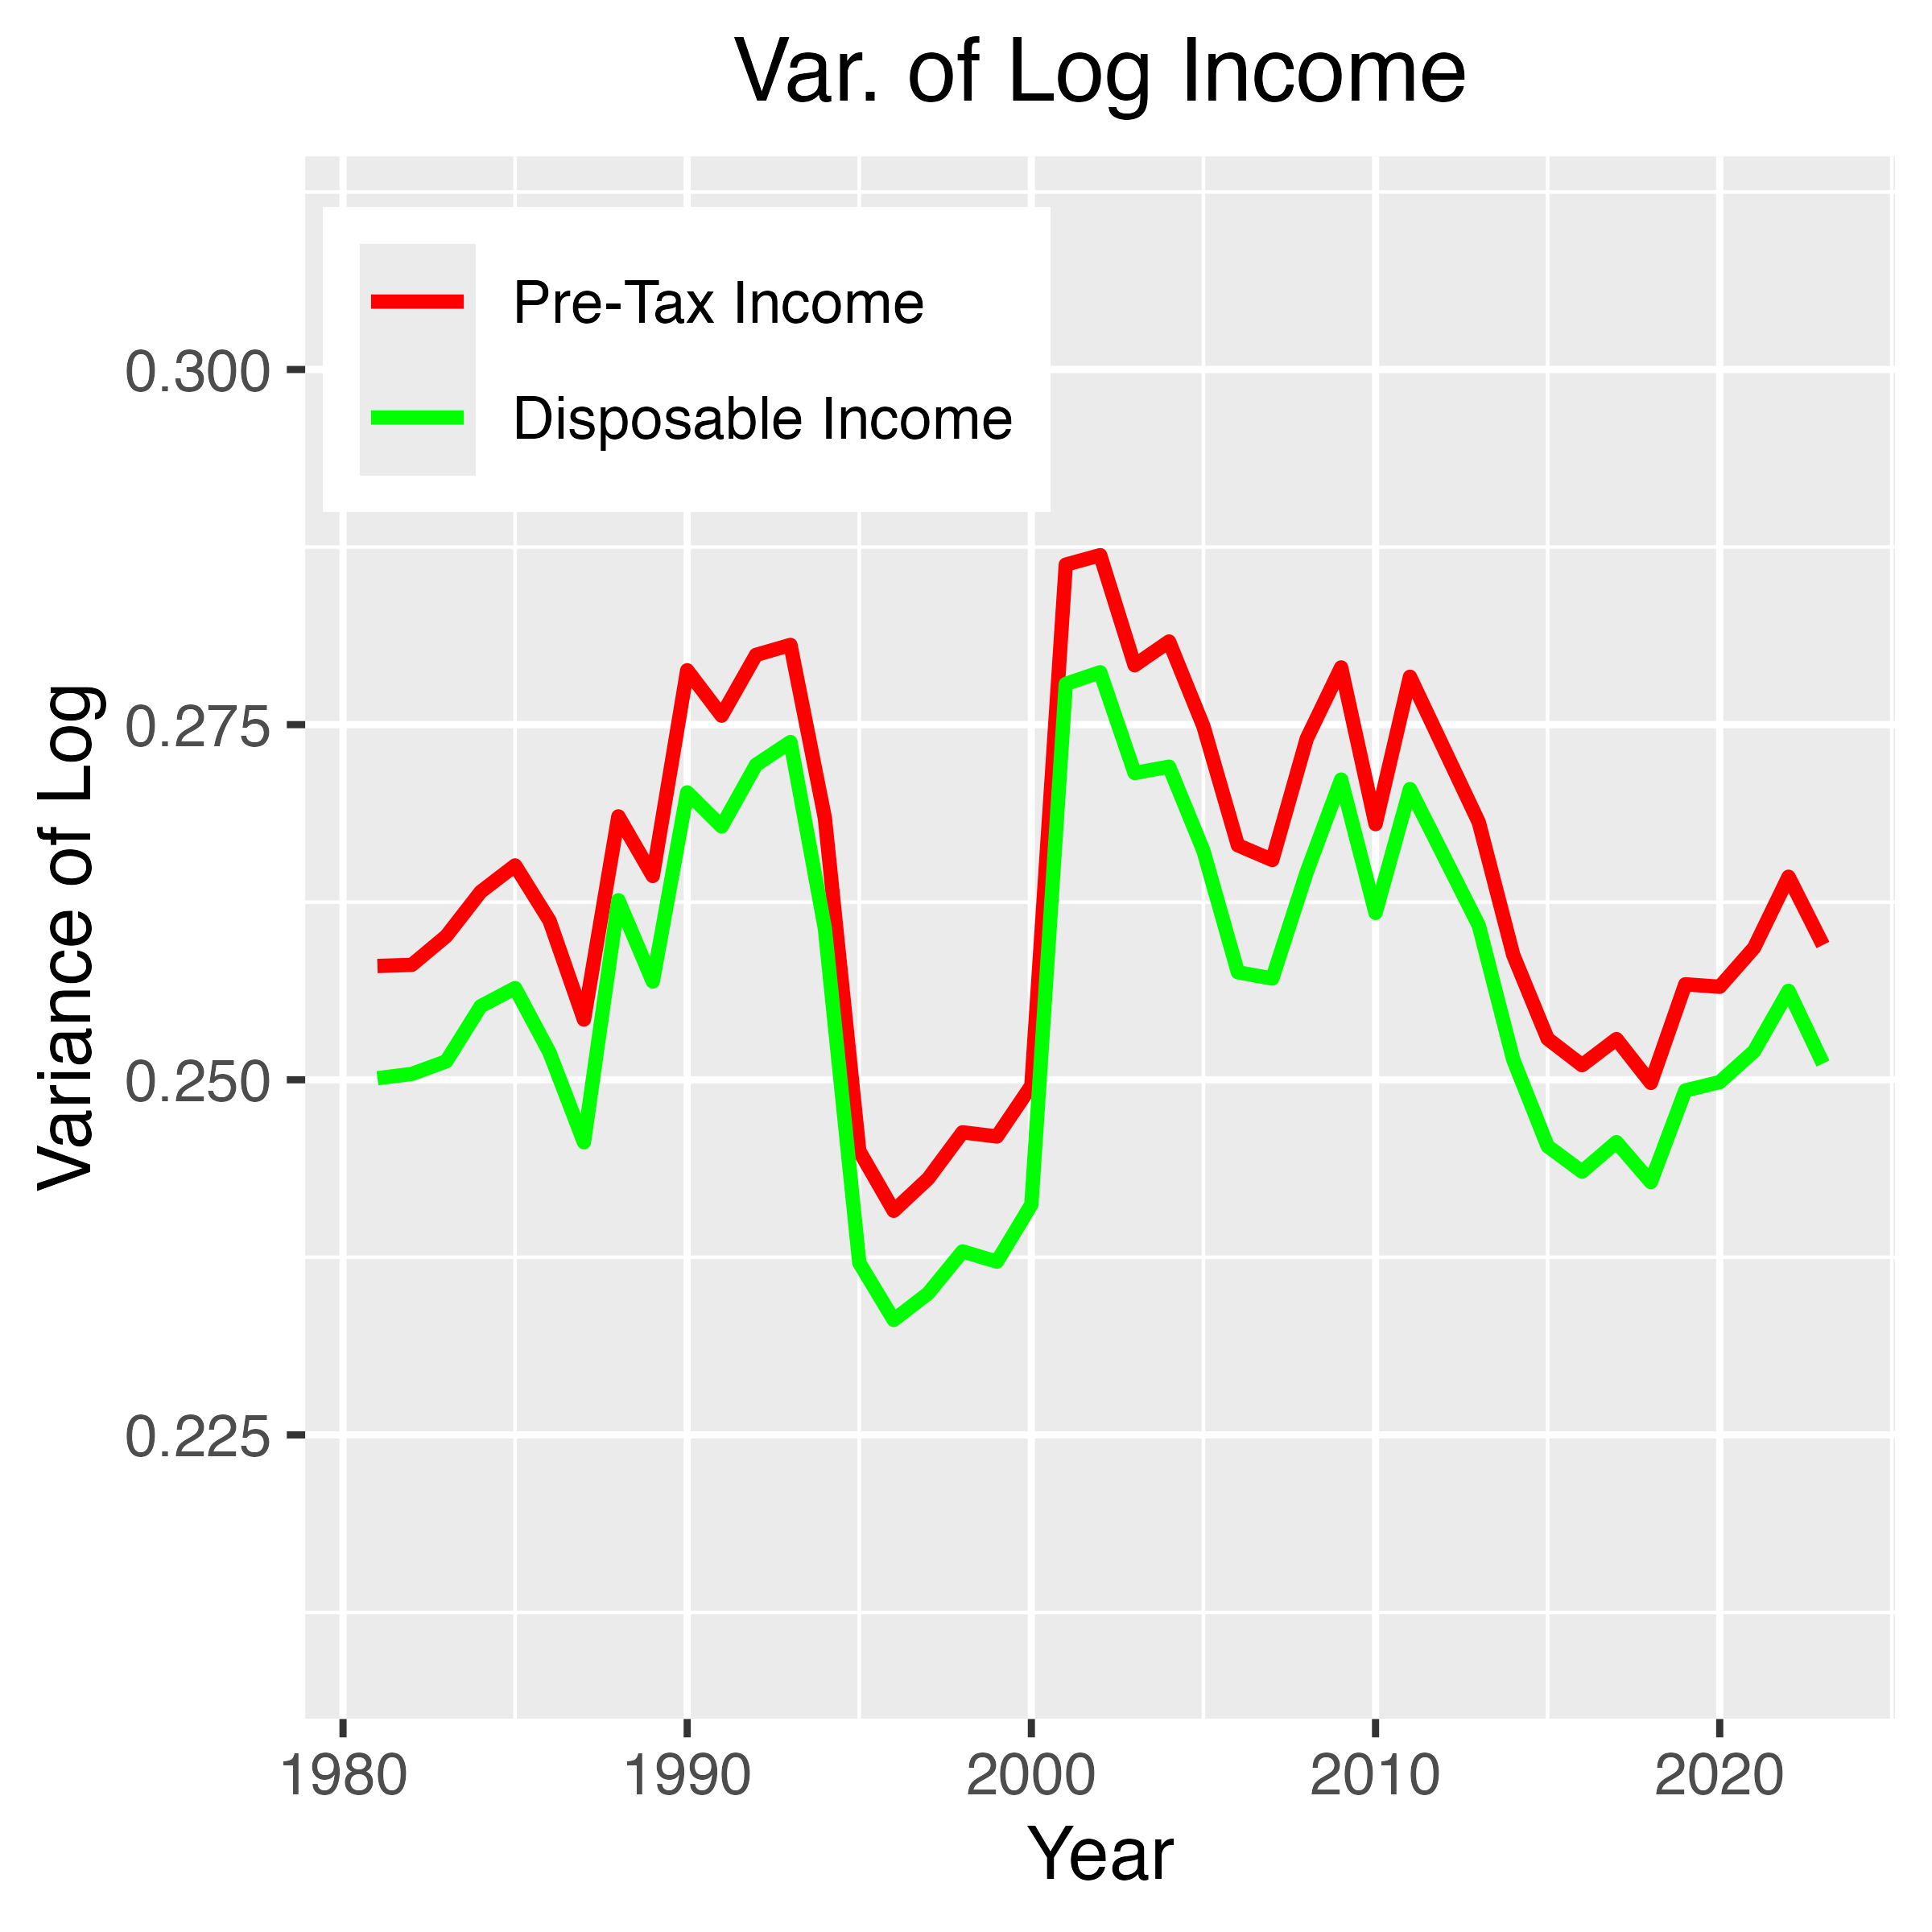
\includegraphics[width=\textwidth]{figures/Fig_5/Fig_5c_Var_inc.png}
        \label{fig:Gov_Var2}
    \end{subfigure}
    \begin{subfigure}[t]{0.475\textwidth}
        \centering
        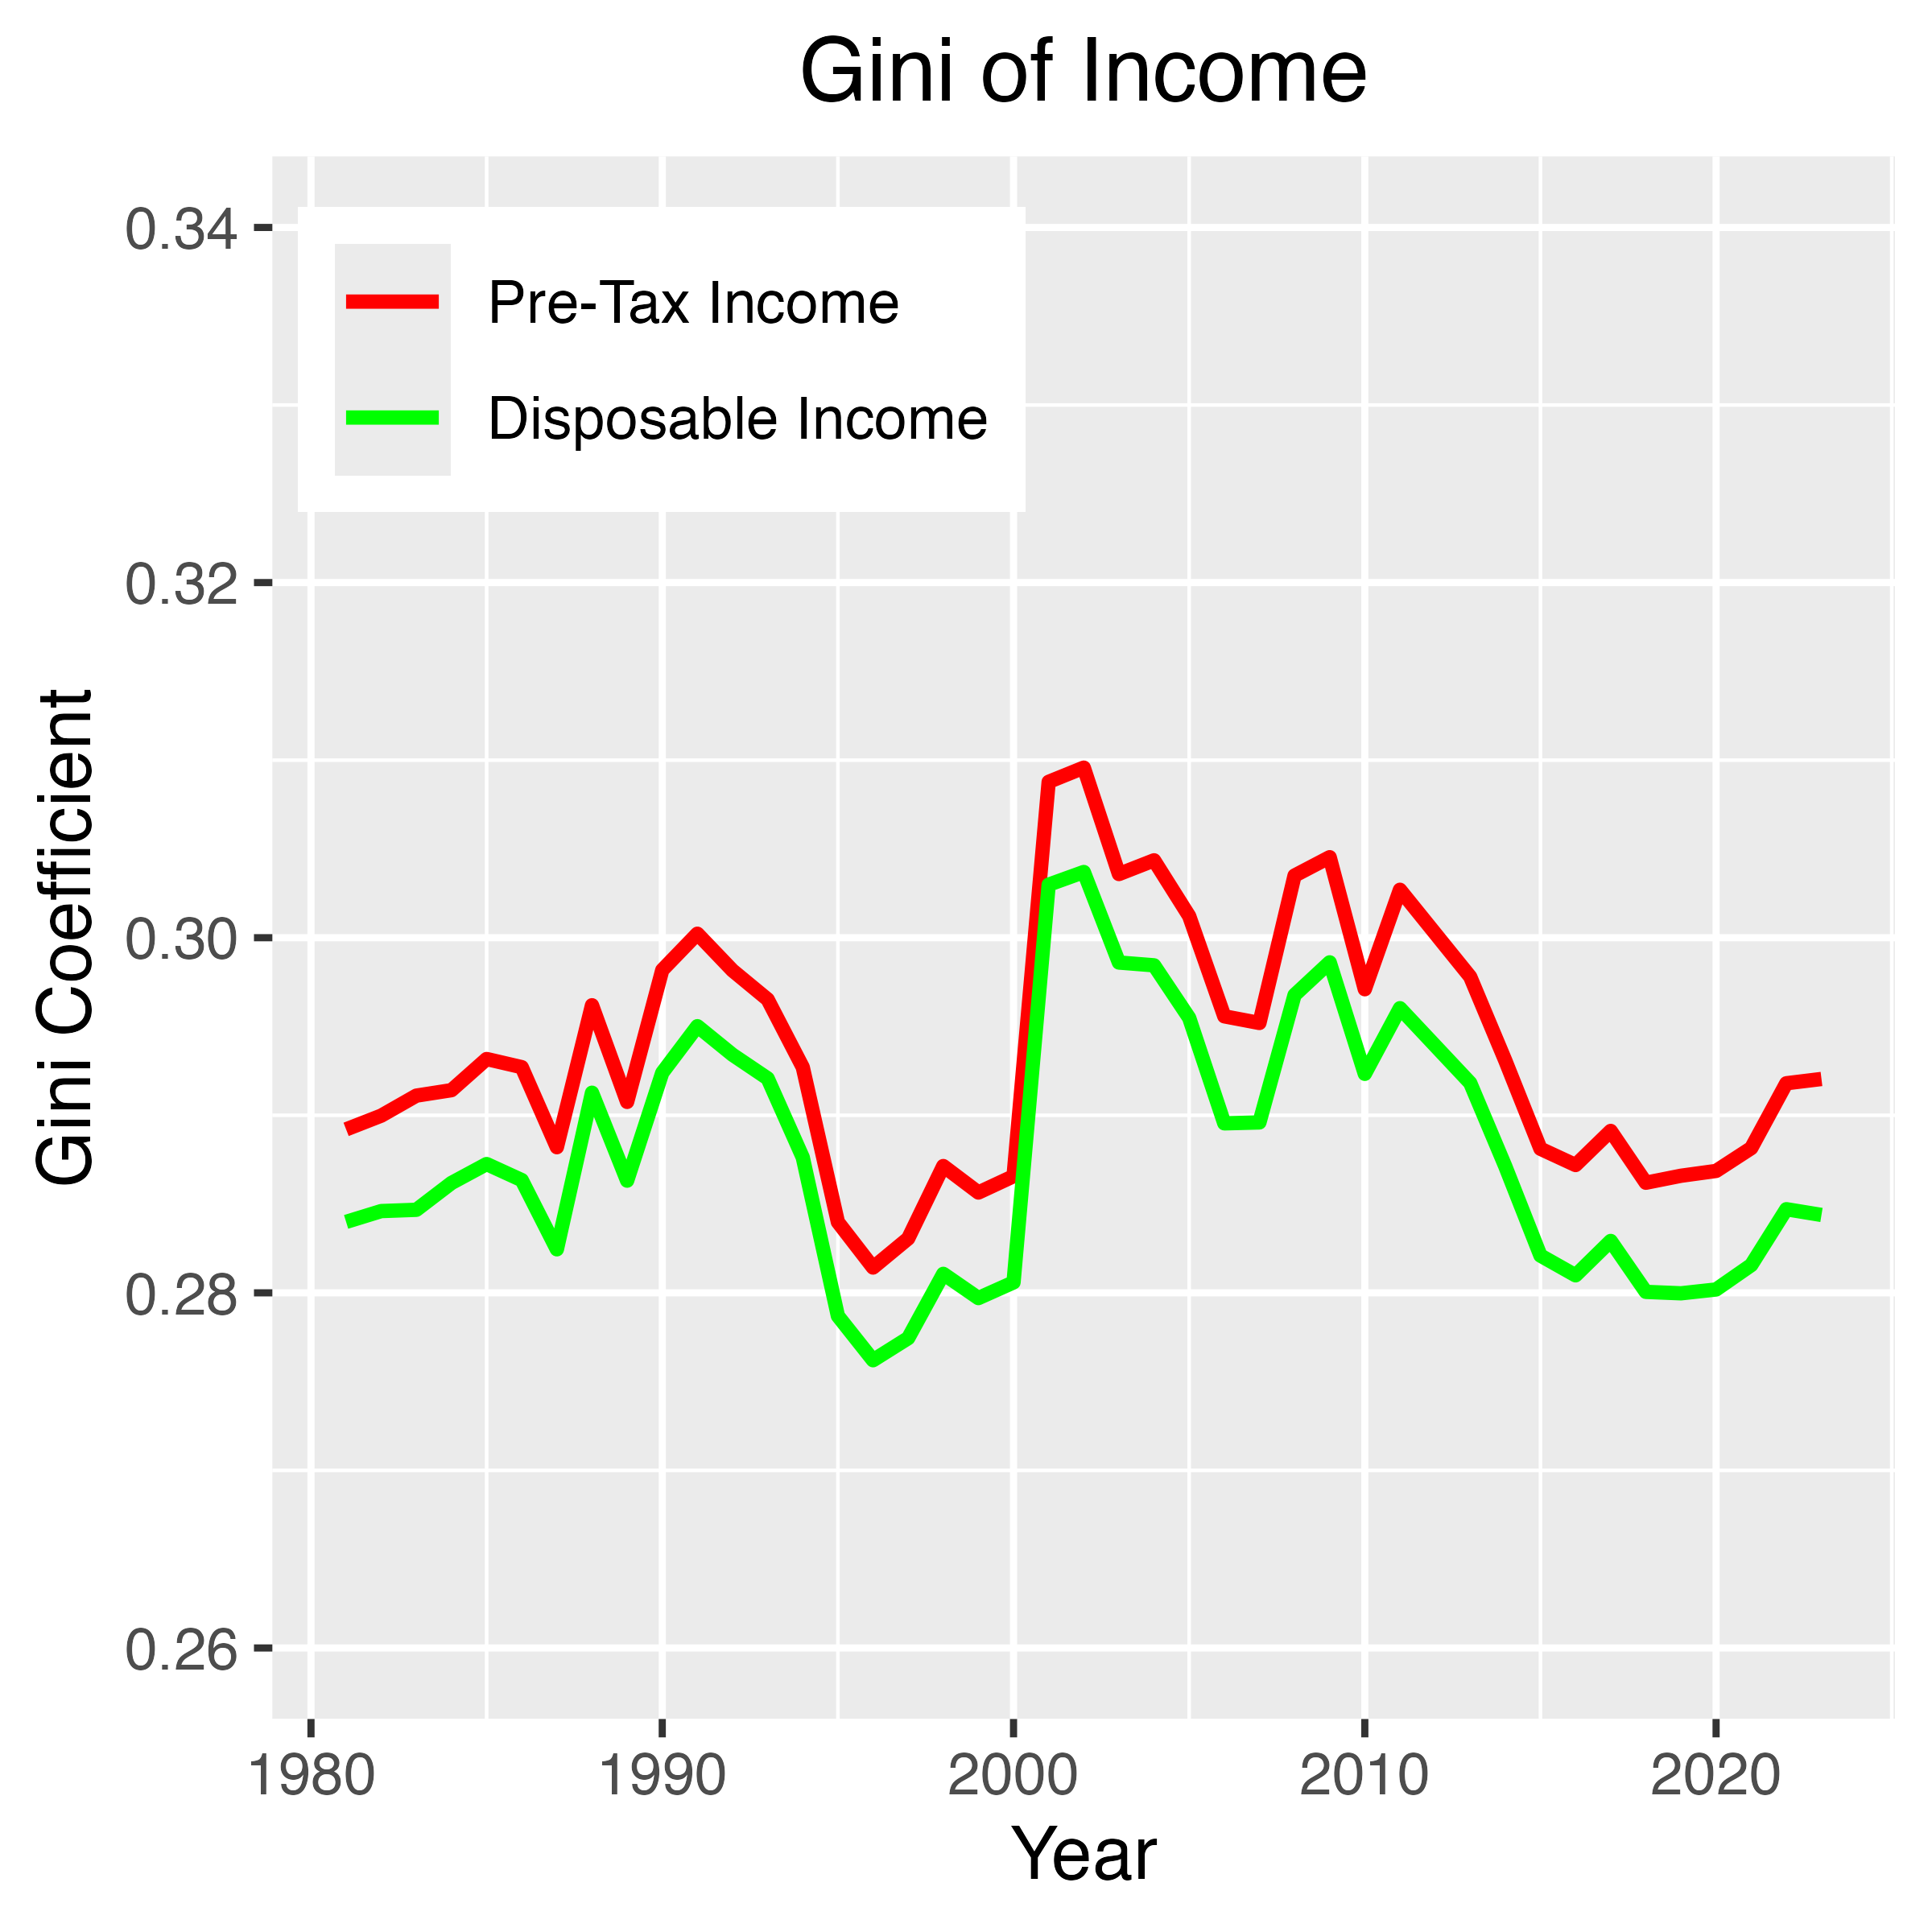
\includegraphics[width=\textwidth]{figures/Fig_5/Fig_5d_Gini_inc.png}
        \label{fig:Gov_Gini2}
    \end{subfigure}
    \caption{From Pre-Government to Disposable Income}
    \label{fig:Gov}
\end{figure}

\subsection{From Income to Consumption Inequality}

\begin{figure}
    \centering
    \begin{subfigure}[t]{0.475\textwidth}
        \centering
        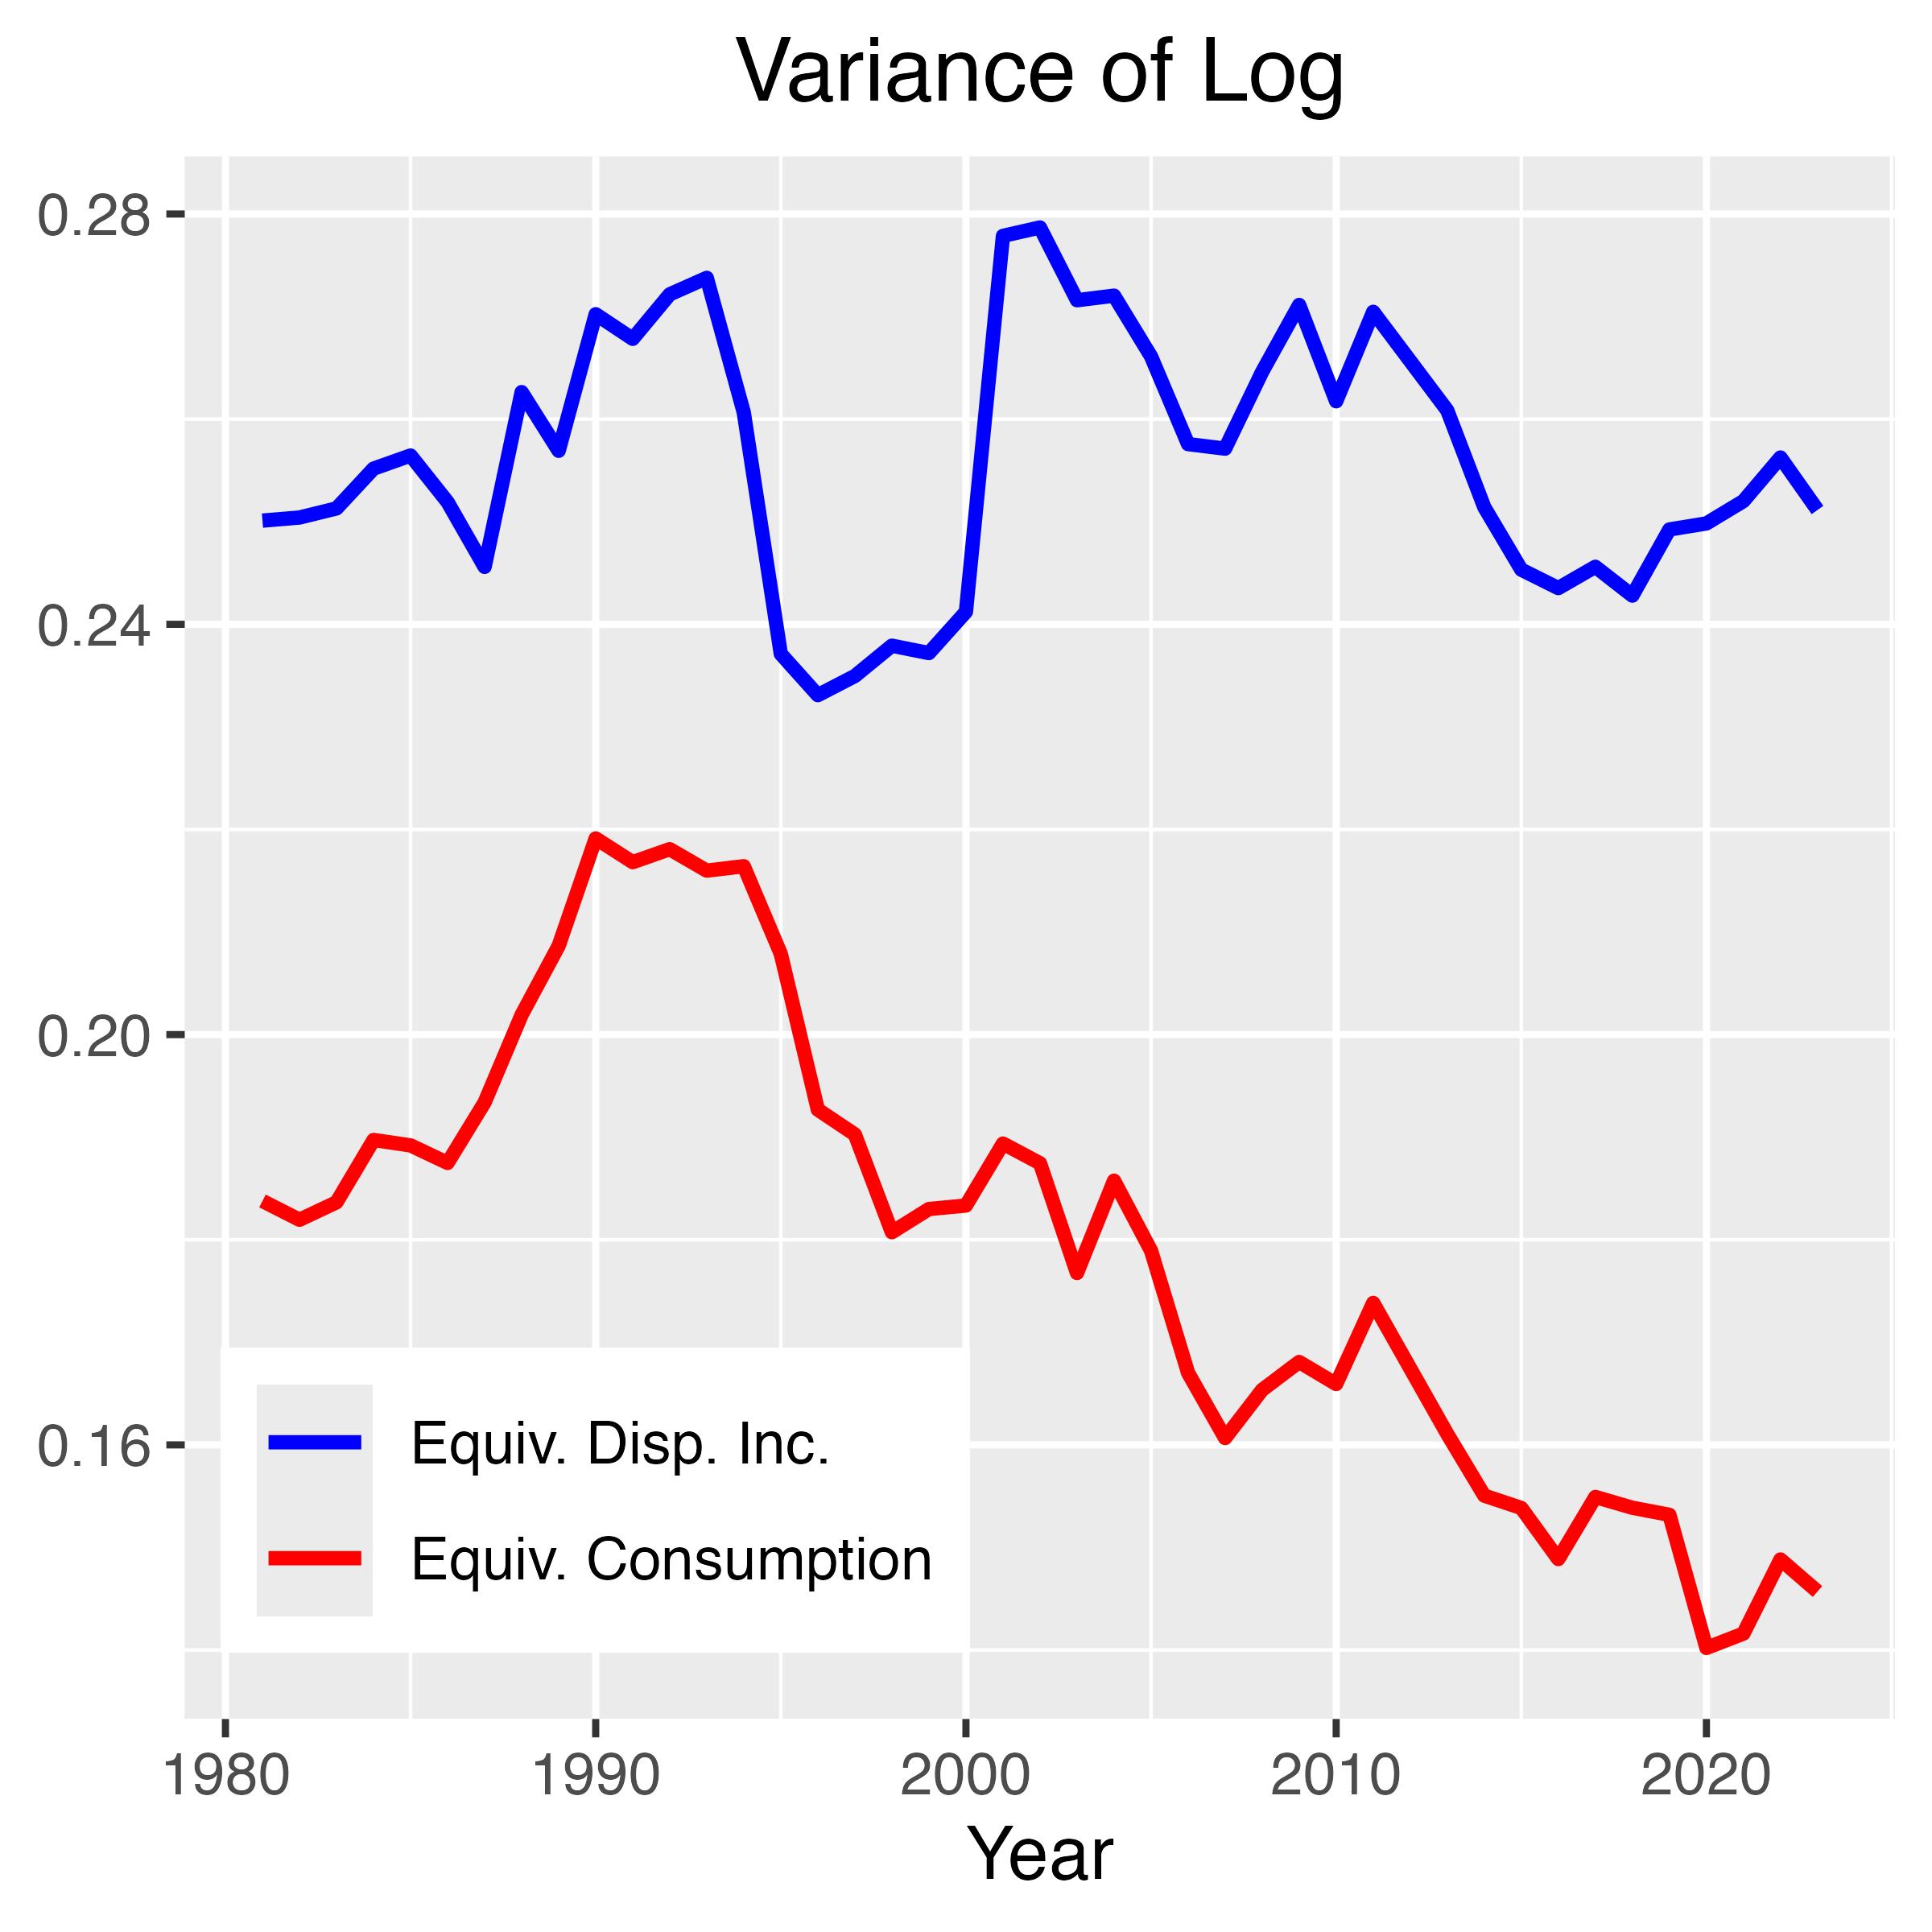
\includegraphics[width=\textwidth]{figures/Fig_6/Fig_6a.png}
        \label{fig:Consumption_Var}
    \end{subfigure}
    \begin{subfigure}[t]{0.475\textwidth}
        \centering
        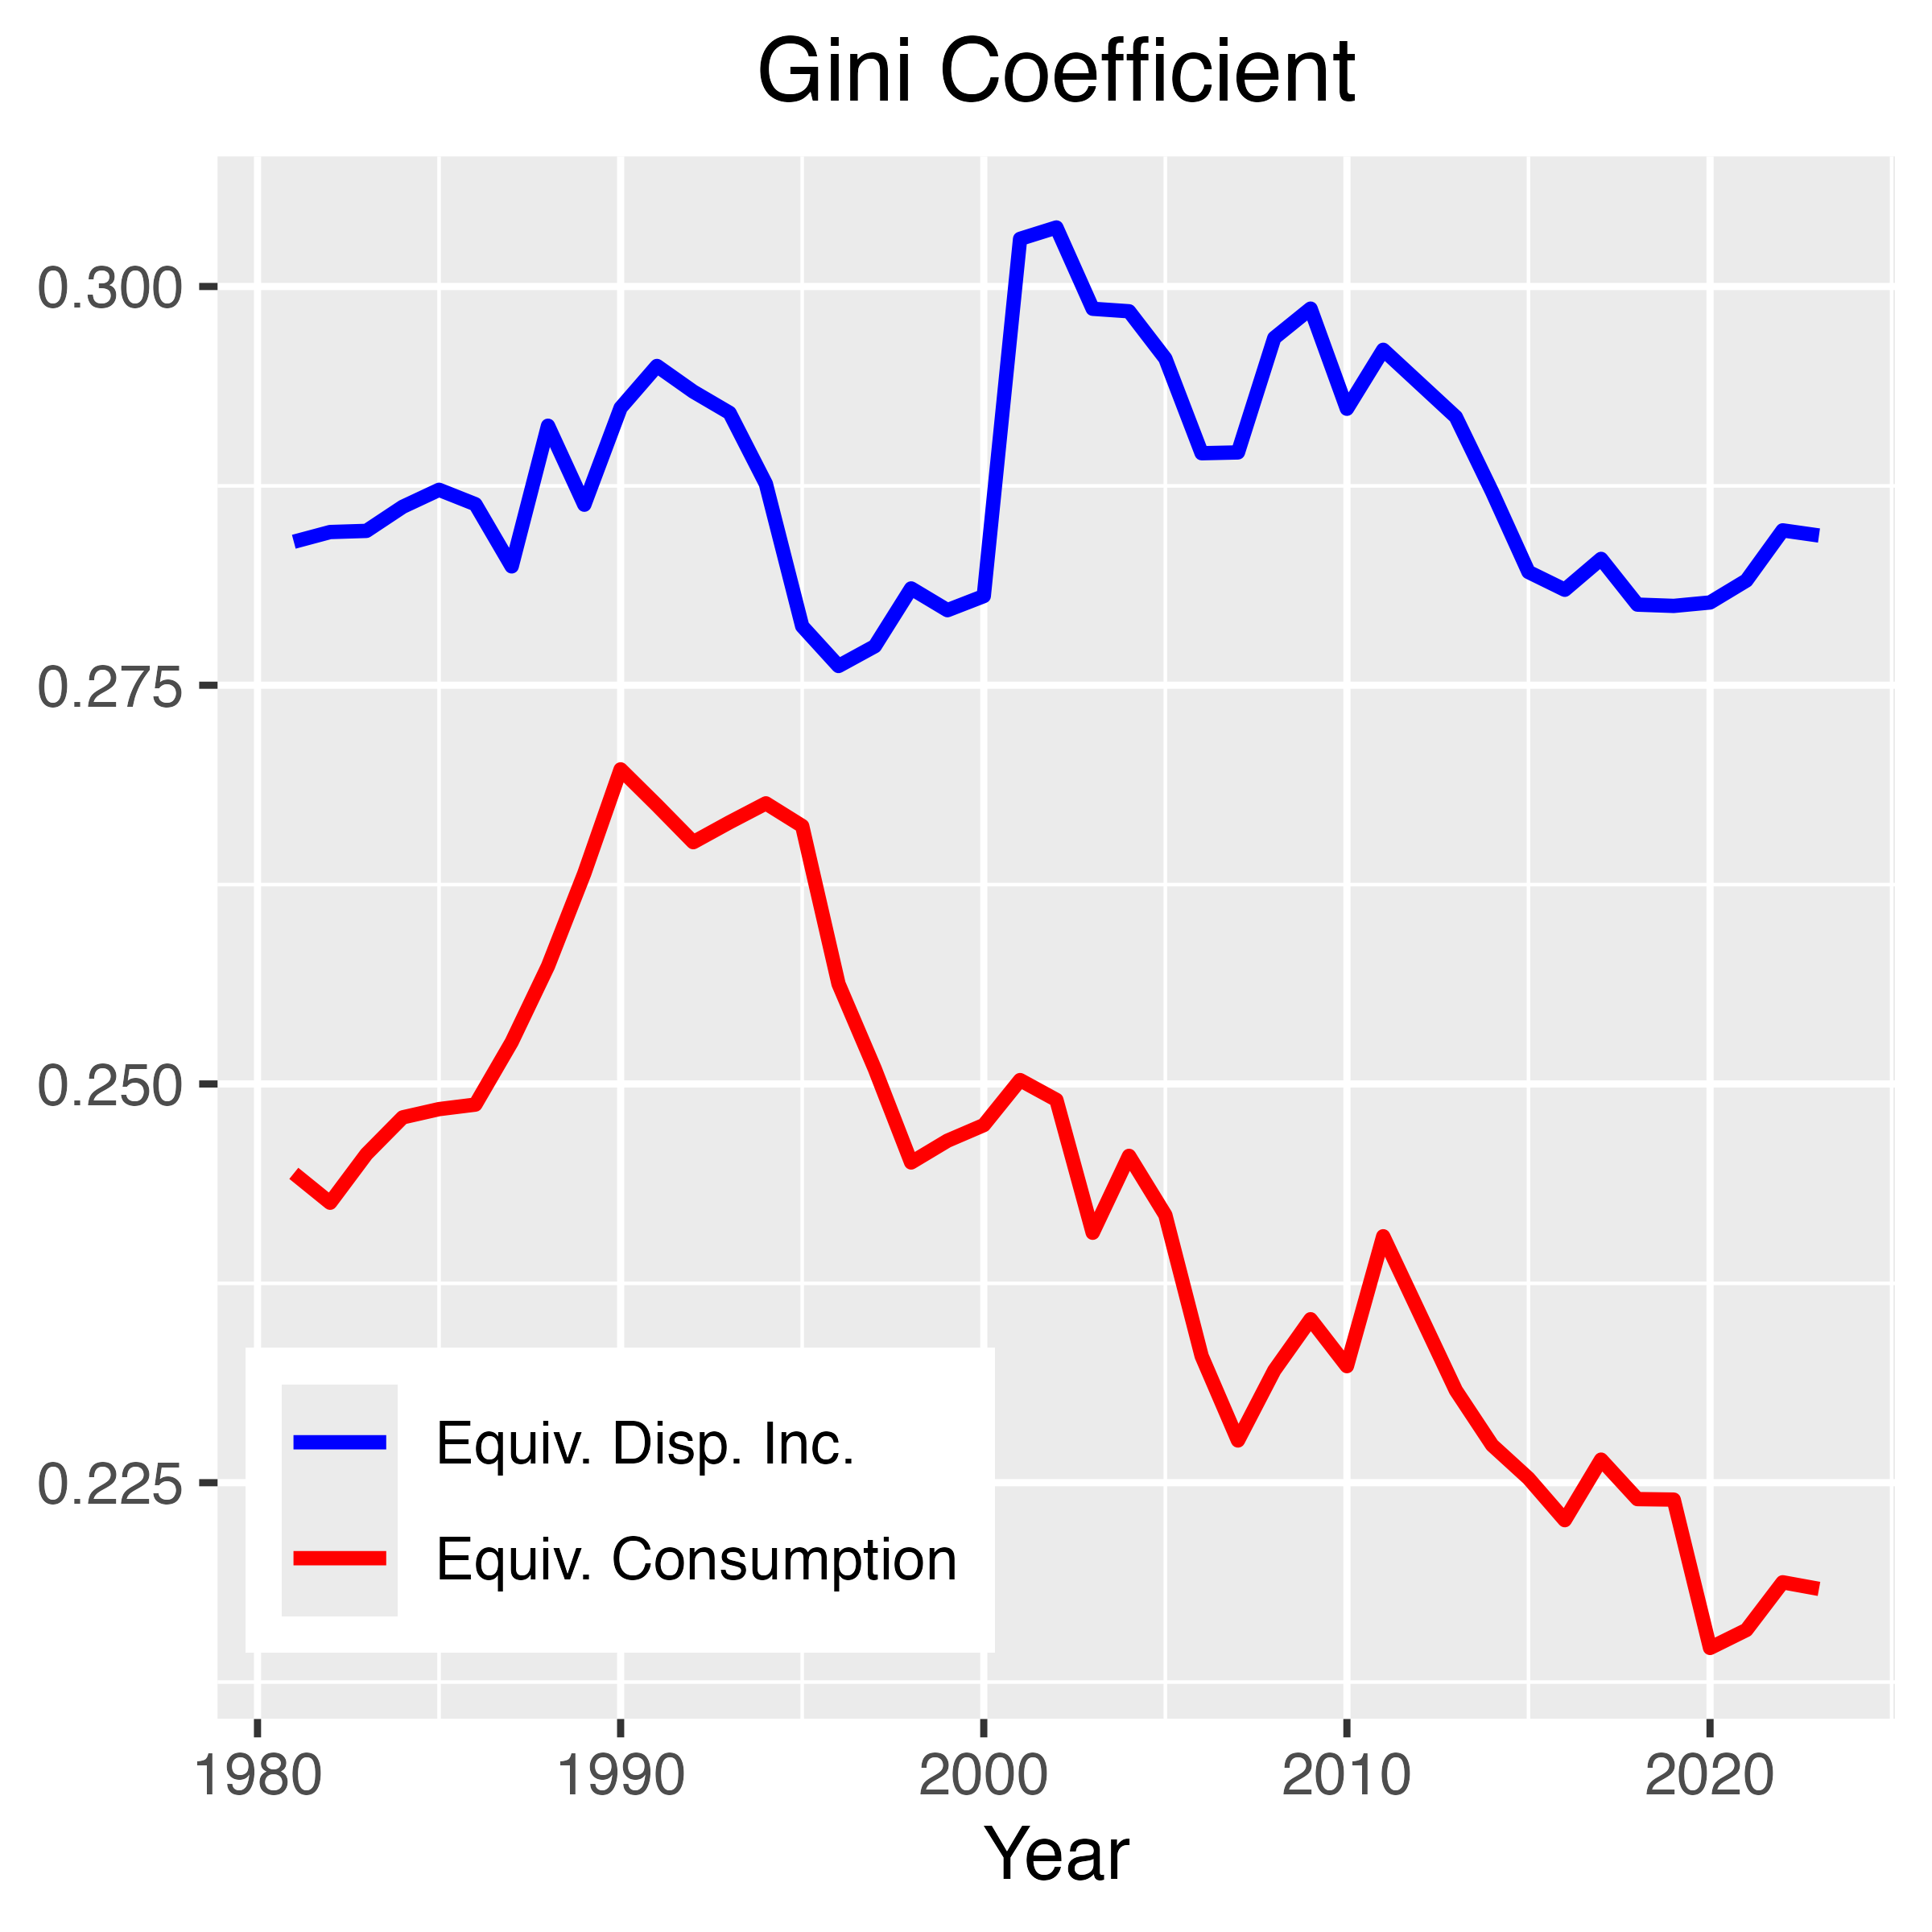
\includegraphics[width=\textwidth]{figures/Fig_6/Fig_6b.png}
        \label{fig:Consumption_Gini}
    \end{subfigure}
    \begin{subfigure}[t]{0.475\textwidth}
        \centering
        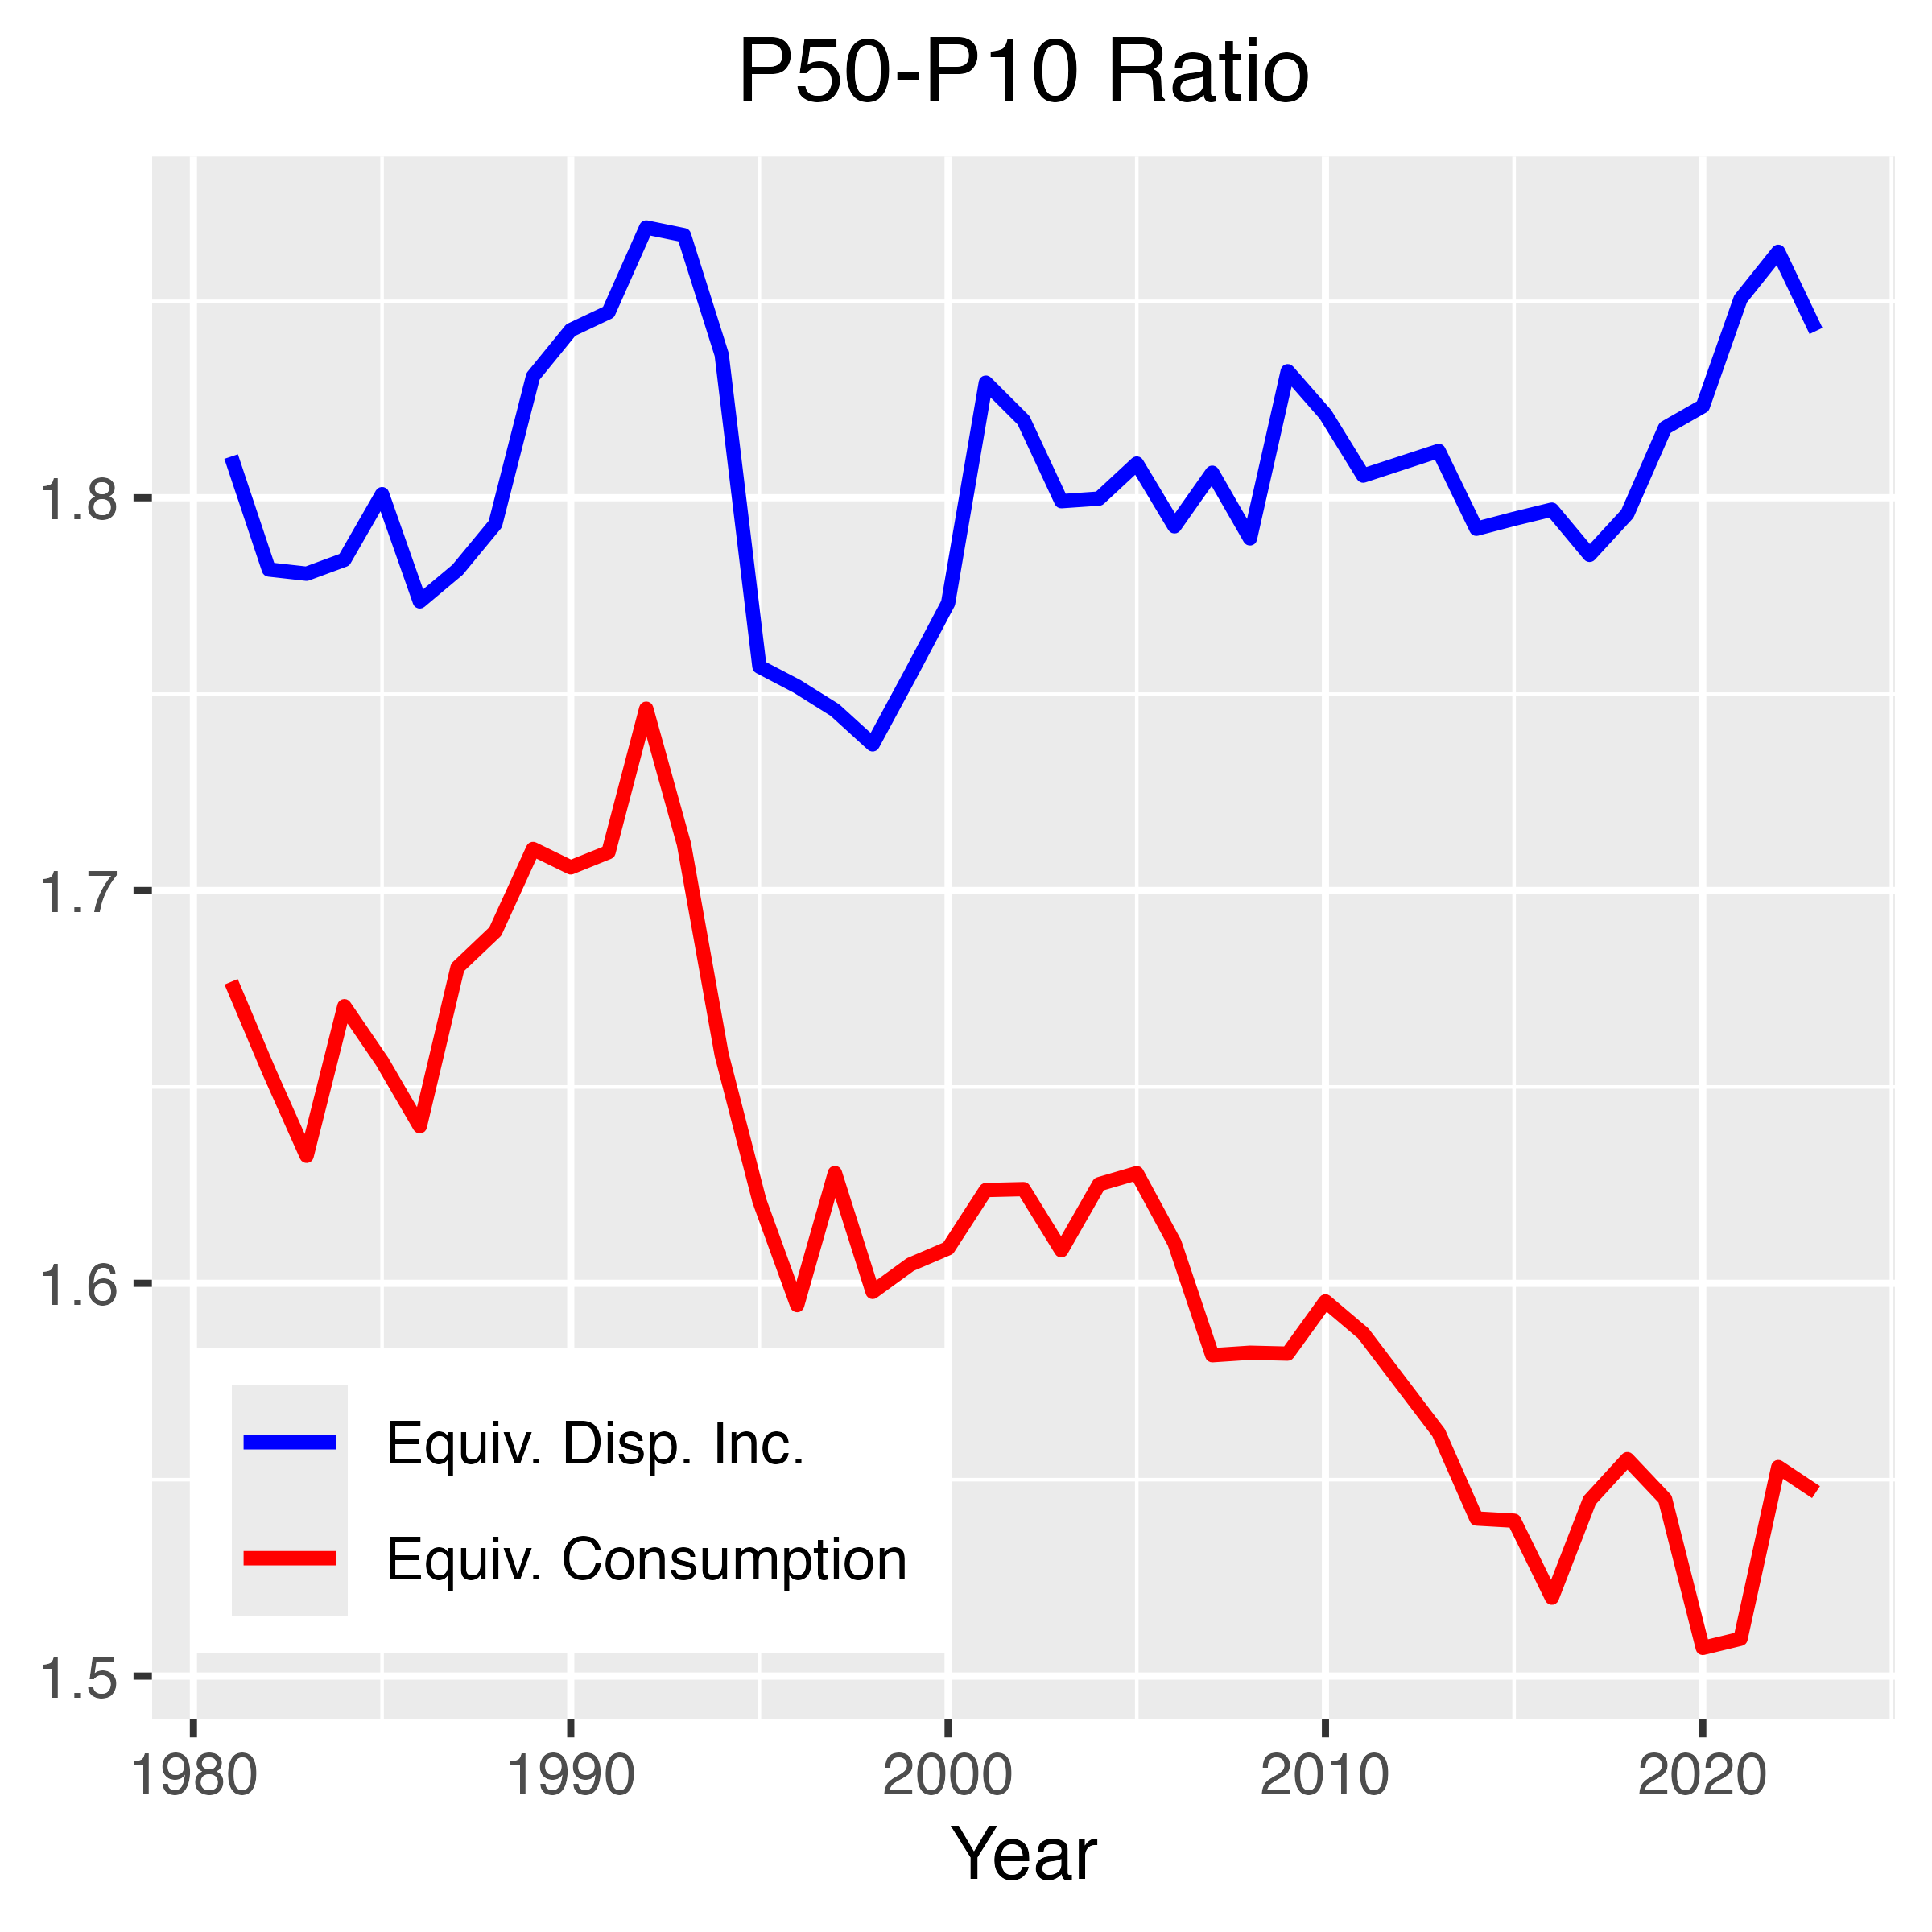
\includegraphics[width=\textwidth]{figures/Fig_6/Fig_6c.png}
        \label{fig:Consumption_P50_P10}
    \end{subfigure}
    \begin{subfigure}[t]{0.475\textwidth}
        \centering
        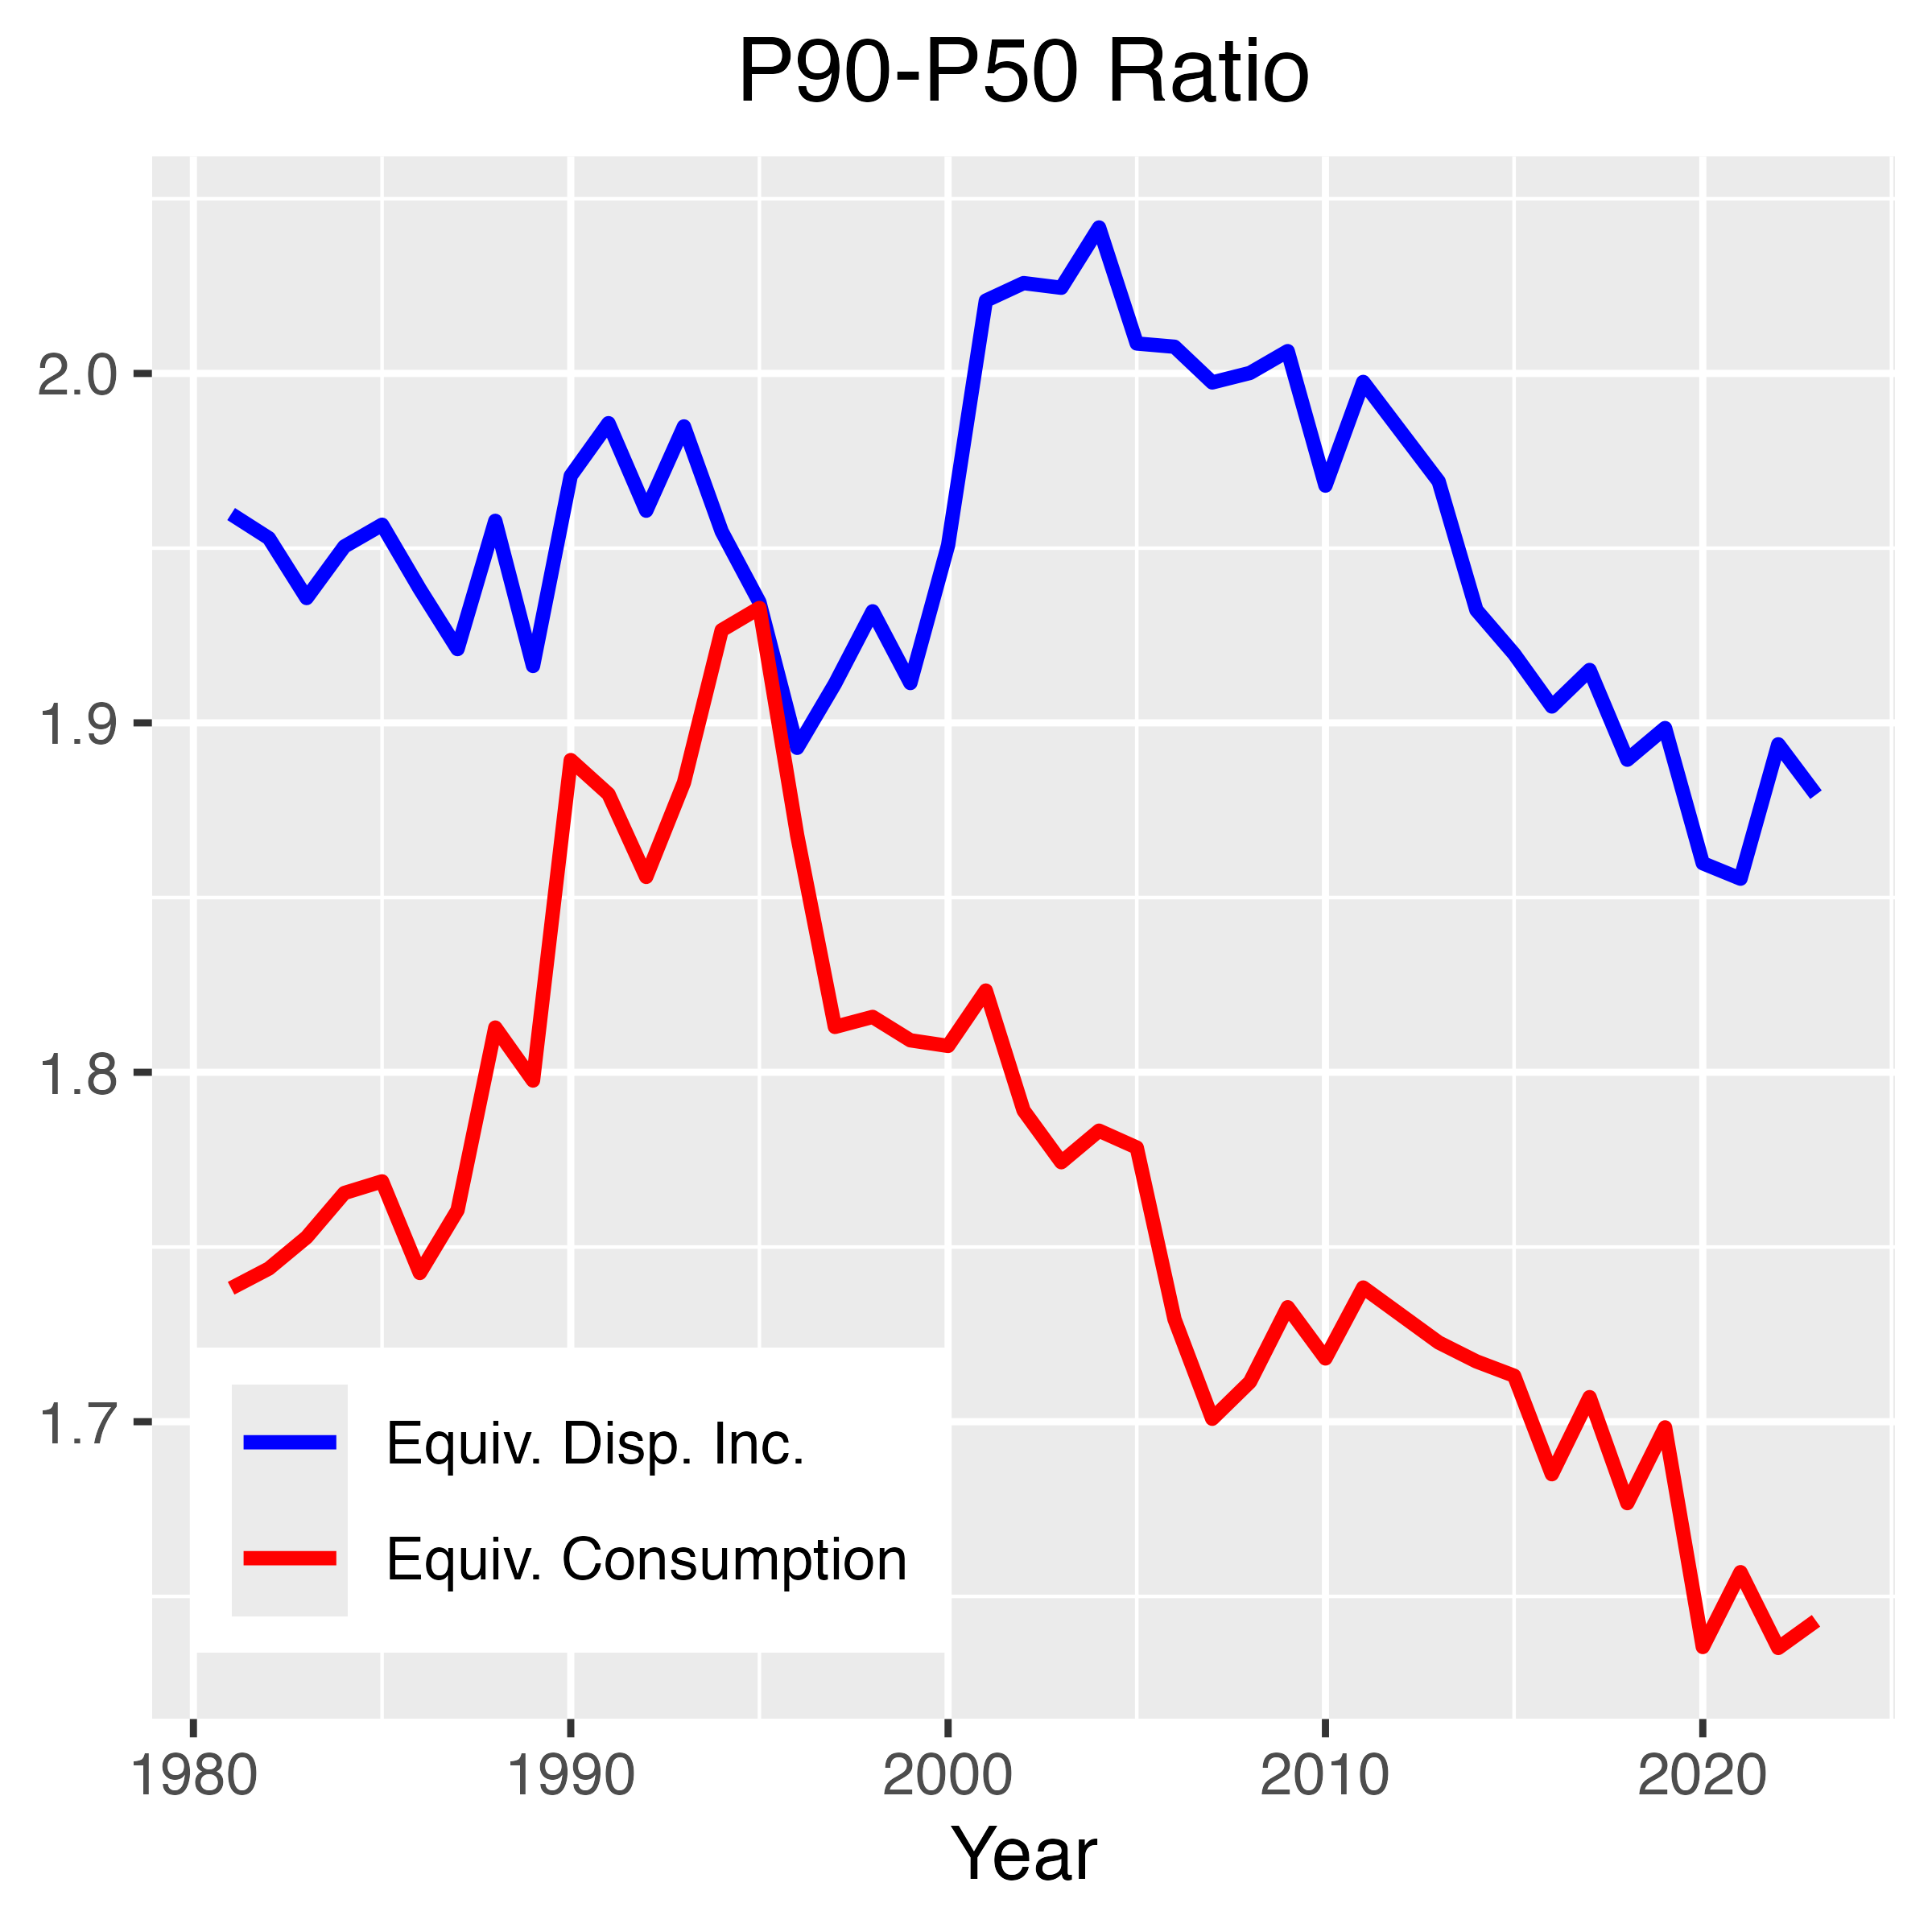
\includegraphics[width=\textwidth]{figures/Fig_6/Fig_6d.png}
        \label{fig:Consumption_P90_P50}
    \end{subfigure}
    \caption{From Disposable Income to Consumption}
    \label{fig:Consumption}
\end{figure}

\subsection{Cyclical Dynamics of Consumption Inequality}

\begin{figure}
    \centering
    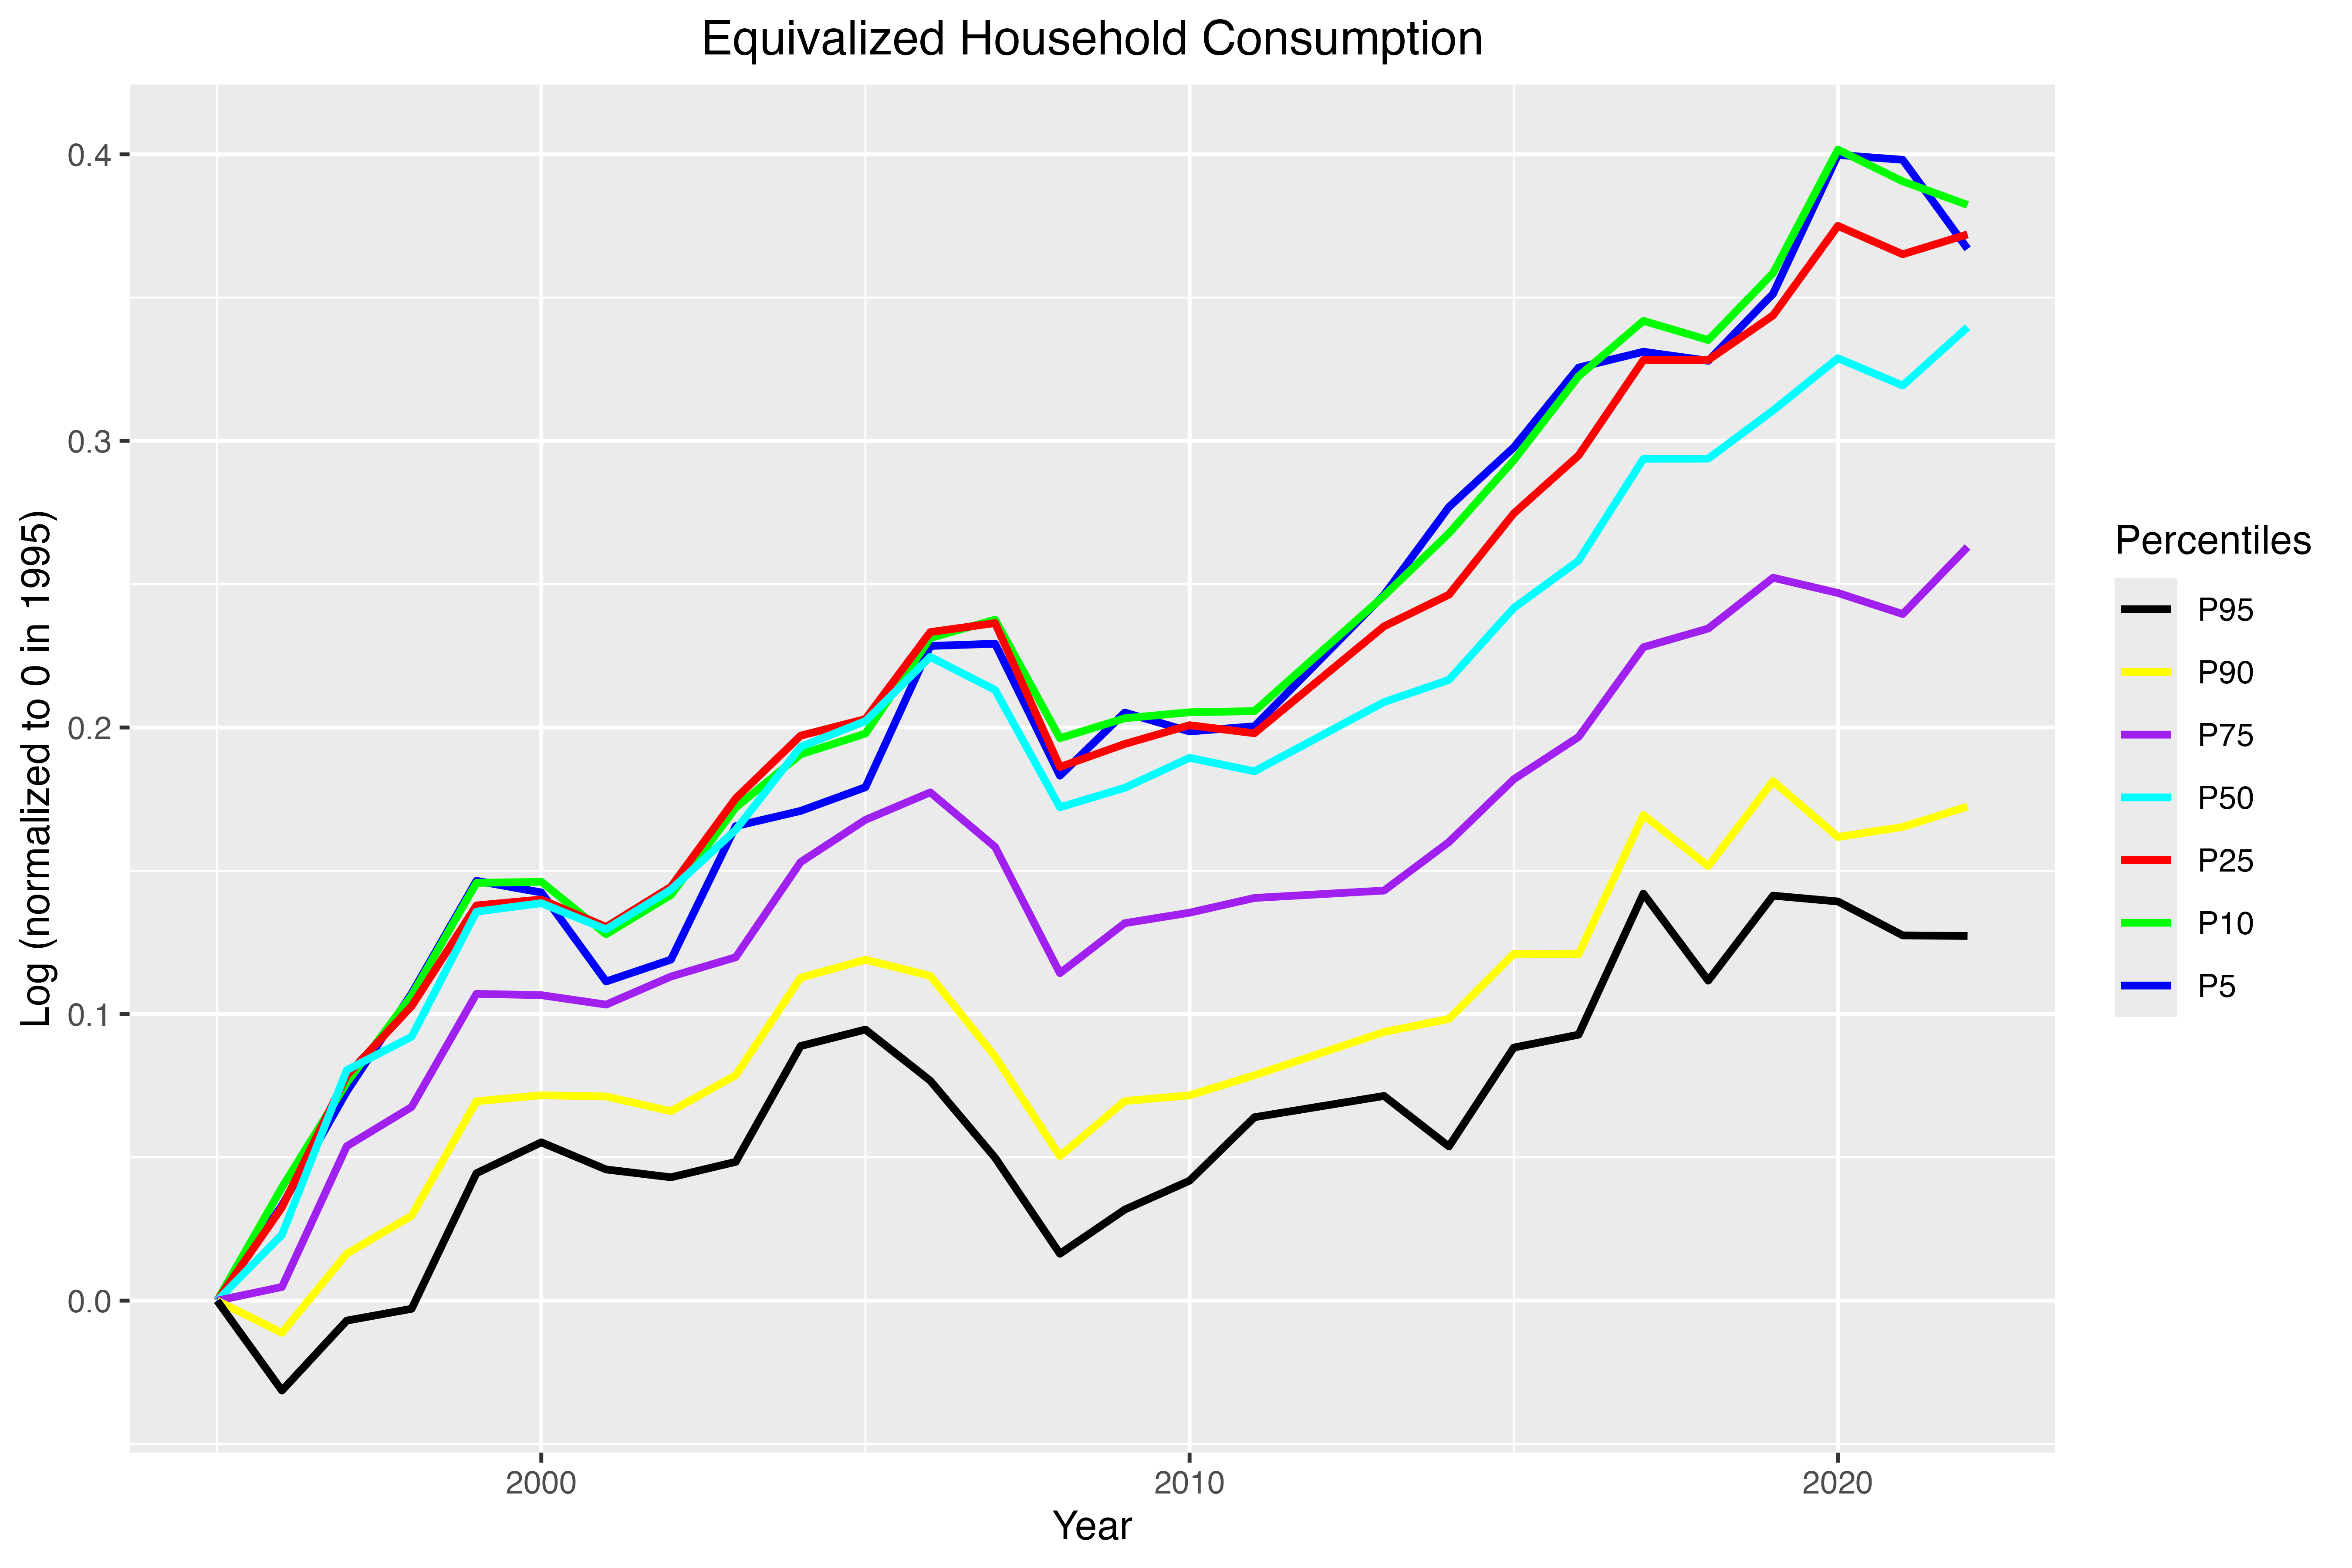
\includegraphics[width=0.95\textwidth]{figures/Fig_7/Fig_7_percentiles_a1995.png}
    \caption{Percentiles of the Household Consumption Distribution}
    \label{fig:Consumption_cyclic}
\end{figure}

\subsection{Food Consumption and Housing Services}

\begin{figure}
    \centering
    \begin{subfigure}[t]{0.475\textwidth}
        \centering
        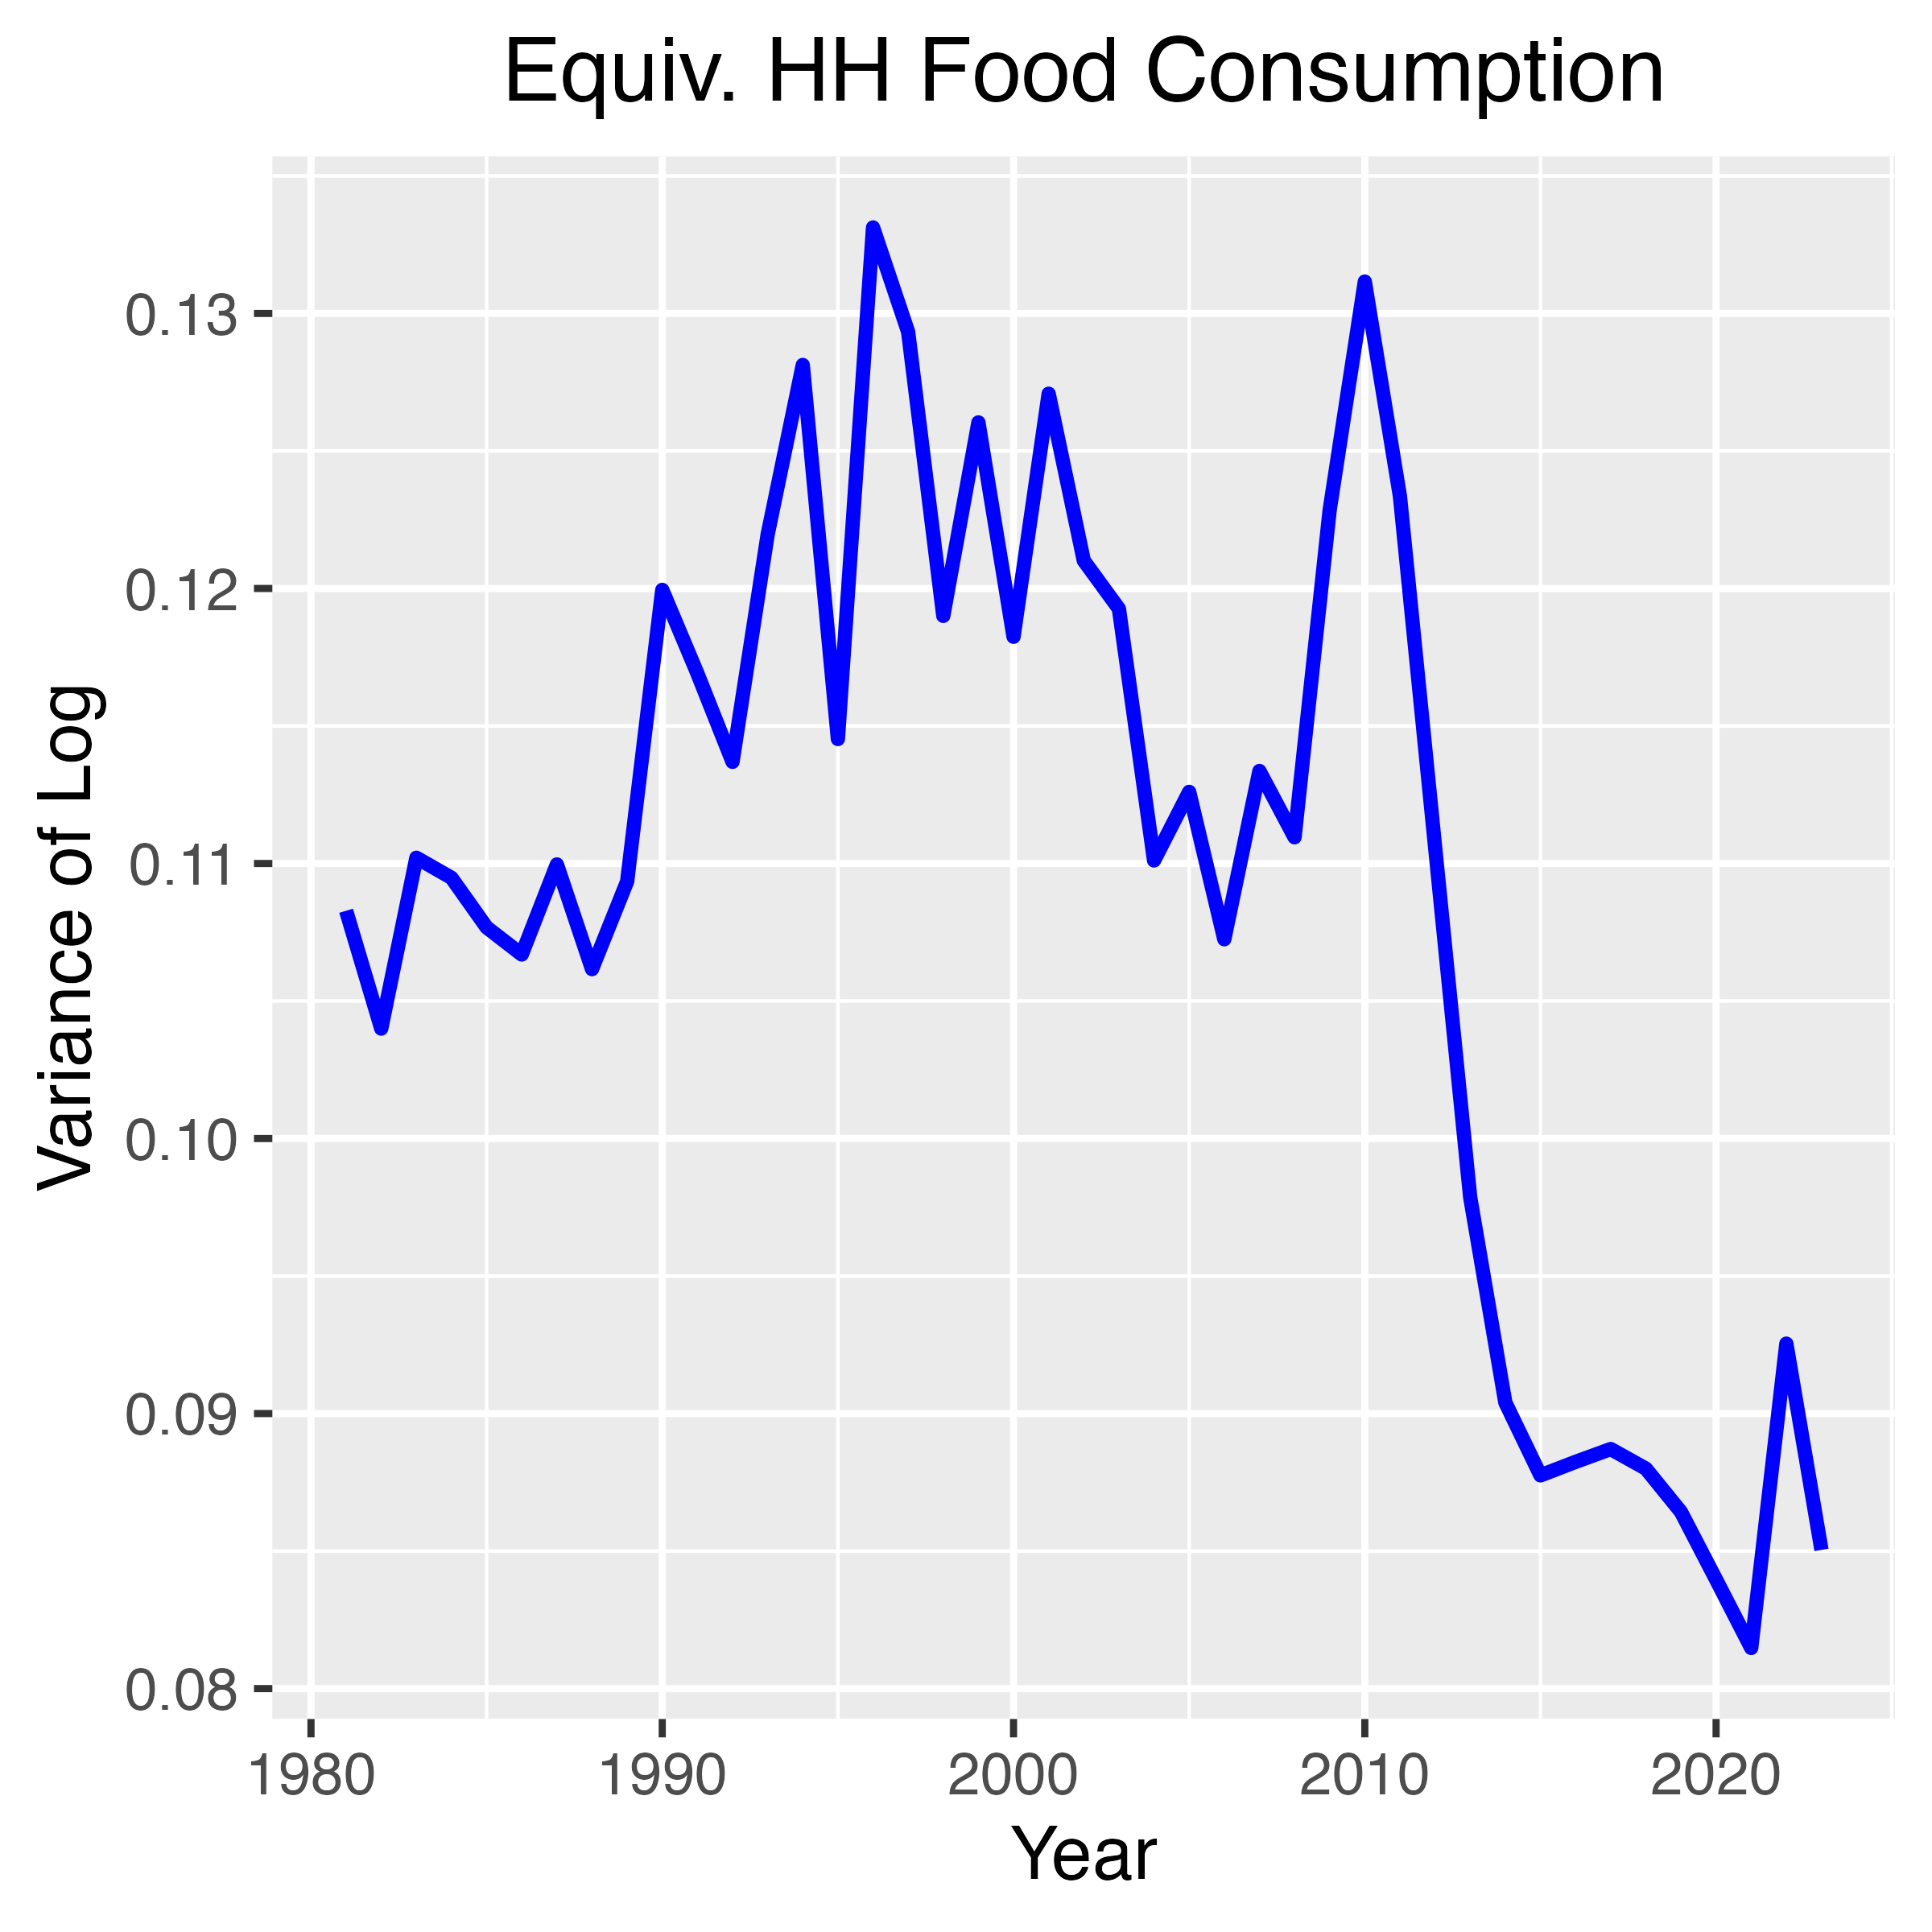
\includegraphics[width=\textwidth]{figures/Fig_8/Fig_8a_Var_Food.png}
        \label{fig:Food_Var}
    \end{subfigure}
    \begin{subfigure}[t]{0.475\textwidth}
        \centering
        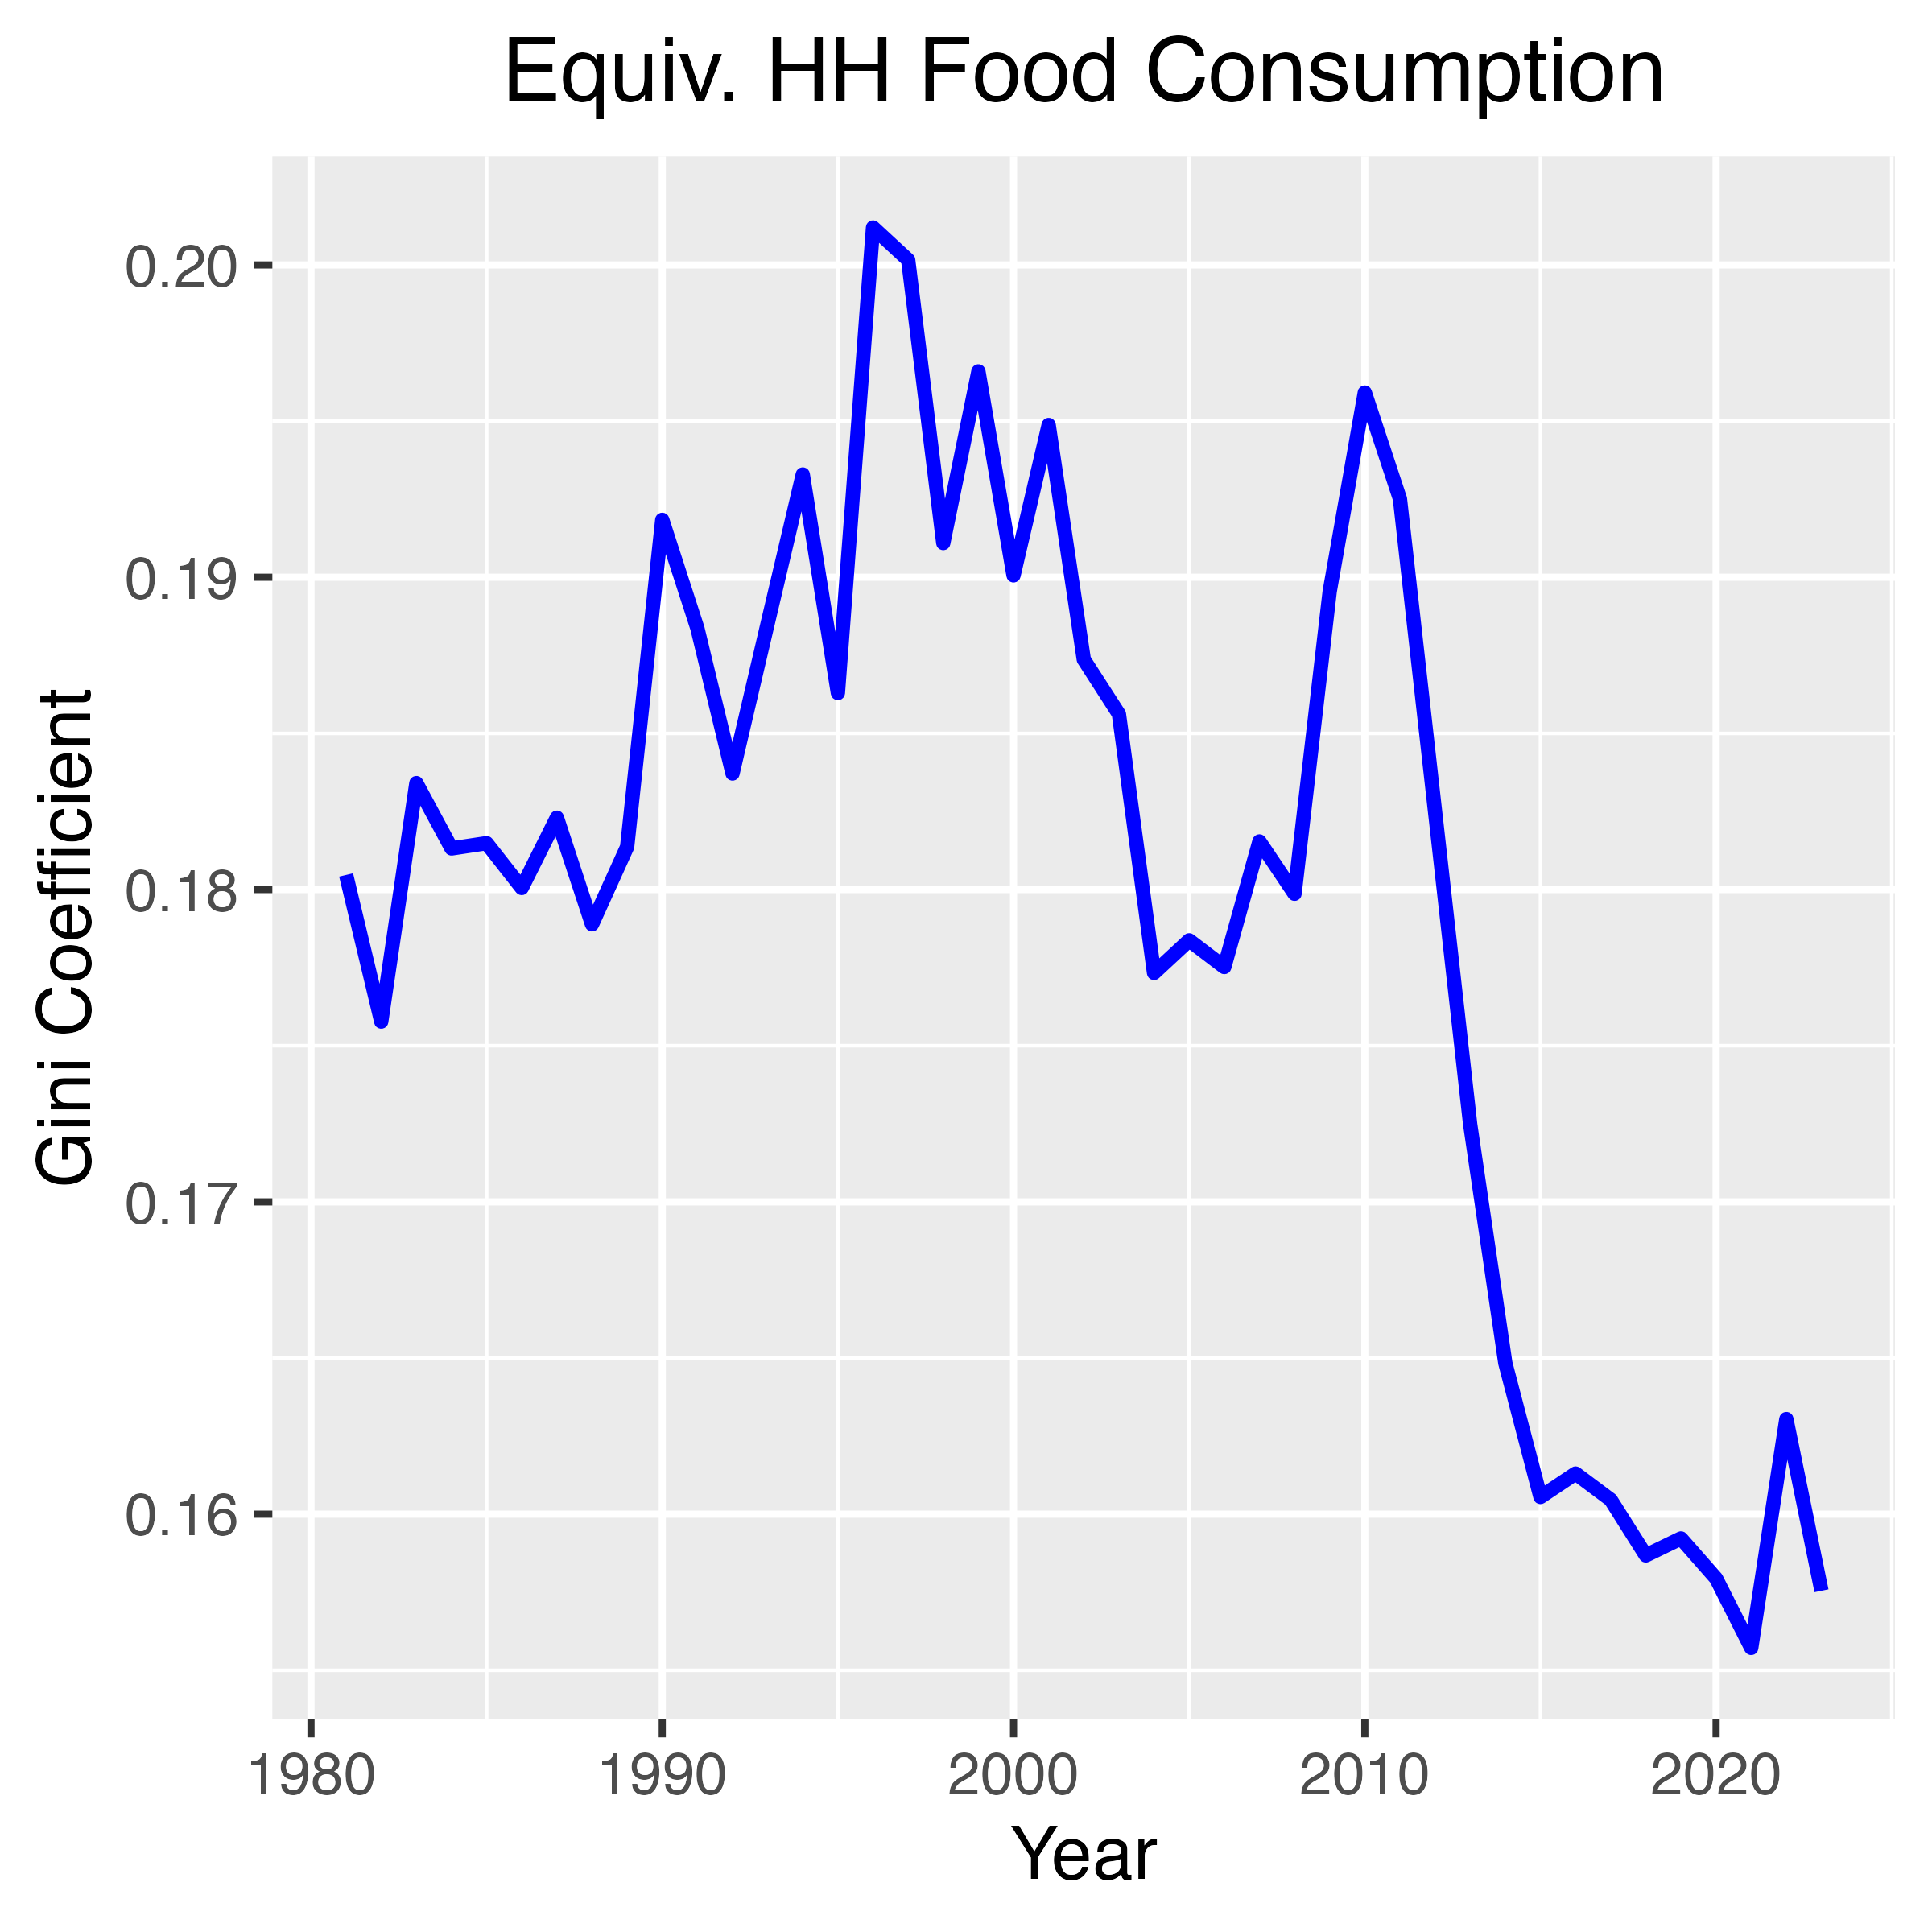
\includegraphics[width=\textwidth]{figures/Fig_8/Fig_8b_Gini_Food.png}
        \label{fig:Food_Gini}
    \end{subfigure}
    \begin{subfigure}[t]{0.475\textwidth}
        \centering
        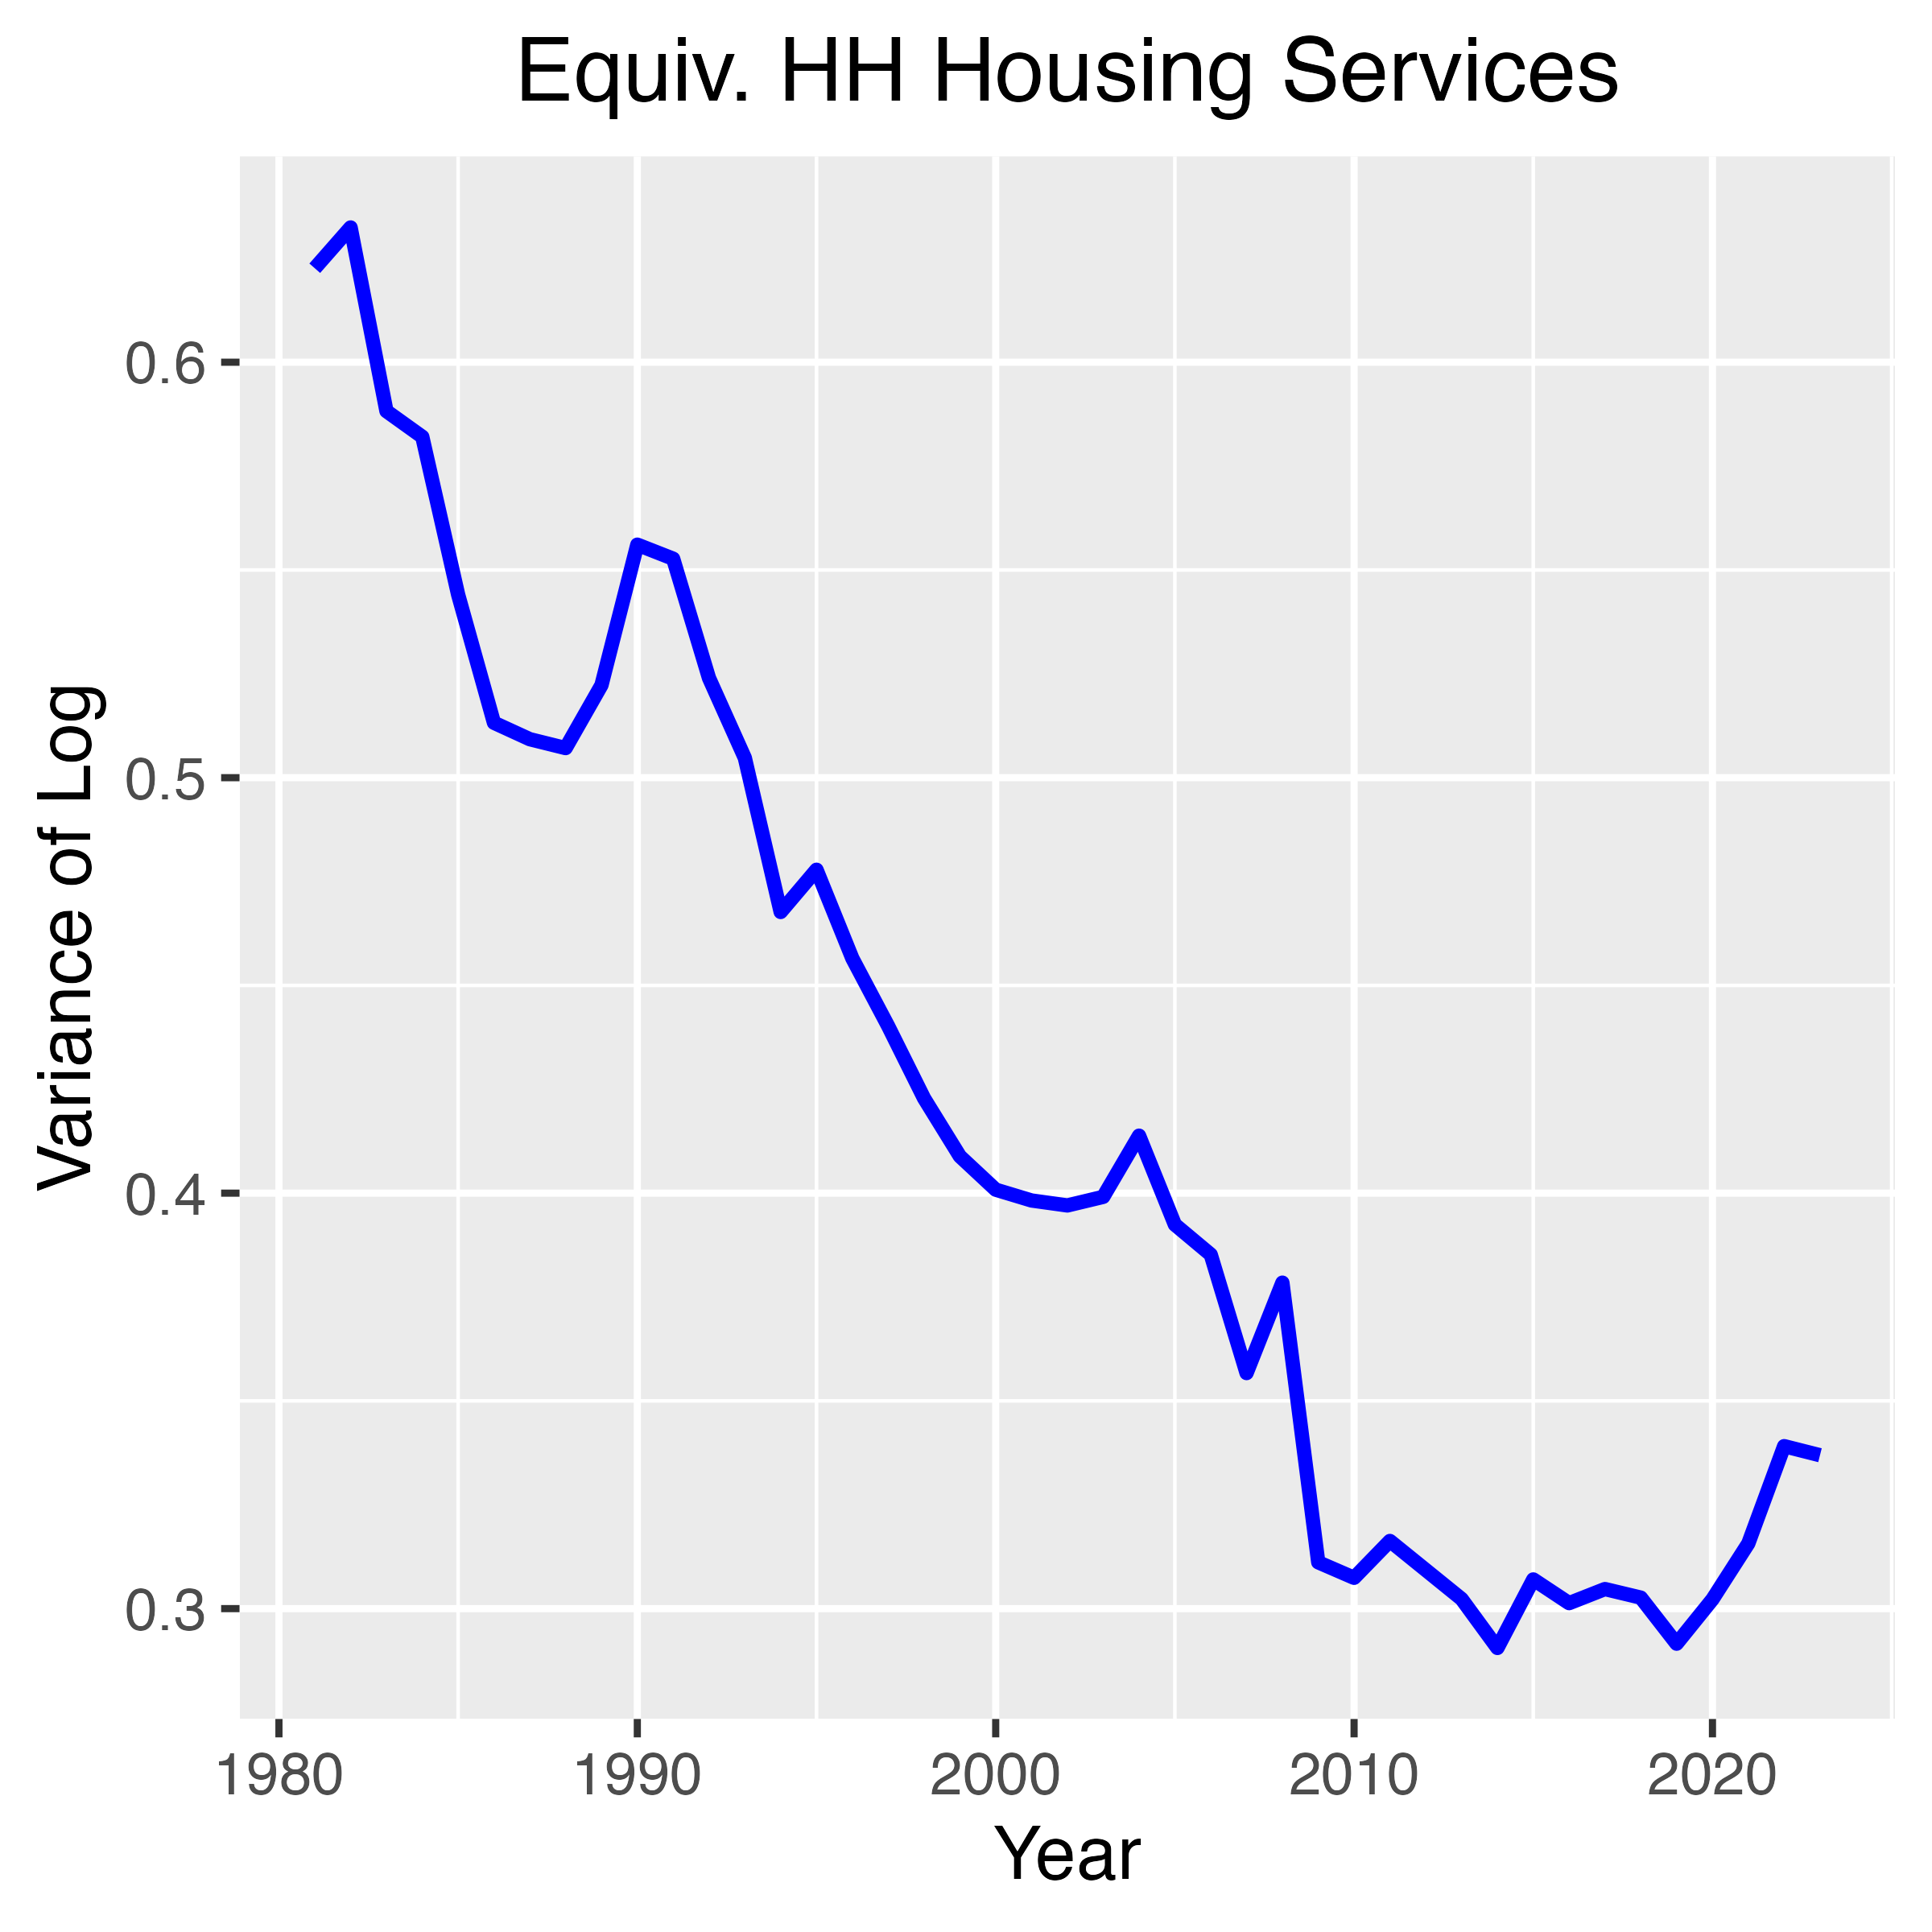
\includegraphics[width=\textwidth]{figures/Fig_8/Fig_8c_Var_Housing.png}
        \label{fig:Housing_Var}
    \end{subfigure}
    \begin{subfigure}[t]{0.475\textwidth}
        \centering
        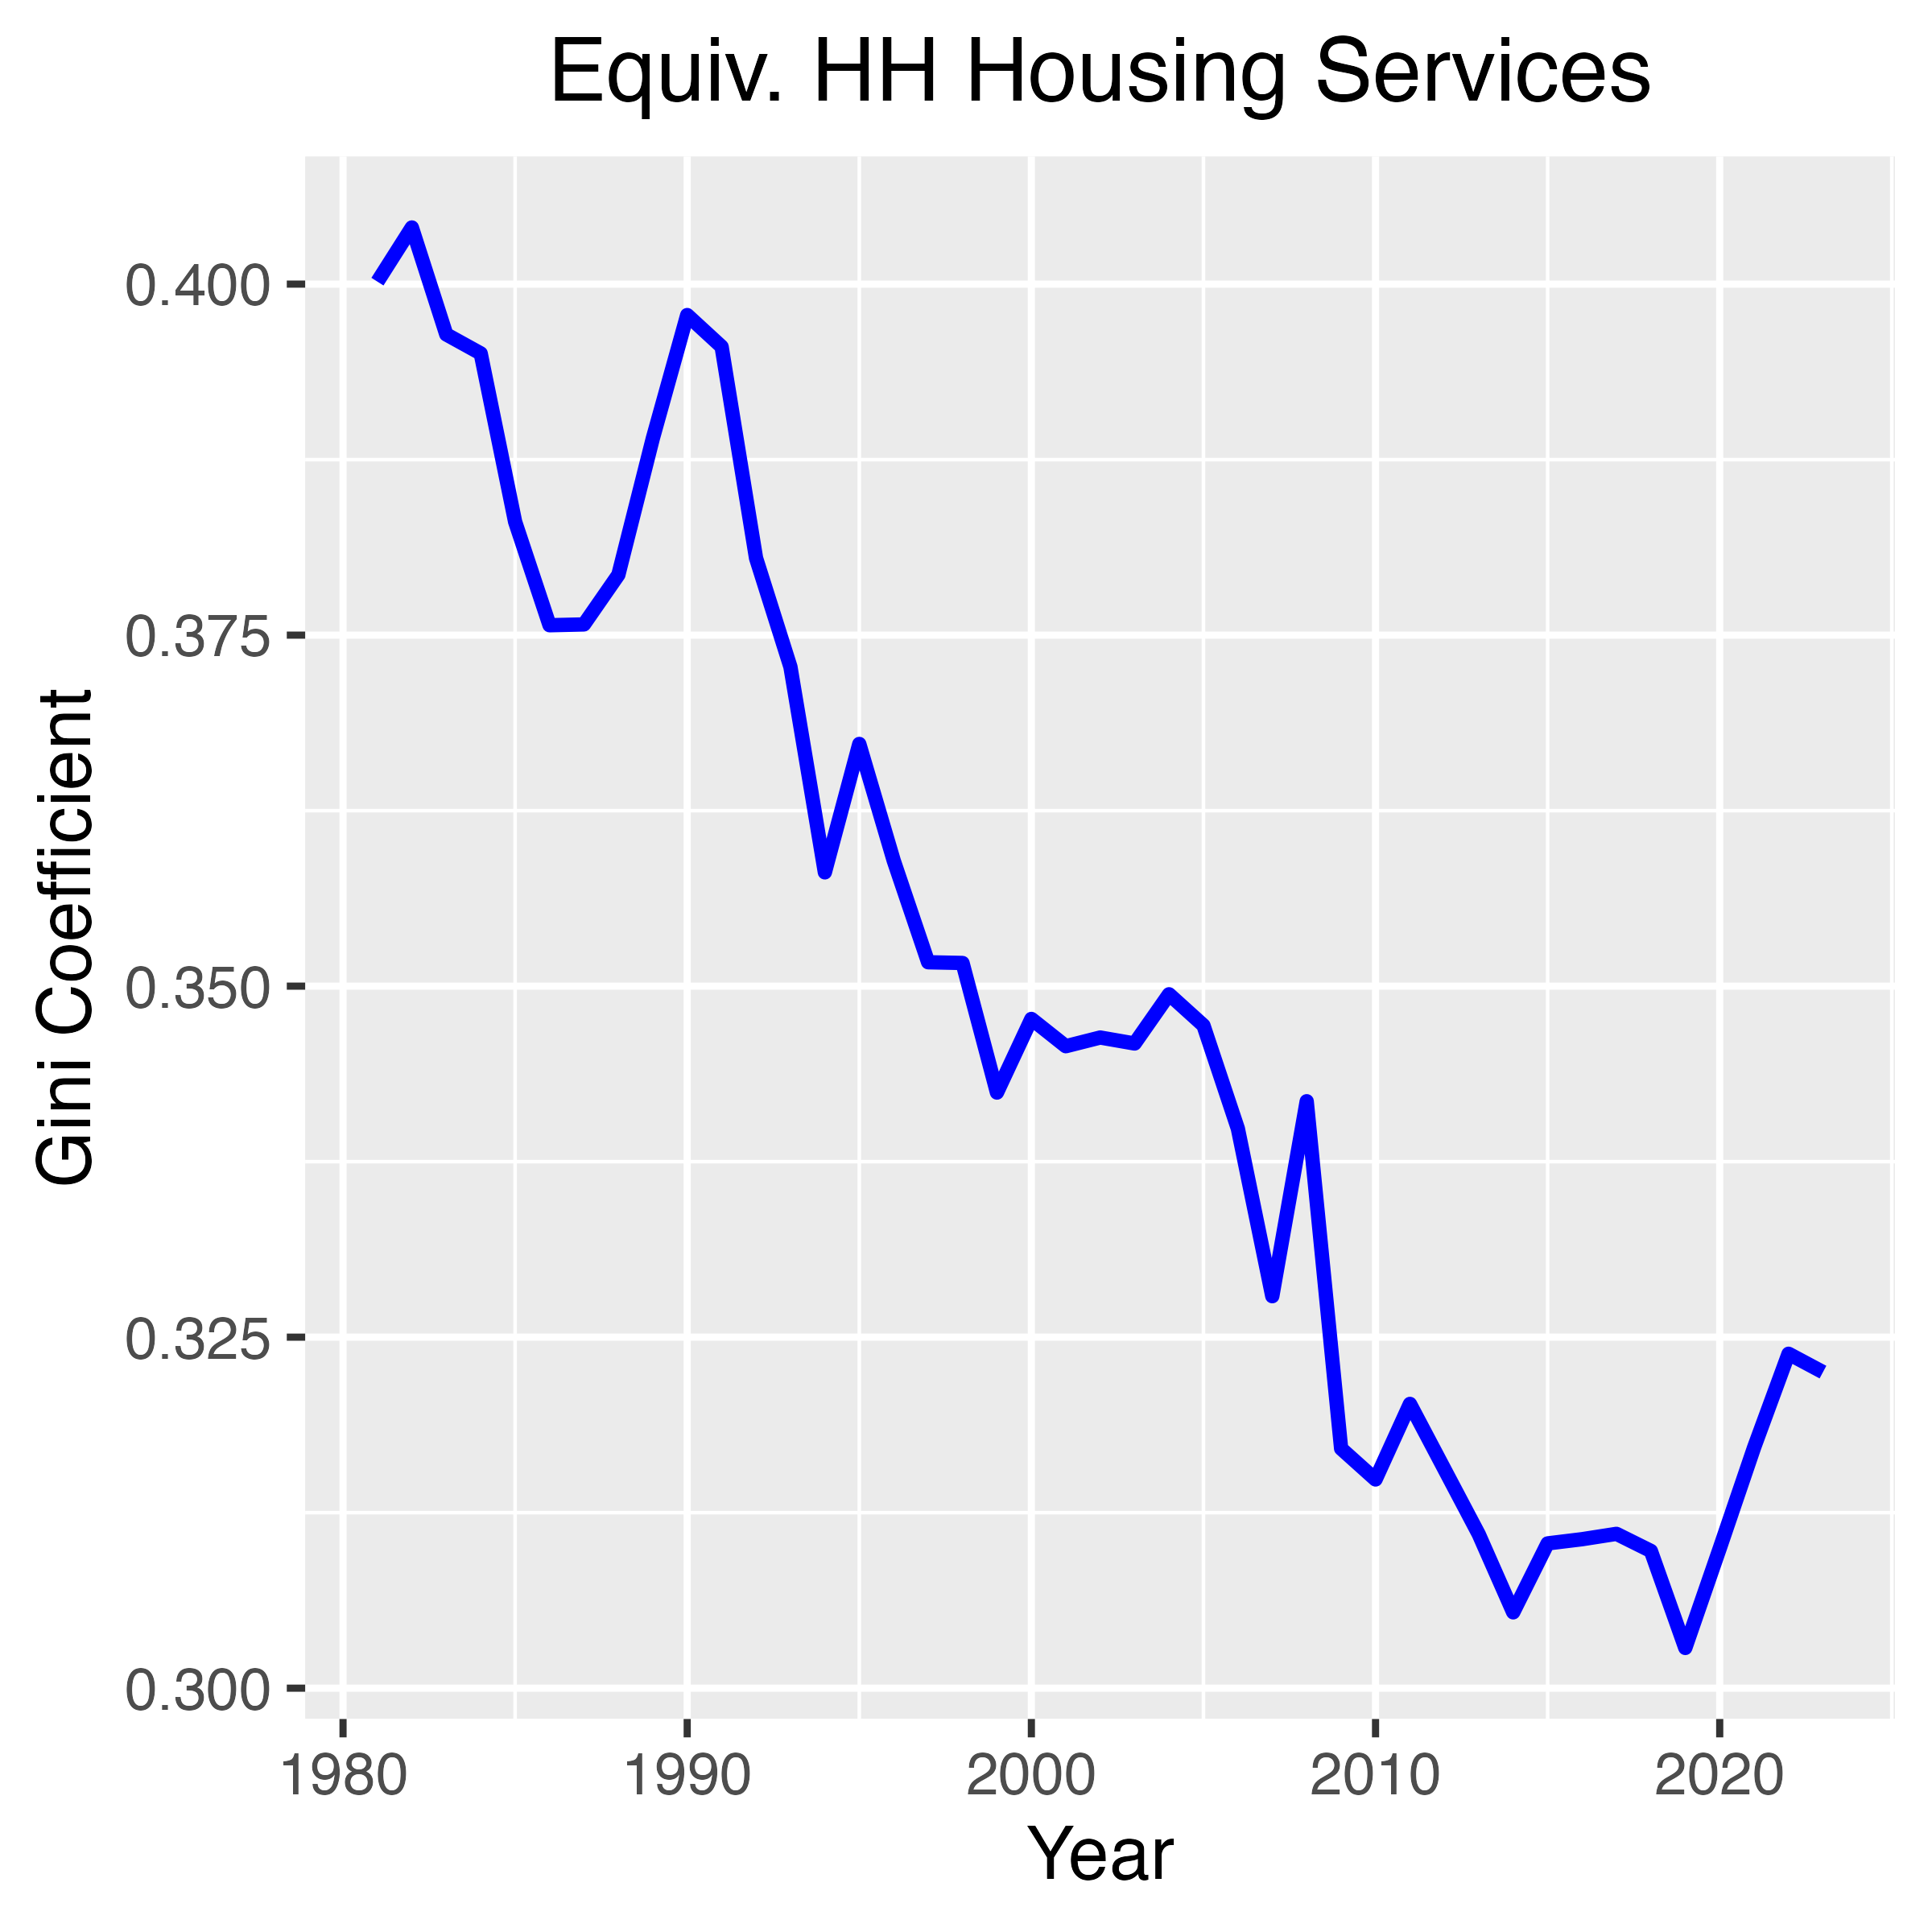
\includegraphics[width=\textwidth]{figures/Fig_8/Fig_8d_Gini_Housing.png}
        \label{fig:Housing_Gini}
    \end{subfigure}
    \caption{Food and Housing Consumption Inequality}
    \label{fig:Food_Housing}
\end{figure}


\section{Conclusion}
\label{sec:conclusion}


\end{document}